% \documentclass{cumcmthesis}
\documentclass[withoutpreface,bwprint]{cumcmthesis} %去掉封面与编号页,电子版提交的时候使用。


\usepackage[noend]{algpseudocode}
\usepackage{algorithm}
\usepackage{algpseudocode}
\usepackage{amsmath}
\usepackage[framemethod=TikZ]{mdframed}
\usepackage{url}   % 网页链接
\usepackage{subcaption} % 子标题
\usepackage{threeparttable} 
\title{面向不确定性与系统复杂性的农作物种植策略优化研究}
\tihao{A}
\baominghao{4321}
\schoolname{XX大学}
\membera{ }
\memberb{ }
\memberc{ }
\supervisor{ }%辅导老师
\yearinput{2023}
\monthinput{9}
\dayinput{8}

\setcounter{tocdepth}{2}

\begin{document}

\maketitle
\begin{abstract}
在乡村现代化与土地资源高效利用的背景下,本研究聚焦于农业生产中的资源配置优化问题。针对华北某山区乡村,旨在制定一个覆盖2024至2030年的最优农作物种植方案。该乡村的生产决策面临土地异质性、多重农艺规则以及田间管理便利性等一系列硬性约束,构成了一个复杂的约束优化环境。为应对此挑战,本文通过从\textbf{静态确定性规划、风险规避下的鲁棒优化到动态仿真优化}的递进式模型体系,旨在为该乡村提供兼顾经济效益最大化与风险稳健性的数据驱动型决策支持。

针对问题一,我们在所有经济与生产参数保持不变的确定性假设下,构建了一个\textbf{混合整数线性规划(MILP)模型}。该模型遵循\textbf{微观经济学}中\textbf{厂商利润最大化原则},在给定的生产技术与资源下,求解最优生产组合。我们分别探讨了当边际产出超出市场预期时,产品滞销或以折价销售的两种情景。鉴于该组合优化问题的计算复杂性,我们设计并实现了一种\textbf{修复式遗传算法}进行求解。结果表明,在滞销情景下,七年最优总利润为2987.65万元;在降价出售情景下,该值可提升至4191.35万元。

针对问题二,题目放宽了确定性假设,引入了市场与生产环境中的不确定性。模型将亩产量、预期销售量和销售价格等关键参数处理为在预设区间内波动的随机变量。为管理由此产生的风险,我们建立了一个\textbf{鲁棒优化模型},其目标从最大化期望利润转变为最大化风险规避下的年度平均保底利润。通过采用\textbf{多种群遗传算法(MPGA)}求解,并基于\textbf{风险调整后收益(夏普比率)}进行方案选择,最终确定了夏普比率最高(63.07)的种植方案。该方案在确保4310.00万元最低利润的同时,实现了4415.00万元的期望利润,获得了更优的风险-收益权衡。

针对问题三,我们在模型中进一步引入了\textbf{市场动态反馈机制},以反映供给变化对市场均衡价格与要素成本的影响。通过构建基于\textbf{价格与成本敏感度系数的仿真优化模型},我们分析了乡村作为市场参与者的行为对自身经济环境的反作用。模型继续使用\textbf{多种群遗传算法},在集成了\textbf{蒙特卡洛模拟}的适应度评估框架下进行求解。最终得到的自适应种植策略,其预期七年平均总利润为3902.05万元。利润分布的统计分析显示,方案收益高度稳定,有95\%的概率实现不低于3865.18万元的总利润。

为检验模型结果的稳健性,本文进一步执行了系统的灵敏度分析。分析识别出高价值作物的销售价格是影响确定性方案利润的关键因素。针对鲁棒模型,分析量化了不确定性范围与保底利润水平之间的关系,并通过后验模拟验证了鲁棒方案在降低收益波动方面的有效性。针对动态反馈模型,分析结果表明,将市场反馈机制纳入模型能够引导策略获得更高的期望收益,证实了模型设定的合理性。该系列分析增强了最终方案的可靠性,为其实际应用提供了支持。



\keywords{混合整数线性规划 \quad 鲁棒优化 \quad 仿真优化 \quad 修复式遗传算法 \quad 蒙特卡洛模拟 \quad 微观经济学 \quad 市场动态反馈机制}


\end{abstract}







\section{问题背景}

古代丝绸之路不仅是商贸通道,也是文化与技术交流的重要桥梁,其中,玻璃制品是早期东西方物质文化交流的重要物证。早期玻璃制品由西亚和埃及地区传入,其技术与风格影响了中国本土的玻璃制造业。中国古代工匠在吸收外来技术的基础上,利用本土原料进行生产,制造出外观相似但化学成分体系相异的玻璃器物。这种成分上的差异为鉴别古代玻璃制品的产地与技术来源提供了客观依据。

玻璃的主要成分为二氧化硅 ($SiO_2$)。为降低其熔点,制造过程中需加入助熔剂。古代中西方采用的助熔剂体系不同,形成了成分各异的玻璃类别。例如,以草木灰为助熔剂的钾玻璃 ($K_2O$ 含量较高) 和以铅矿石为助熔剂的铅钡玻璃 ($PbO$、$BaO$ 含量较高),后者被普遍认为是古代中国独立发展的玻璃品种。然而,玻璃制品在长期埋藏过程中,其表面易与环境发生元素交换,导致化学成分发生改变,这一风化过程给准确的成分分析与类型鉴别带来了挑战。因此,需要建立一套系统的数据分析方法,以消除或减弱风化作用的干扰,准确识别玻璃文物的化学成分规律,并对其进行科学分类与鉴别。


\begin{figure}[htbp]
    \centering
    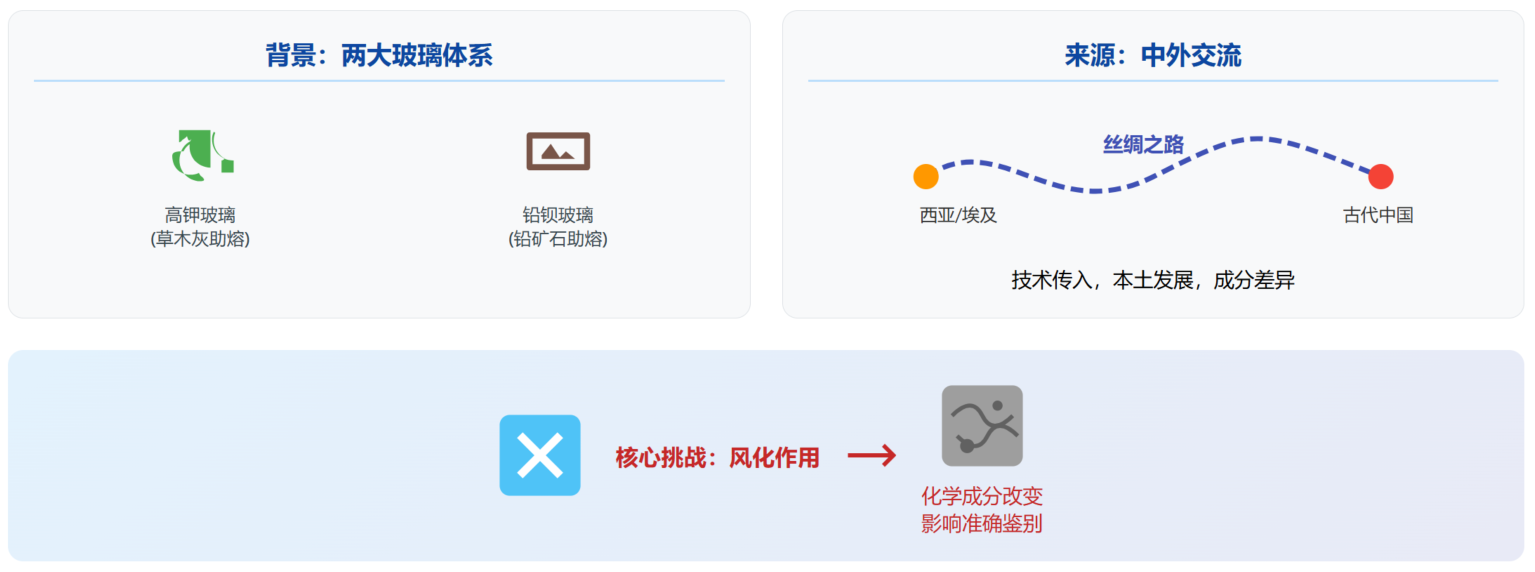
\includegraphics[width=\textwidth]{figs/1前置/问题背景.png}
    \caption{问题背景} 
    \label{fig:your_image_label} 
\end{figure}


\section{问题重述}

问题一:分析玻璃文物表面风化状态与其玻璃类型、纹饰和颜色等物理属性的统计关系。在此基础上,结合玻璃类型,研究表面风化对化学成分含量的影响规律,并建立数学模型,根据风化样品的化学成分数据,预测其风化前的成分含量。

问题二:根据已分类的高钾玻璃与铅钡玻璃的化学成分数据,建立有效的分类判据。进而,在每个大类中,选择合适的化学成分作为指标,对该类别进行亚类划分,并给出具体的划分方案。最后,对分类与划分结果的合理性及稳定性进行分析。

问题三:利用已建立的分类模型,对一批未知类别的玻璃文物样品的化学成分数据进行分析,鉴别其所属的玻璃类型。同时,需要对鉴别结果的敏感性进行评估,以考察分类结果的稳健程度。

问题四:针对高钾玻璃与铅钡玻璃两个类别,分别探究其内部各化学成分之间的关联关系。通过比较两个类别在化学成分关联模式上的异同,表现不同玻璃体系在原料构成与制造工艺上可能存在的差异。

\section{问题分析}

对于问题一,该问题包含两个递进的部分。第一部分要求分析风化状态与玻璃类型、纹饰、颜色等多个定性变量之间的关系,可采用列联表分析与卡方检验等统计方法,检验这些变量之间是否存在显著的相依性。第二部分旨在建立风化前后化学成分的映射关系。此过程可视为一个回归或预测问题,可以通过分析同一文物上风化点与未风化点的成分差异,建立多元回归模型,从而实现对风化前成分的定量估计。

对于问题二,其核心是分类与聚类任务。首先,区分高钾与铅钡玻璃是一个监督学习分类问题。由于类别标签已知,可利用逻辑回归、支持向量机或决策树等分类算法,建立基于化学成分的分类器。其次,在已确定的类别内部进行亚类划分,是一个无监督学习的聚类问题。因缺乏亚类的先验标签,可采用K-均值聚类或层次聚类等算法,依据关键化学成分的分布特征进行探索性划分。对结果的合理性分析可通过交叉验证评估分类器性能,通过轮廓系数等指标评价聚类效果;敏感性分析则可通过扰动数据来检验模型输出的稳定性。

对于问题三,该问题是问题二所建分类模型的直接应用。需要将表单三中未分类样本的化学成分数据输入已训练好的分类器,以获得其预测类别。其敏感性分析旨在评估分类决策的可靠性,可以通过计算样本点到分类边界的距离或在样本成分数据上施加微小扰动,观察分类结果是否发生改变,来衡量分类的稳健性。

对于问题四,该问题要求探究不同类别玻璃内部化学成分的相互关系。此分析可通过计算各类别样本的协方差矩阵或相关系数矩阵来实现。皮尔逊相关系数是衡量两个连续变量间线性关系强度的常用指标。通过为高钾和铅钡玻璃分别构建相关系数矩阵,并利用热力图等可视化手段,可以直观地展示不同类别玻璃内部各元素间的协同或拮抗关系,比较其模式差异,为探究其工艺与原料来源提供数据支持。

% \section{数据预处理与分析}

为构建有效的种植策略优化模型,首先需要对研究背景中涉及的基础数据进行系统性的分析与处理。本章将围绕耕地资源特性、农作物种植条件及经济效益指标三个核心维度展开,旨在明确模型构建所需的基本参数与约束条件。


\subsubsection{数据预处理}



由于部分数据在数据表中带有空格后缀,影响数据读取,因此需对于单元格格式进行修改,将空格全部替换删除后,进行后续数据分析及模型建立。

根据附件2给出的信息,2023年智慧大棚第一季的数据均与普通大棚第一季的相同,利用给出的普通大棚第一季的数据将2023年智慧大棚第一季数据补全。

处理后的数据进行可视化后如\ref{fig:fig:2023年智慧大棚第一季数据}所示,可见处理后无缺失值。

\begin{figure}[htbp]
    \centering
    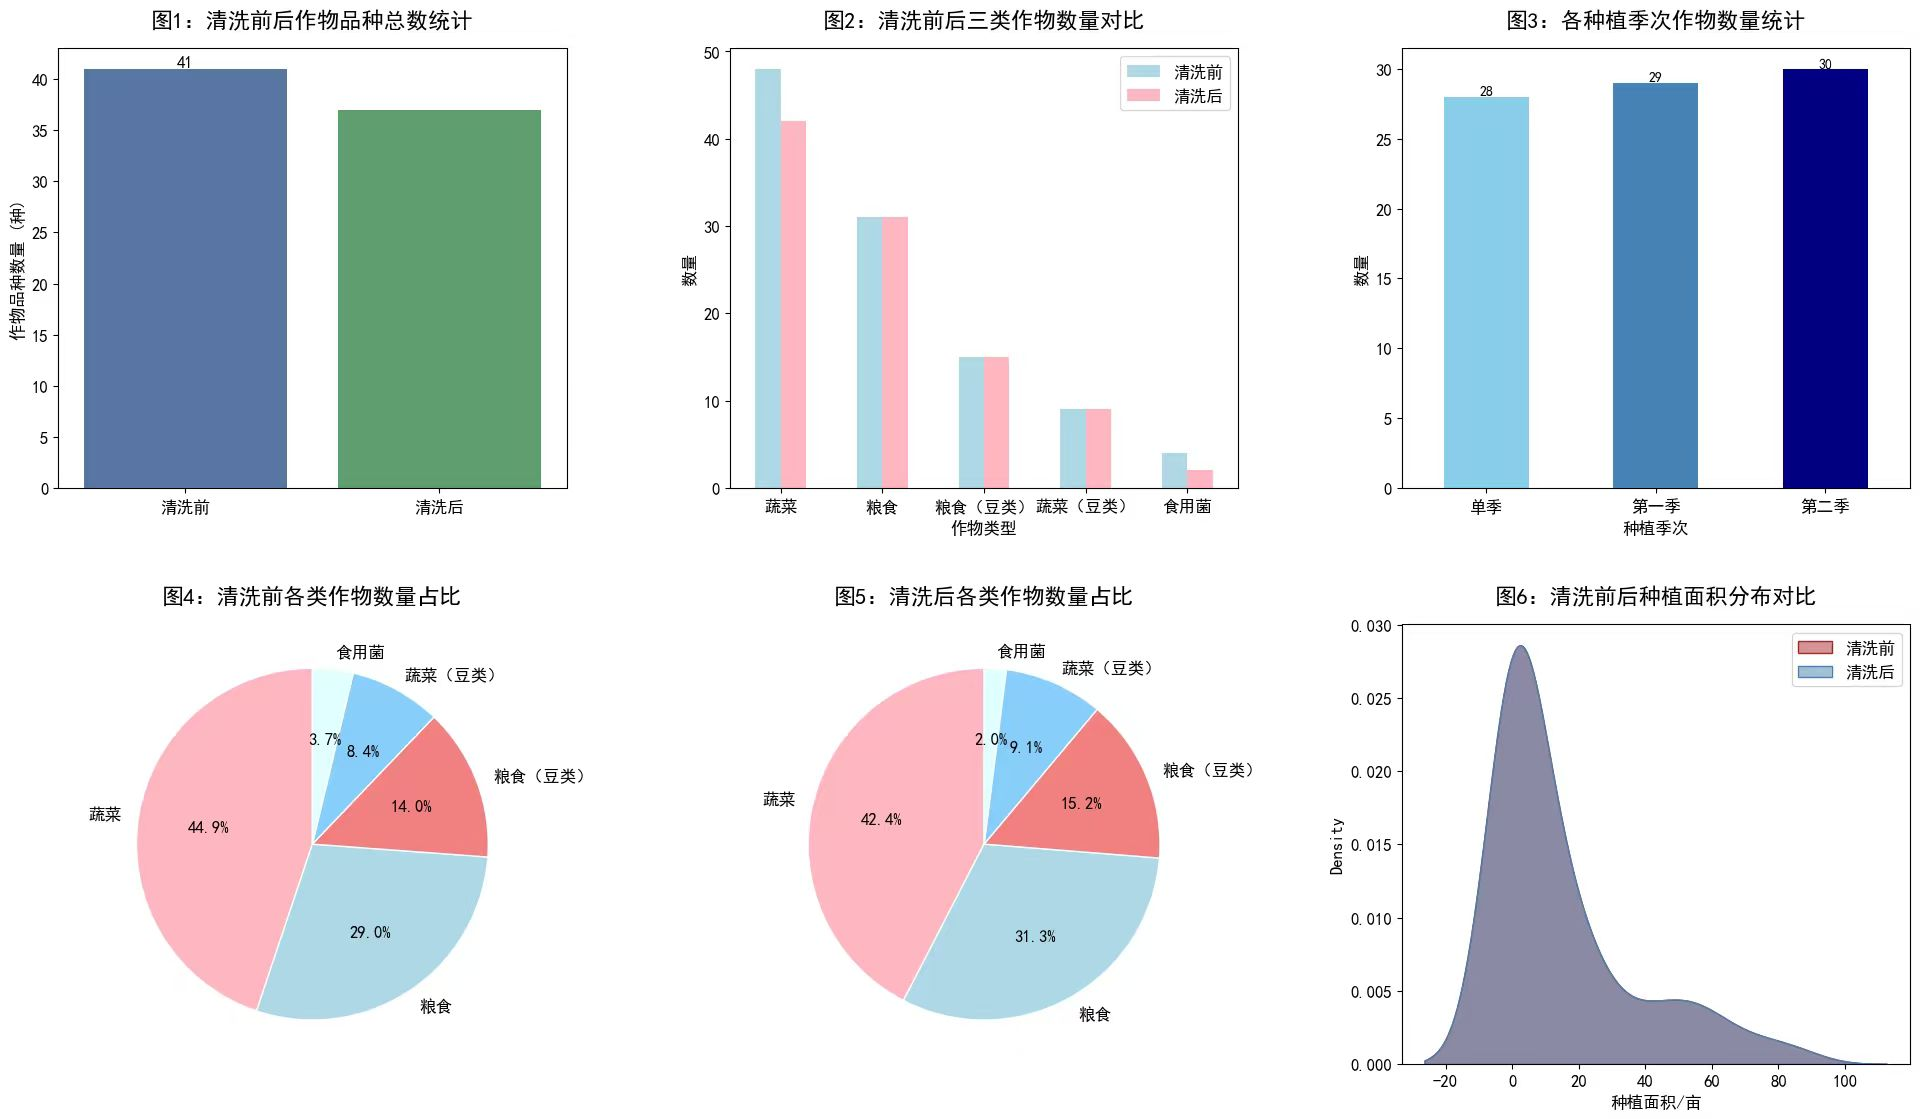
\includegraphics[width=0.8\textwidth]{figs/2数据分析与预处理/数据预处理后.jpg}
    \caption{完整数据可视化}
    \label{fig:2023年智慧大棚第一季数据}
\end{figure}

\subsection{耕地资源分析}

该乡村的耕地资源主要由露天耕地与大棚构成。根据附件数据,我们汇总了各类土地的面积与分布情况。图\ref{fig:land_distribution}直观地展示了不同类型土地资源的面积占比。

\begin{figure}[htbp]
    \centering
    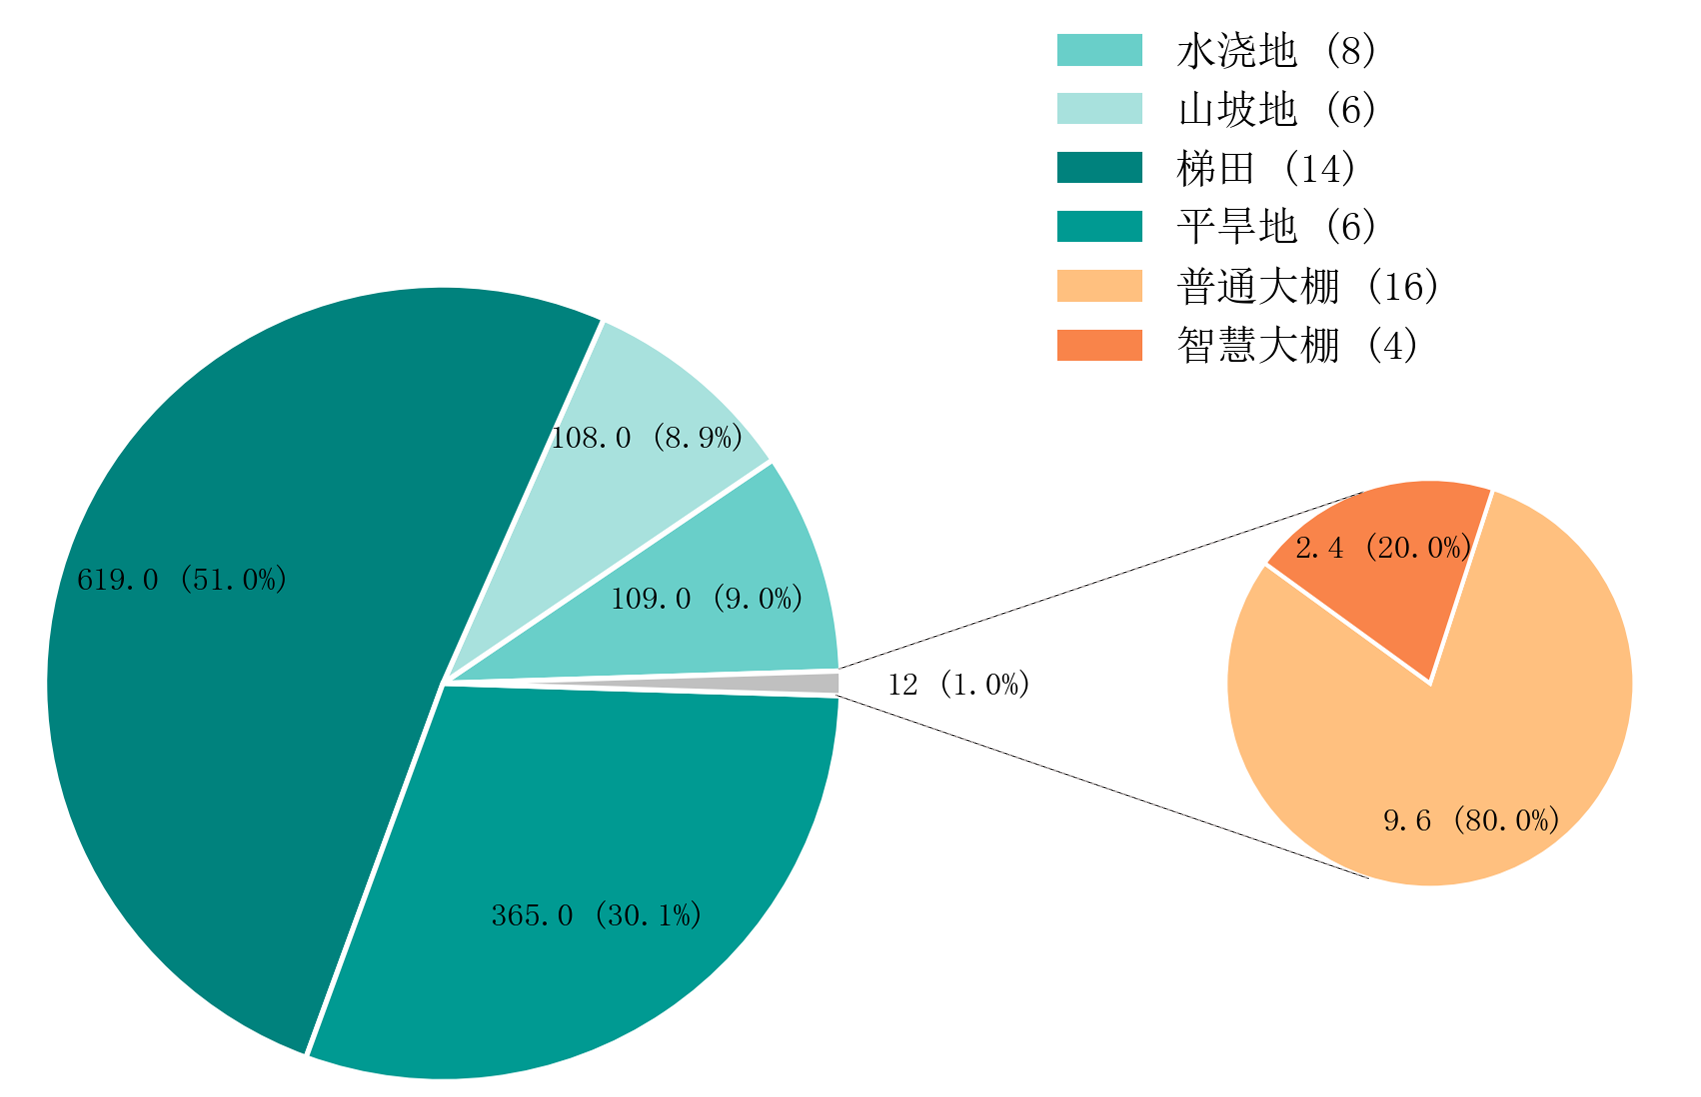
\includegraphics[width=0.8\textwidth]{figs/2数据分析与预处理/土地类型分布.png}
    \caption{土地类型分布情况}
    \label{fig:land_distribution}
\end{figure}

根据资料,不同类型的土地其物理特性与配套设施存在差异,从而决定了其适宜种植的作物类型与种植模式。
\begin{itemize}
    \item \textbf{平旱地(A)、梯田(B)与山坡地(C)}:这三类土地缺乏灌溉条件,农业生产完全依赖自然降水。此类土地环境适合种植耐旱、需水较少的单季粮食作物,不适宜水稻的生长。
    \item \textbf{水浇地(D)}:该类土地具备完善的灌溉设施,能够保障作物生长所需的水分。由于水稻的生长周期较长,若种植水稻则为单季种植。此外,该地块也可用于两季蔬菜的种植。从水资源供给角度看,第一季水源充足,适宜种植需水量较高的蔬菜;第二季为满足耐寒和简化管理的需求,种植作物限定为大白菜、白萝卜或红萝卜中的一类。
    \item \textbf{普通大棚(E)}:作为一种利用塑料薄膜或玻璃覆盖形成的设施农业,大棚内部形成了可控的小气候环境。其维护成本较高,因此不适宜种植附加值较低的粮食作物。棚内空间相对密闭,高温高湿的环境使得部分作物易受病虫害影响。同时,其土层较浅,不适合根系发达的蔬菜作物。因此,普通大棚适宜进行两季作物轮作,第一季可种植多种蔬菜,而第二季则种植对湿度和温度要求较低的食用菌。
    \item \textbf{智慧大棚(F)}:作为普通大棚的升级版本,智慧大棚通过现代技术手段实现对棚内温度、湿度、光照等环境因子的实时监控与调控。优化的生长环境使其能够支持两季蔬菜的种植,从而提高土地利用效率与产出。
\end{itemize}

\subsection{农作物种植条件分析}

基于对土地特性的分析,我们进一步梳理了各类农作物的具体种植要求。不同作物在作物类别、适种耕地、耕种时序等方面存在明确的划分,这些构成了种植决策的基本约束。表\ref{tab:crop_requirements}系统地总结了所有可选作物的种植要求。

\begin{table}[htbp]
    \centering
    % 使用 threeparttable 环境来管理标题、表格主体和脚注
    \begin{threeparttable}
        \caption{优化后的农作物种植要求}
        \label{tab:crop_requirements_optimized_1}
        % 使用 tabularx 环境,并设置总宽度为列宽 \columnwidth
        % X 列是一种特殊的列,可以自动伸展以填充可用空间
        \begin{tabularx}{\columnwidth}{l l >{\raggedright\arraybackslash}X l}
            \toprule
            作物类别 & 作物子类/名称 & 种植耕地 & 耕种时期 \\
            \midrule
            % 使用 \multirow 合并“粮食”类别下的三行
            \multirow{3}{*}{粮食}
            & 豆类 (黄豆、黑豆、豌豆等) & A, B, C & 单季种植 \\
            \addlinespace % 在行之间增加一点垂直空间,使分组更清晰
            & 谷物及薯类 (小麦、玉米、南瓜、红薯等) & A, B, C & 单季种植 \\
            \addlinespace
            & 水稻 & D & 单季种植 \\
            \midrule
            % 使用 \multirow 合并“蔬菜”类别下的三行
            \multirow{3}{*}{蔬菜}
            & 豆类 (豇豆、刀豆、芸豆) & D, E, F & 第一、二季 \\
            \addlinespace
            & 常见蔬菜 (番茄、黄瓜、菠菜等) & D, E, F & 第一、二季 \\
            \addlinespace
            & 大白菜、萝卜 & D & 第二季 \\
            \midrule
            食用菌 & 榆黄菇、香菇、羊肚菌等 & E & 第二季 \\
            \bottomrule
        \end{tabularx}
        % 使用 tablenotes 环境添加表格的脚注
        \begin{tablenotes}[flushleft]
            \footnotesize % 设置脚注字体为小号
            \item[备注] A=平旱地, B=梯田, C=山坡地, D=水浇地, E=普通大棚, F=智慧大棚。
        \end{tablenotes}
    \end{threeparttable}
\end{table}


从表\ref{tab:crop_requirements}可知,作物的种植选择与土地类型和种植季节严格对应。例如,粮食作物主要在A、B、C类土地上单季种植,而蔬菜和食用菌则主要分布在D、E、F类土地上,并存在明确的季节划分。

\subsection{经济效益指标分析}

为了对不同种植方案的优劣进行量化评估,需要分析各农作物的经济效益。我们基于2023年的相关统计数据,对该年度的作物总产量分布和单位亩利润进行了可视化分析。

图\ref{fig:production_distribution_2023}展示了2023年各种农作物的总产量情况。从中可以看出不同作物在乡村农业生产中所占的比重。

\begin{figure}[htbp]
    \centering
    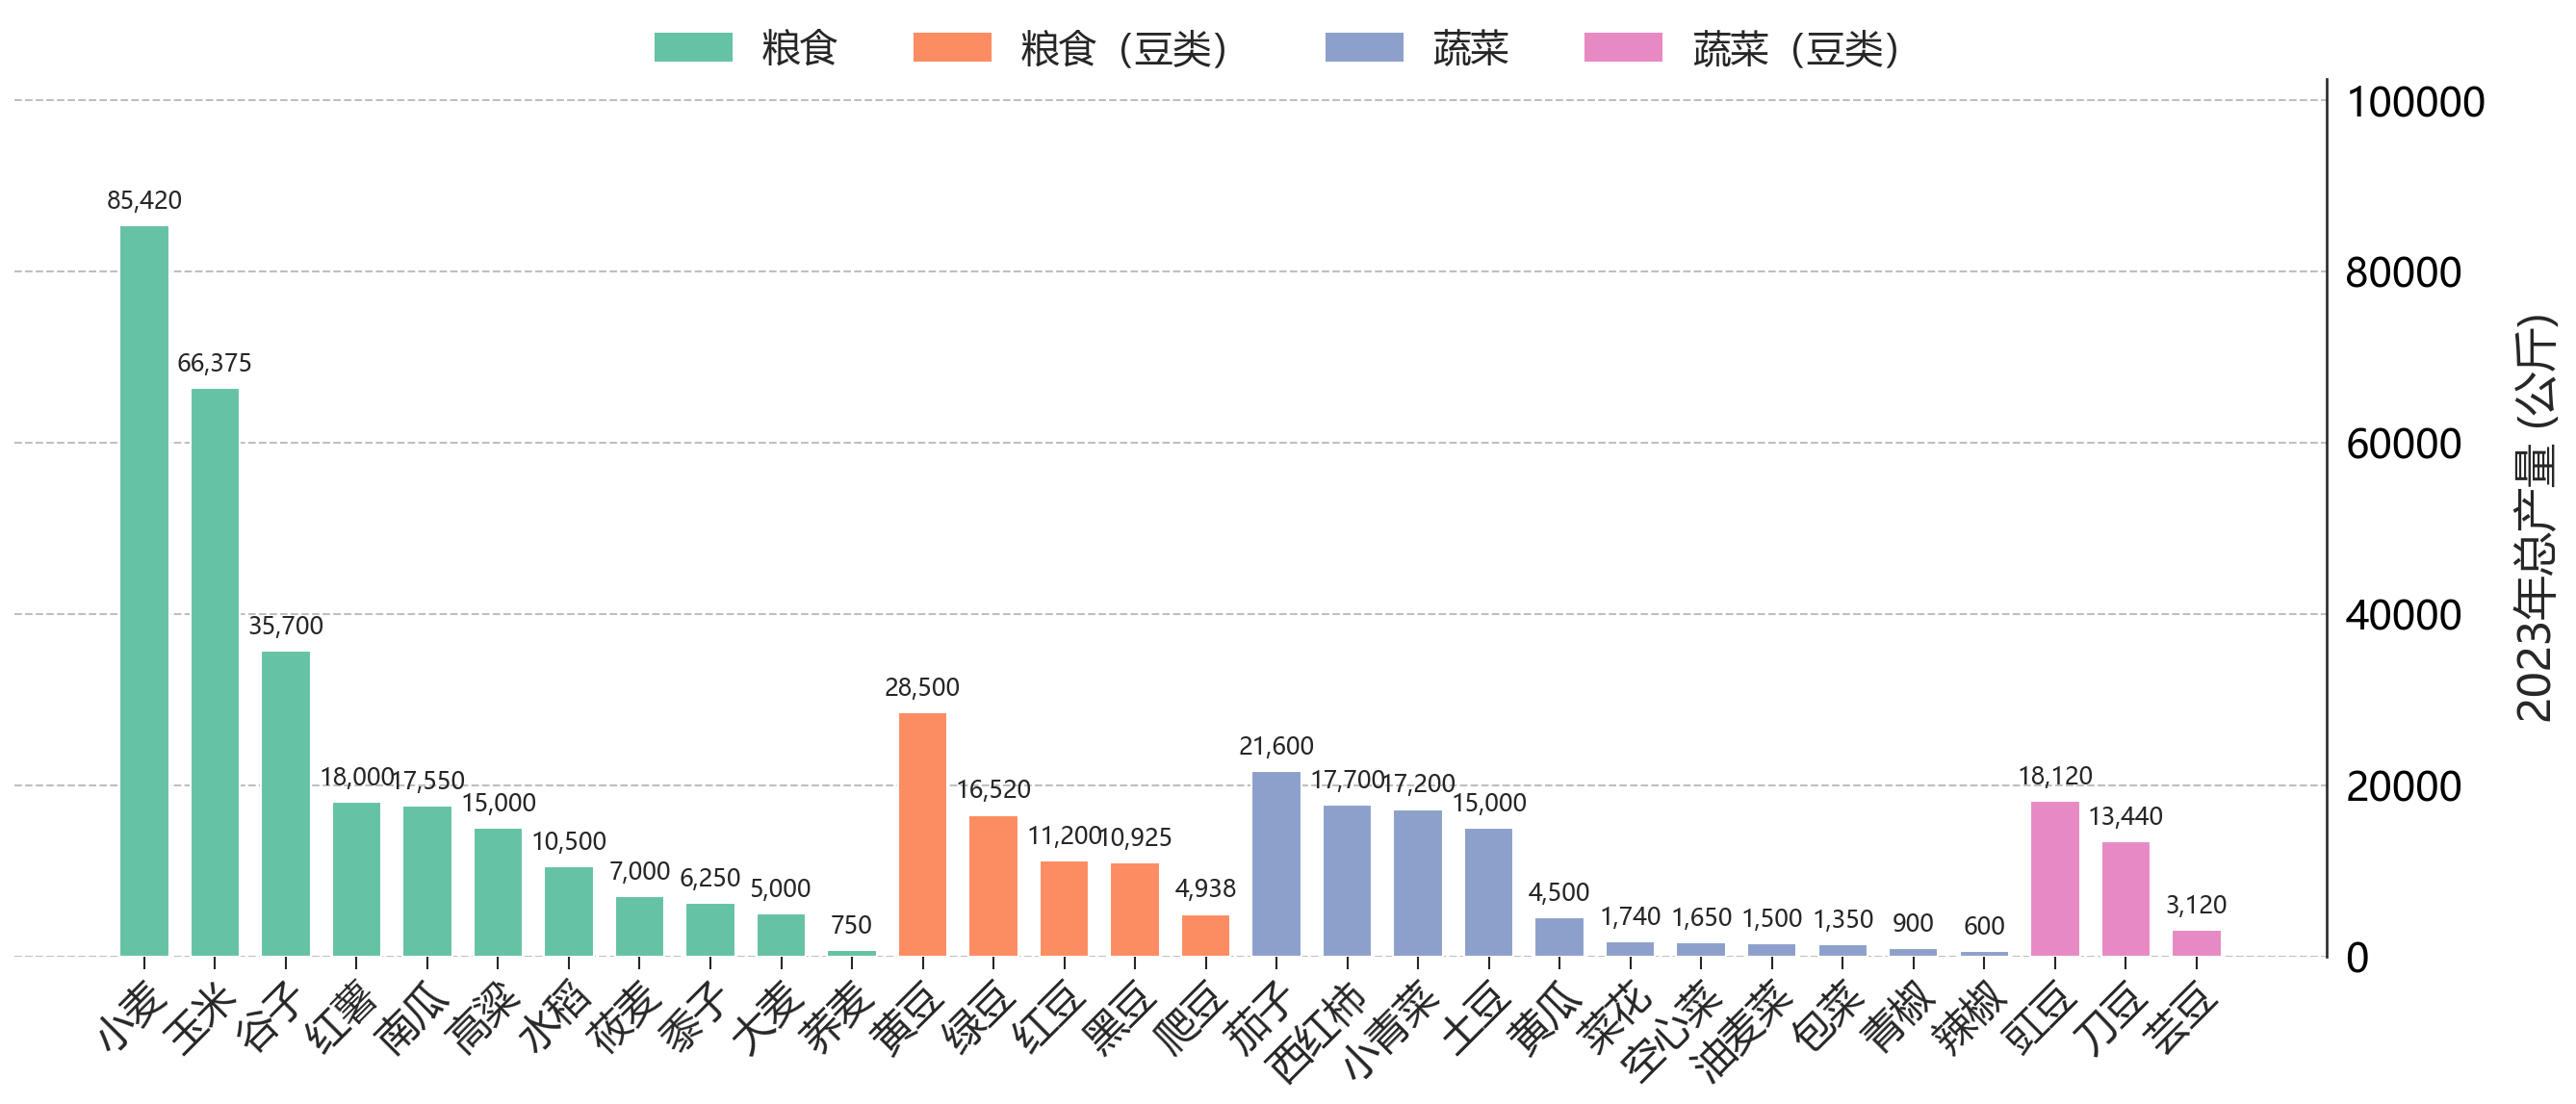
\includegraphics[width=0.8\textwidth]{figs/2数据分析与预处理/2023年产量分布.png}
    \caption{2023年农作物总产量分布}
    \label{fig:production_distribution_2023}
\end{figure}

图\ref{fig:profit_per_mu_2023}则揭示了不同作物在2023年的单位亩利润水平。单位面积的盈利能力是衡量作物经济价值的核心指标。

\begin{figure}[htbp]
    \centering
    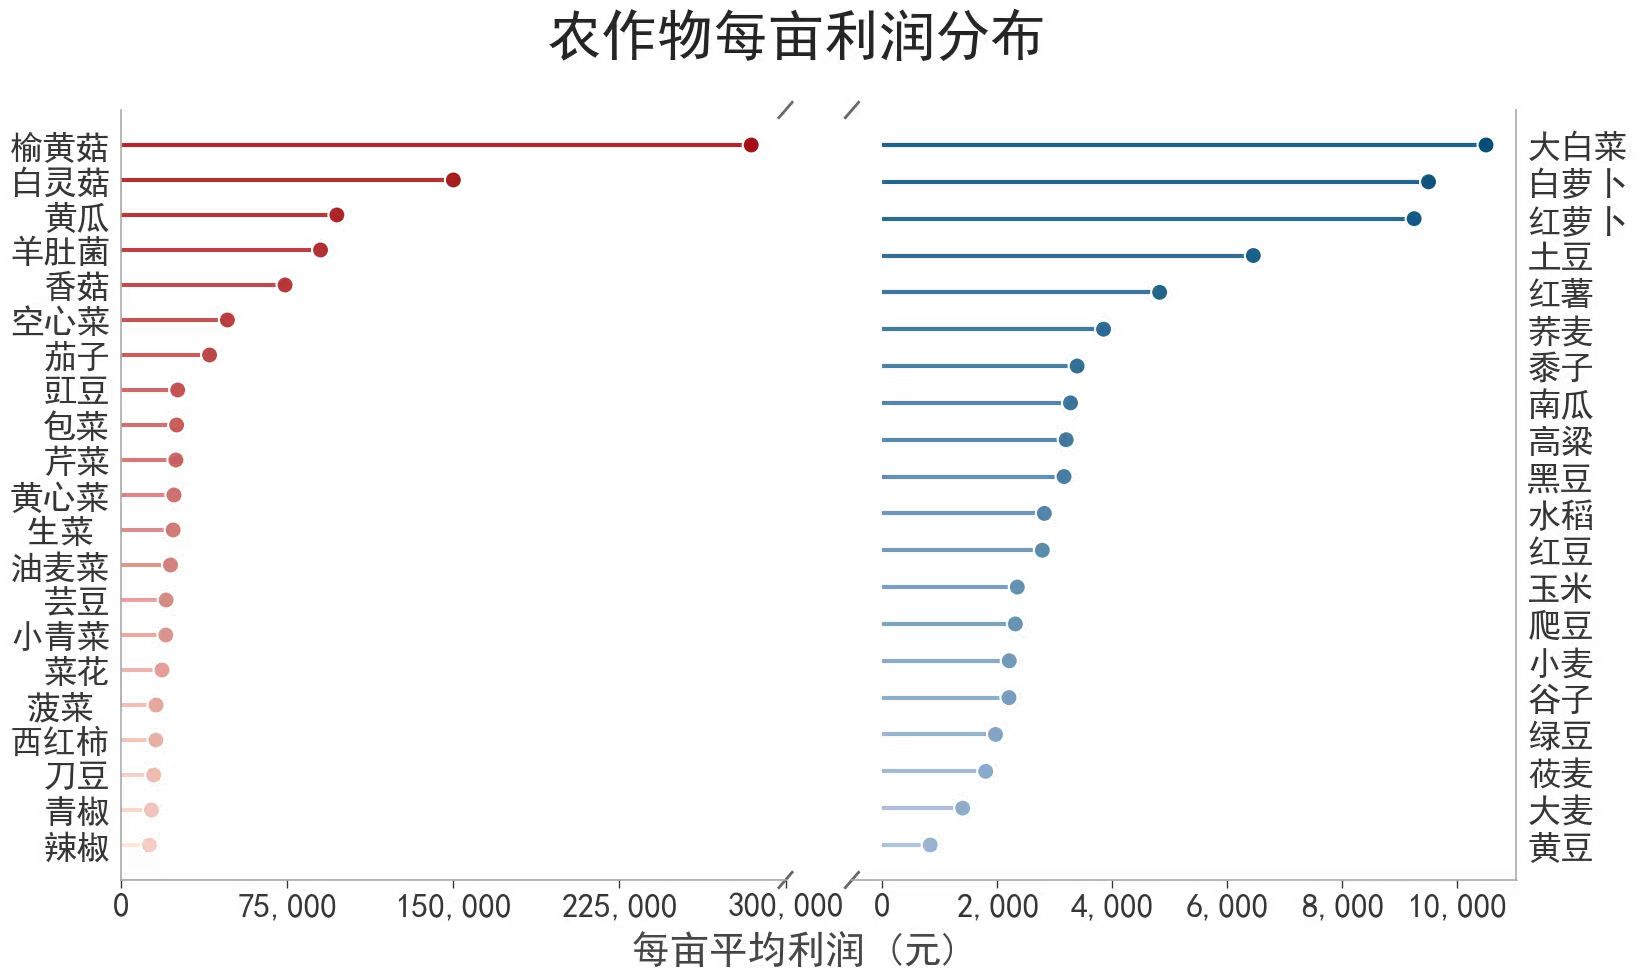
\includegraphics[width=0.8\textwidth]{figs/2数据分析与预处理/2023年单位亩利润}
    \caption{2023年各作物单位亩利润}
    \label{fig:profit_per_mu_2023}
\end{figure}

为统一衡量标准,我们将单位亩利润作为评估经济效益的基础。对于任意一种作物$i$,其单位亩利润$P_i$的计算方式如下:
\begin{equation}
    P_i = Y_i \times S_i - C_i
    \label{eq:profit}
\end{equation}
其中,$Y_i$表示作物$i$的单位亩产量(斤/亩),$S_i$表示其销售价格(元/斤),$C_i$表示其单位亩种植成本(元/亩)。通过此公式,我们将原始数据转化为直接用于优化模型目标函数的关键经济参数。

综上所述,通过对耕地资源、作物种植条件和经济效益指标的系统分析与处理,我们为后续构建多目标、多约束的种植策略优化模型奠定了坚实的数据基础。

% \section{问题一:风化影响分析与成分恢复模型}

古代玻璃文物在长期埋藏过程中会发生风化作用,导致其表面化学成分发生改变。为探究风化作用对不同类别玻璃文物的影响,并尝试恢复其风化前的成分含量,本章建立了分析与预测模型。我们首先检验了表面风化与文物其他物理属性之间的统计关联,然后分析了风化对高钾和铅钡两类玻璃化学成分含量的影响规律,最后构建了一个基于风化系数的预测模型,用于推断风化样品的原始化学成分,其框架如图\ref{fig:问题一模型框架}所示。

\begin{figure}[H]
	\centering
	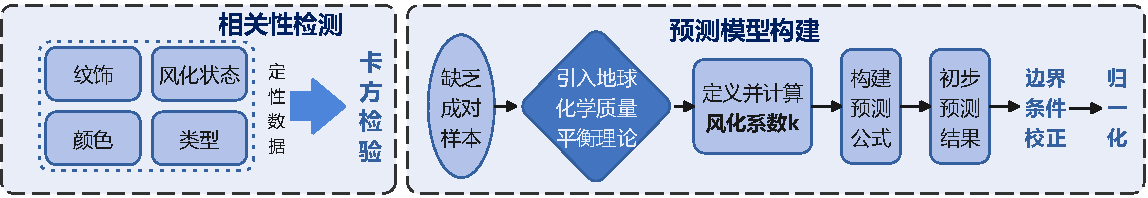
\includegraphics[width=\textwidth]{figs/3问题一/第一问框架.pdf}
	\caption{风化影响分析与成分恢复模型框架}
	\label{fig:问题一模型框架}
\end{figure}

\subsection{表面风化与文物物理属性的关联性检验}

为了探究文物表面风化现象是否与其物理属性存在关联,我们首先需要分析表面风化状态与玻璃类型、纹饰及颜色这几个变量之间的关系。这些变量的共同特征是它们均为分类变量,其取值为离散的类别而非连续的数值。

这一数据特性决定了用于衡量连续变量间线性关系的皮尔逊相关系数或用于比较组间均值差异的方差分析等方法在此并不适用,因为对“浅蓝”、“纹饰A”等类别进行数值运算不具备实际意义,需要采用一种能够处理定性数据频数的非参数检验方法来分析它们之间的关联性。因此,针对此问题,我们使用了卡方检验。

卡方检验是一种专门用于判断两个或多个分类变量之间是否存在关联的经典统计方法,其核心思想在于比较观测频数与期望频数之间的差异。其中,观测频数是样本数据中各类组合的实际计数值,而期望频数则是在“变量间相互独立”这一零假设下,根据边际概率计算出的理论计数值。检验过程通过计算两者差异的卡方统计量,并将其转换为$P$值来进行判断。在本研究中,我们设定显著性水平为$0.05$,若计算所得的$P$值小于该阈值,则拒绝变量间相互独立的零假设,认为它们之间存在显著的统计学关联。

为分析文物表面风化现象与其物理属性的关联,我们制作了关系分析的可视化图,如图\ref{fig:关系分析可视化}所示。图中第一部分展示了风化状态在两类玻璃中的分布情况。数据显示,铅钡玻璃的风化样本占其总数的73.5\%,这一比例远高于高钾玻璃的33.3\%。图中第二部分与第三部分则进一步展示了风化样本在不同纹饰和颜色类别下的数量分布。所有纹饰为B的样本均为风化样本,而纹饰为A的样本中风化与未风化数量相同。在不同颜色中,浅蓝色样本的风化数量为20,远超其未风化数量6,而蓝绿色样本中两者的数量则基本持平。这些在不同类别下风化比例与数量的显著差异直观地表明表面风化与文物的物理属性并非相互独立。





\begin{figure}[H]

\centering

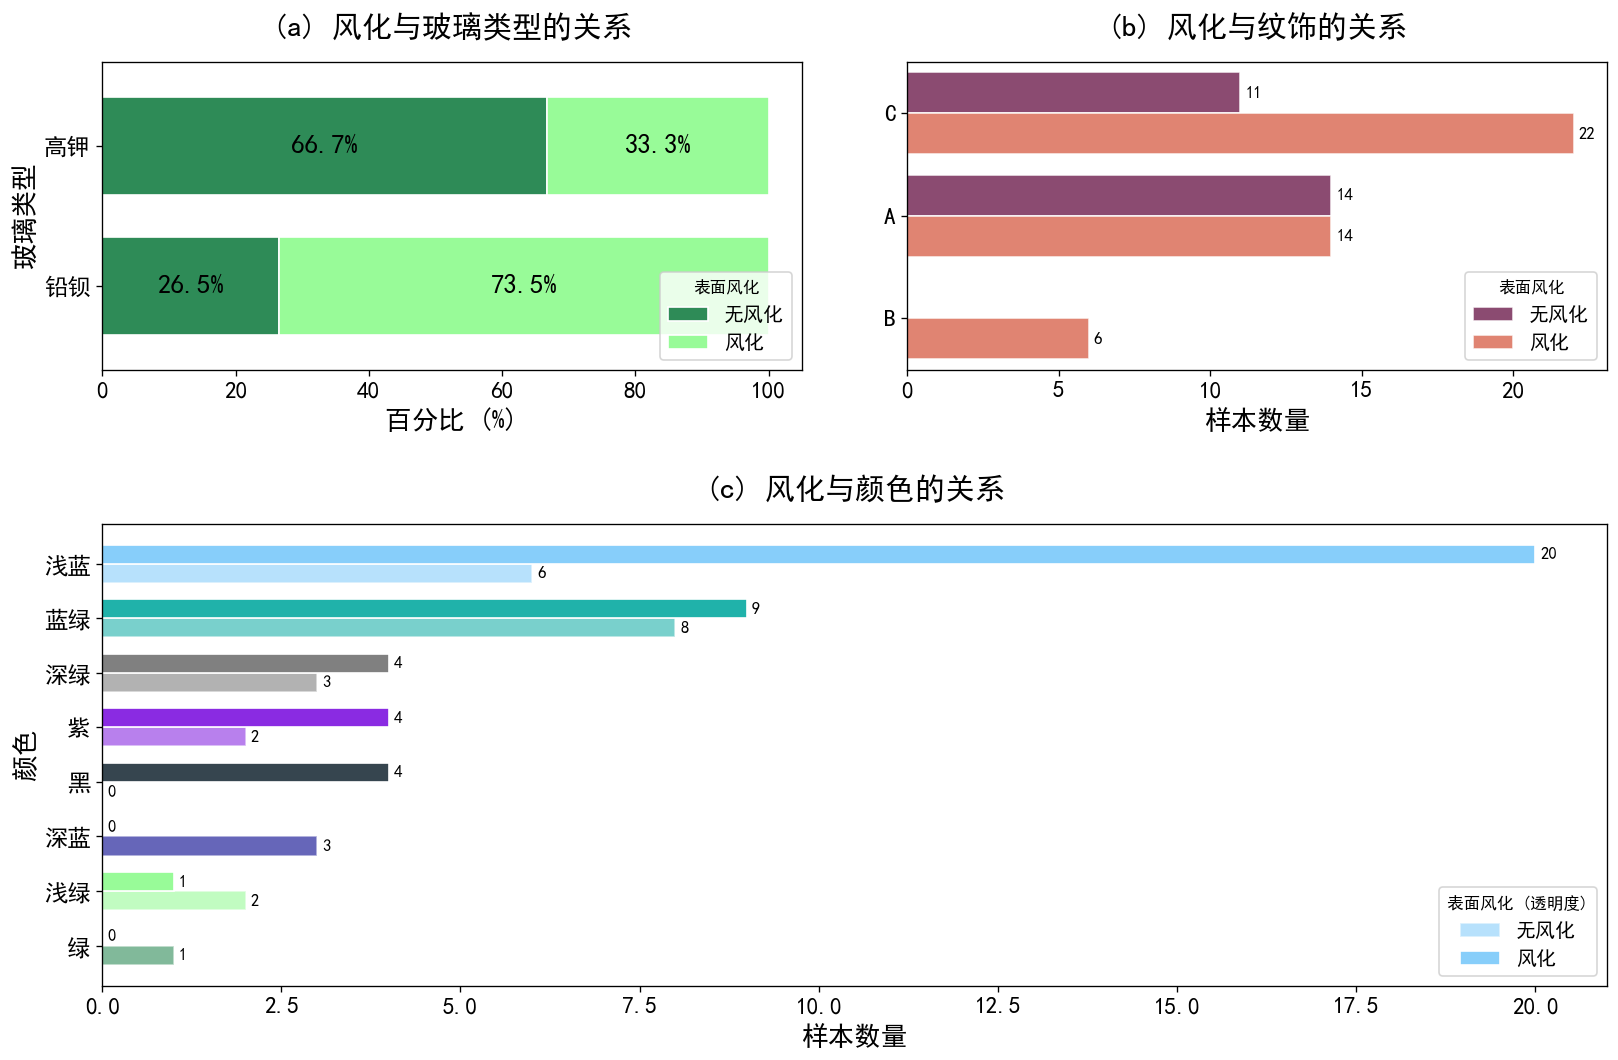
\includegraphics[width=\textwidth]{figs/3问题一/问题一_关系分析可视化_组合图_黄金分割.png}

\caption{表面风化与类型、纹饰及颜色的关系可视化}

\label{fig:关系分析可视化}

\end{figure}




\subsection{风化对两类玻璃化学成分含量的影响规律}

基于风化与玻璃类型存在关联的结论,我们进一步对风化在高钾和铅钡两类玻璃中引起的化学成分变化规律进行分析。我们将样本数据分为高钾未风化、高钾风化、铅钡未风化、铅钡风化四个组别,并对各组样本的化学成分含量分布进行了比较。

我们采用分面箱线图对两类玻璃在风化前后的化学成分分布进行可视化,如图\ref{fig:高钾玻璃成分分布}与图\ref{fig:铅钡玻璃成分分布}所示。箱线图展示了数据的中位数、四分位距和离散程度。从图中可以观察到,对于高钾玻璃,风化作用导致氧化钾$K_2O$的含量中位数显著下降,而氧化硅$SiO_2$的含量则有上升趋势。对于铅钡玻璃,风化作用主要表现为氧化铅$PbO$与氧化钡$BaO$含量的大幅降低,同时氧化硅$SiO_2$含量相应增加。这种变化说明风化过程中发生了元素的选择性流失与富集。

\begin{figure}[H]
	\centering
	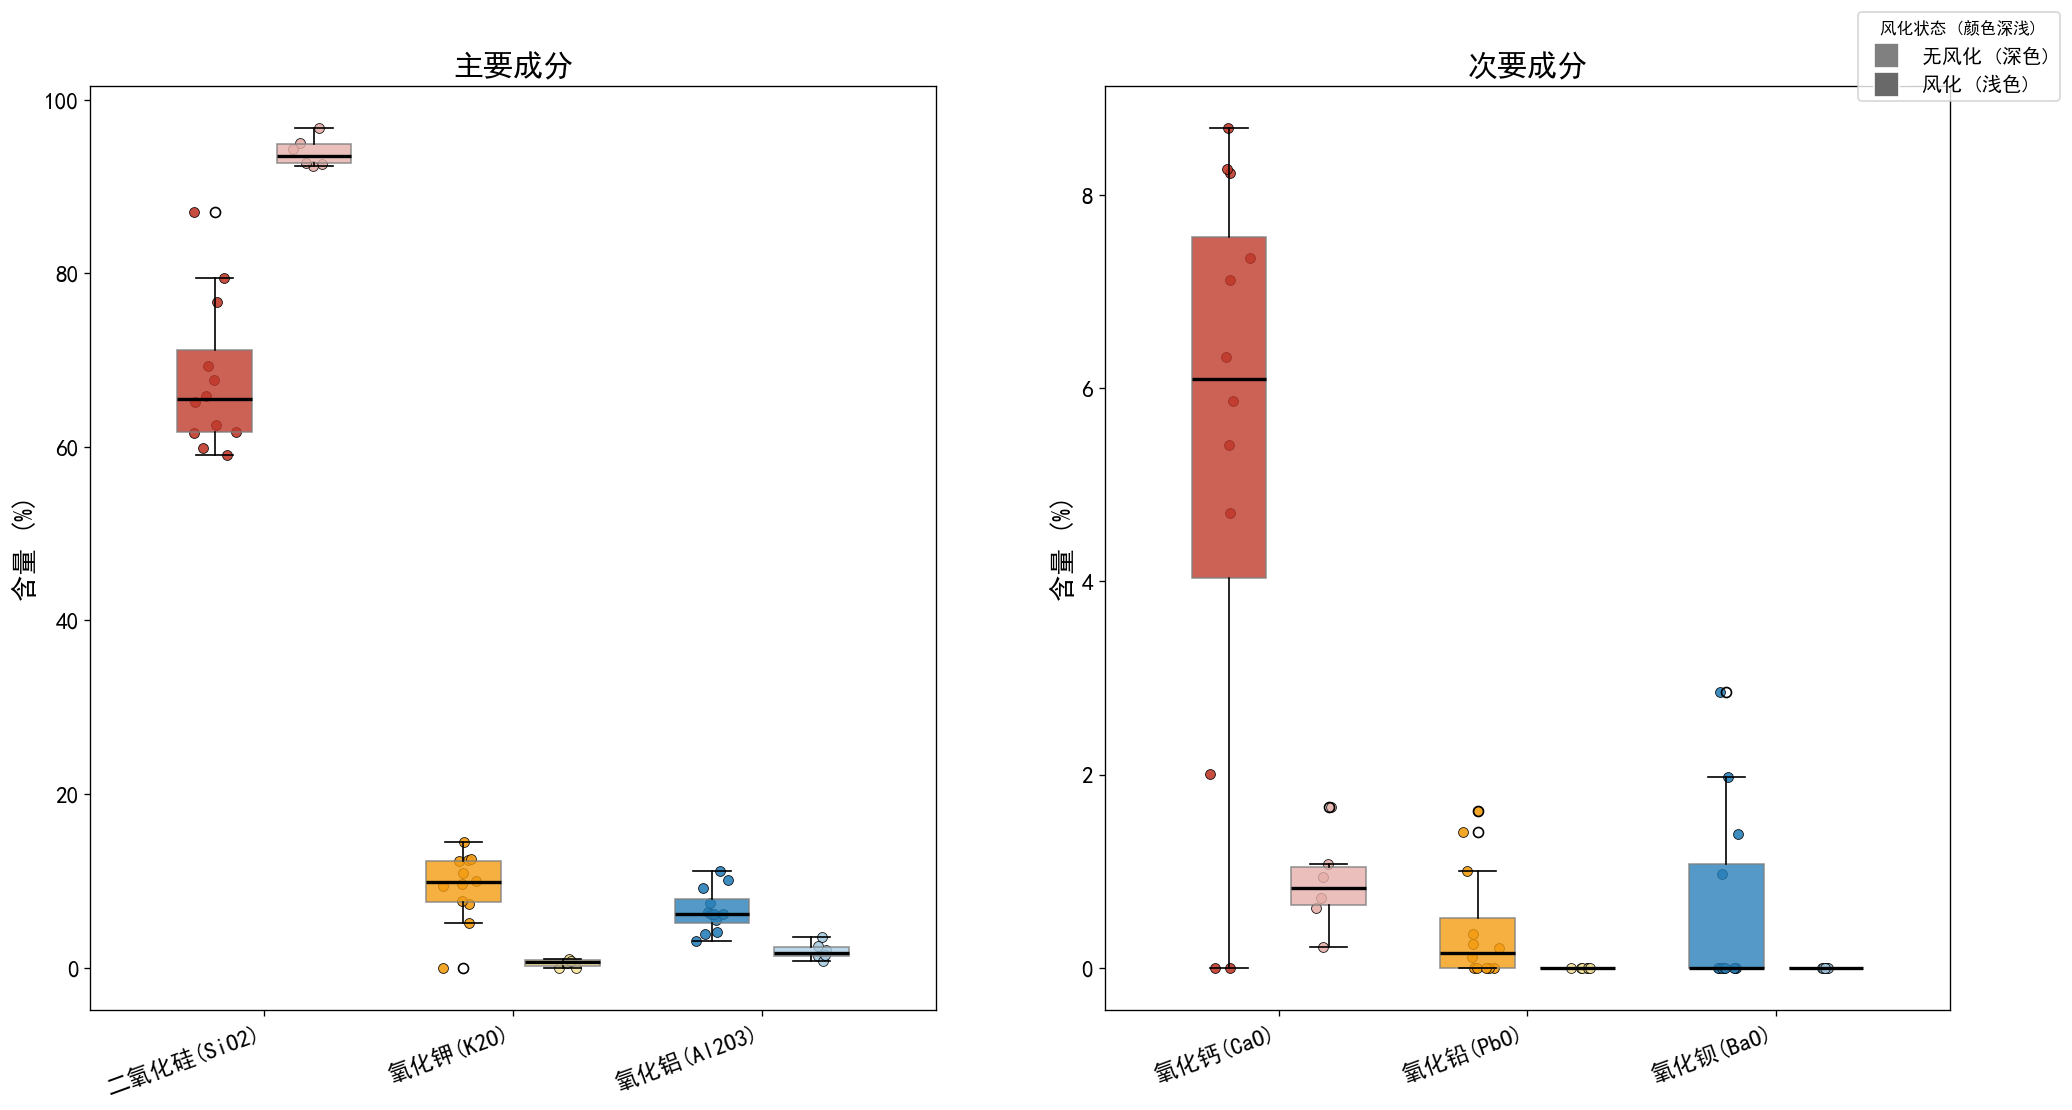
\includegraphics[width=\textwidth]{figs/3问题一/高钾玻璃成分分布.png}
	\caption{高钾玻璃在风化前后各化学成分含量分布}
	\label{fig:高钾玻璃成分分布}
\end{figure}

\begin{figure}[H]
	\centering
	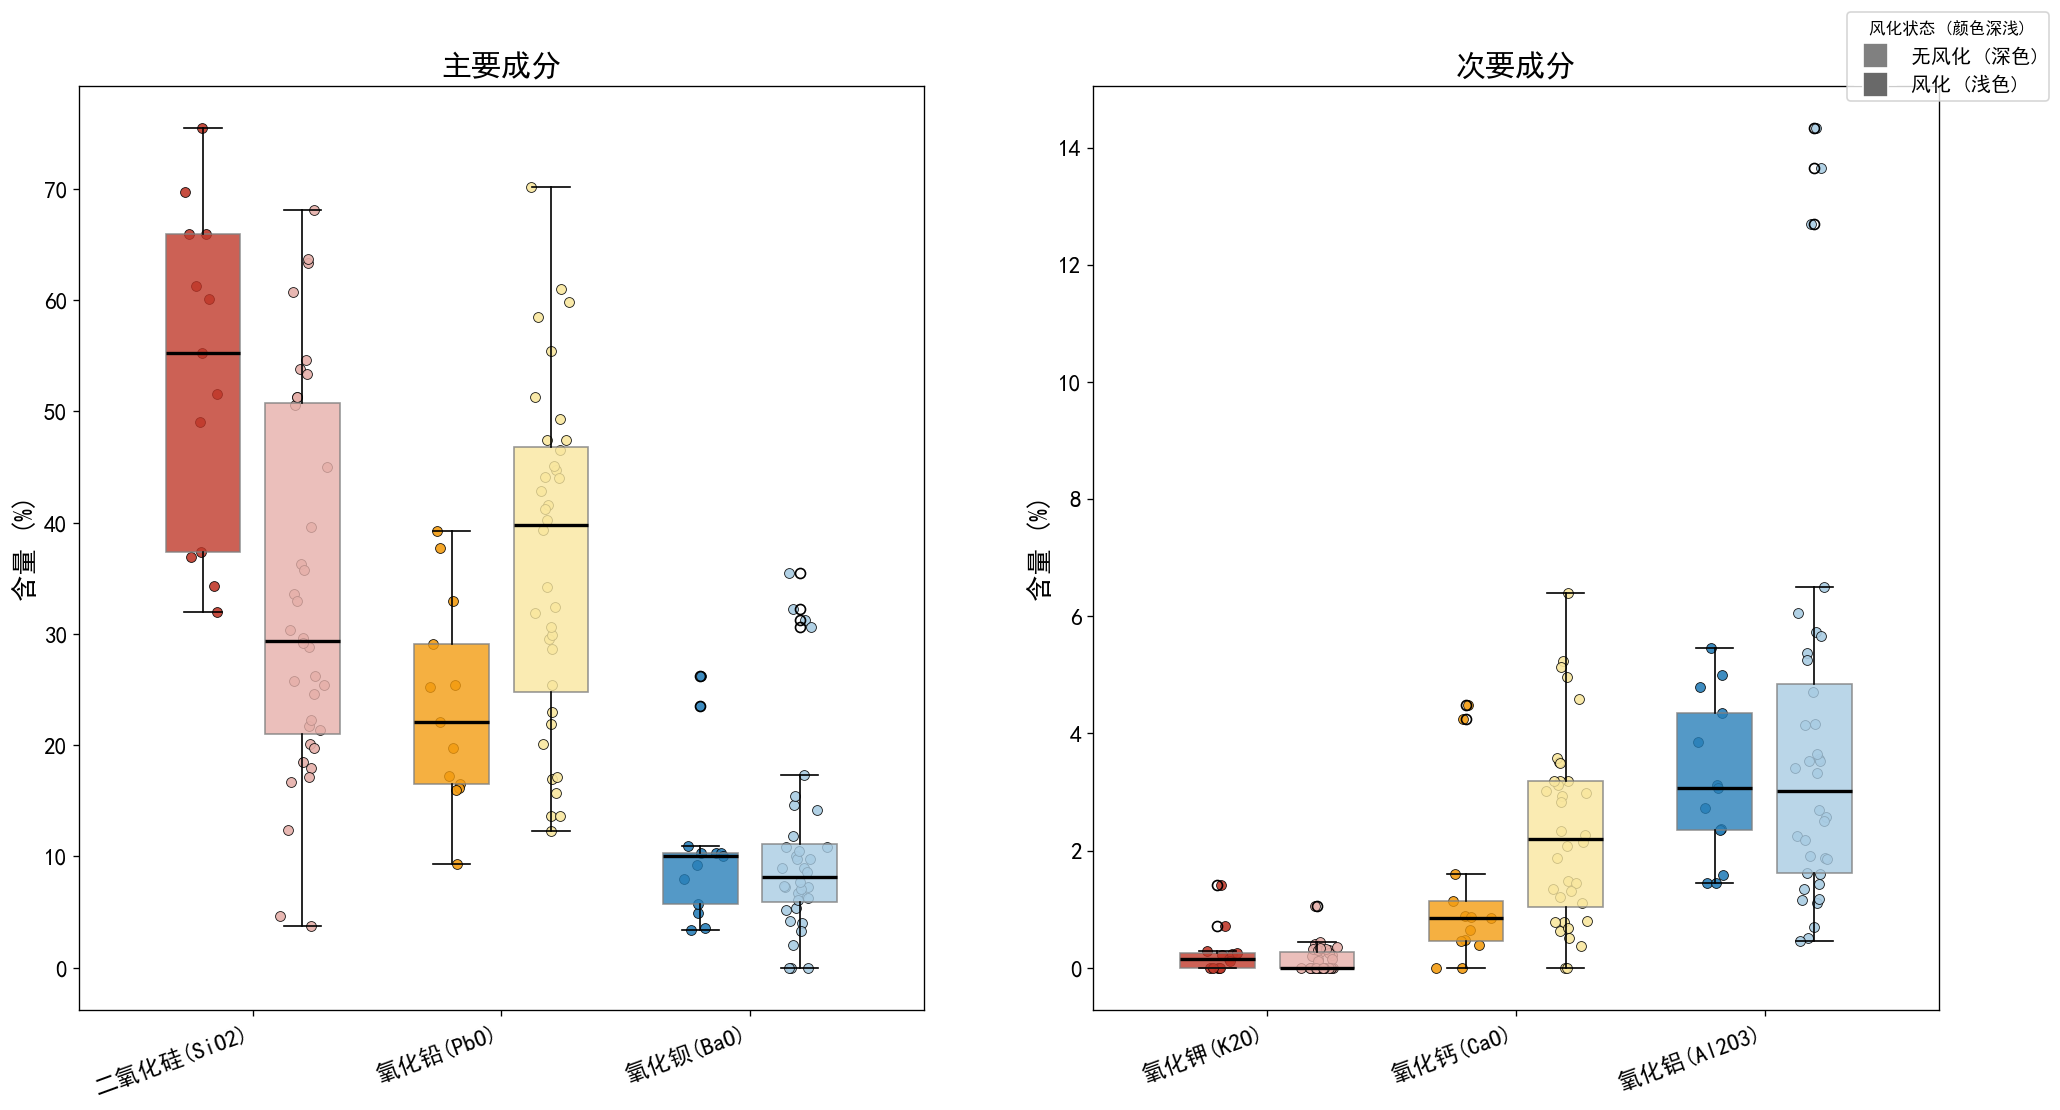
\includegraphics[width=\textwidth]{figs/3问题一/铅钡玻璃成分分布.png}
	\caption{铅钡玻璃在风化前后各化学成分含量分布}
	\label{fig:铅钡玻璃成分分布}
\end{figure}


为了更细致地观察关键化学成分的分布形态变化,我们绘制了部分核心化学成分,包括氧化铅$PbO$、氧化钾$K_2O$、氧化钡$BaO$以及二氧化硅$SiO_2$的分布图,如图\ref{fig:pbo_dist}至图\ref{fig:sio2_dist}所示。图中包含直方图与核密度估计曲线,它们共同描述了数据分布的集中趋势和形态。分析这些分布图可以发现,高钾玻璃在风化后,其氧化钾$K_2O$的含量分布从一个较宽的区间转化至接近零值的极低水平。对于铅钡玻璃,风化作用使其特征成分氧化铅$PbO$与氧化钡$BaO$的含量分布整体向低值区移动。与此相反,作为玻璃基体的二氧化硅$SiO_2$,其含量分布在两类玻璃中均表现出向高值区偏移的趋势,说明在风化过程中其他元素的流失导致了二氧化硅的相对富集。


\begin{figure}[H]
	\centering
	\begin{minipage}{0.48\textwidth}
		\centering
		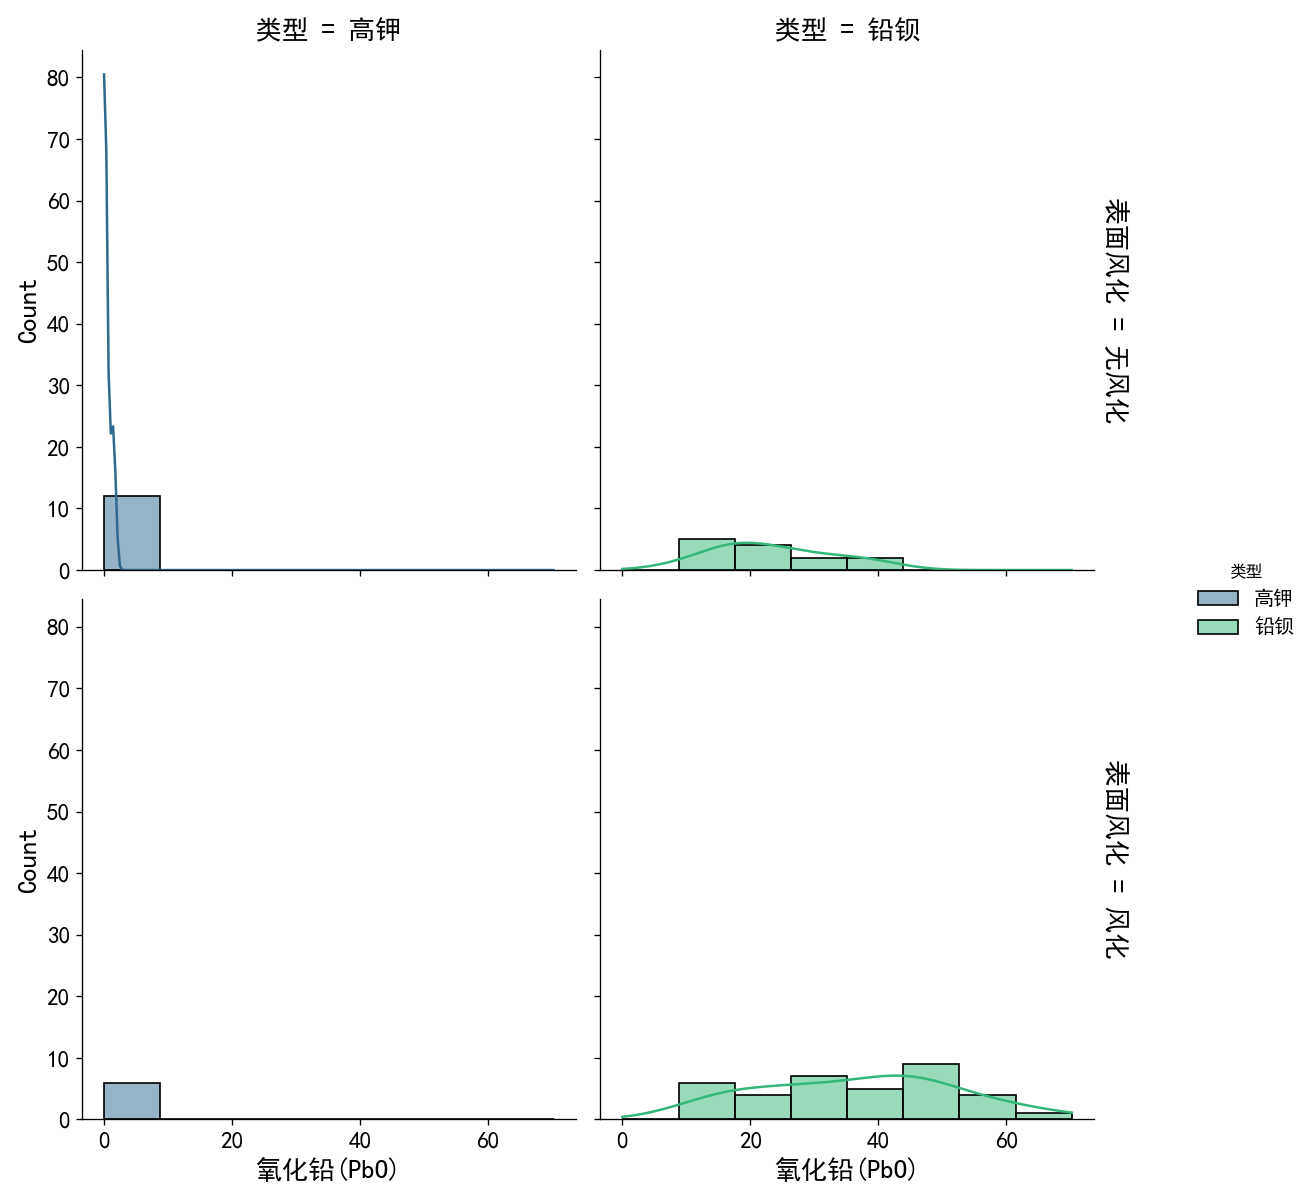
\includegraphics[width=\linewidth]{figs/3问题一/分布图_氧化铅(PbO).png}
		\caption{氧化铅$PbO$含量分布}
		\label{fig:pbo_dist}
	\end{minipage}\hfill
	\begin{minipage}{0.48\textwidth}
		\centering
		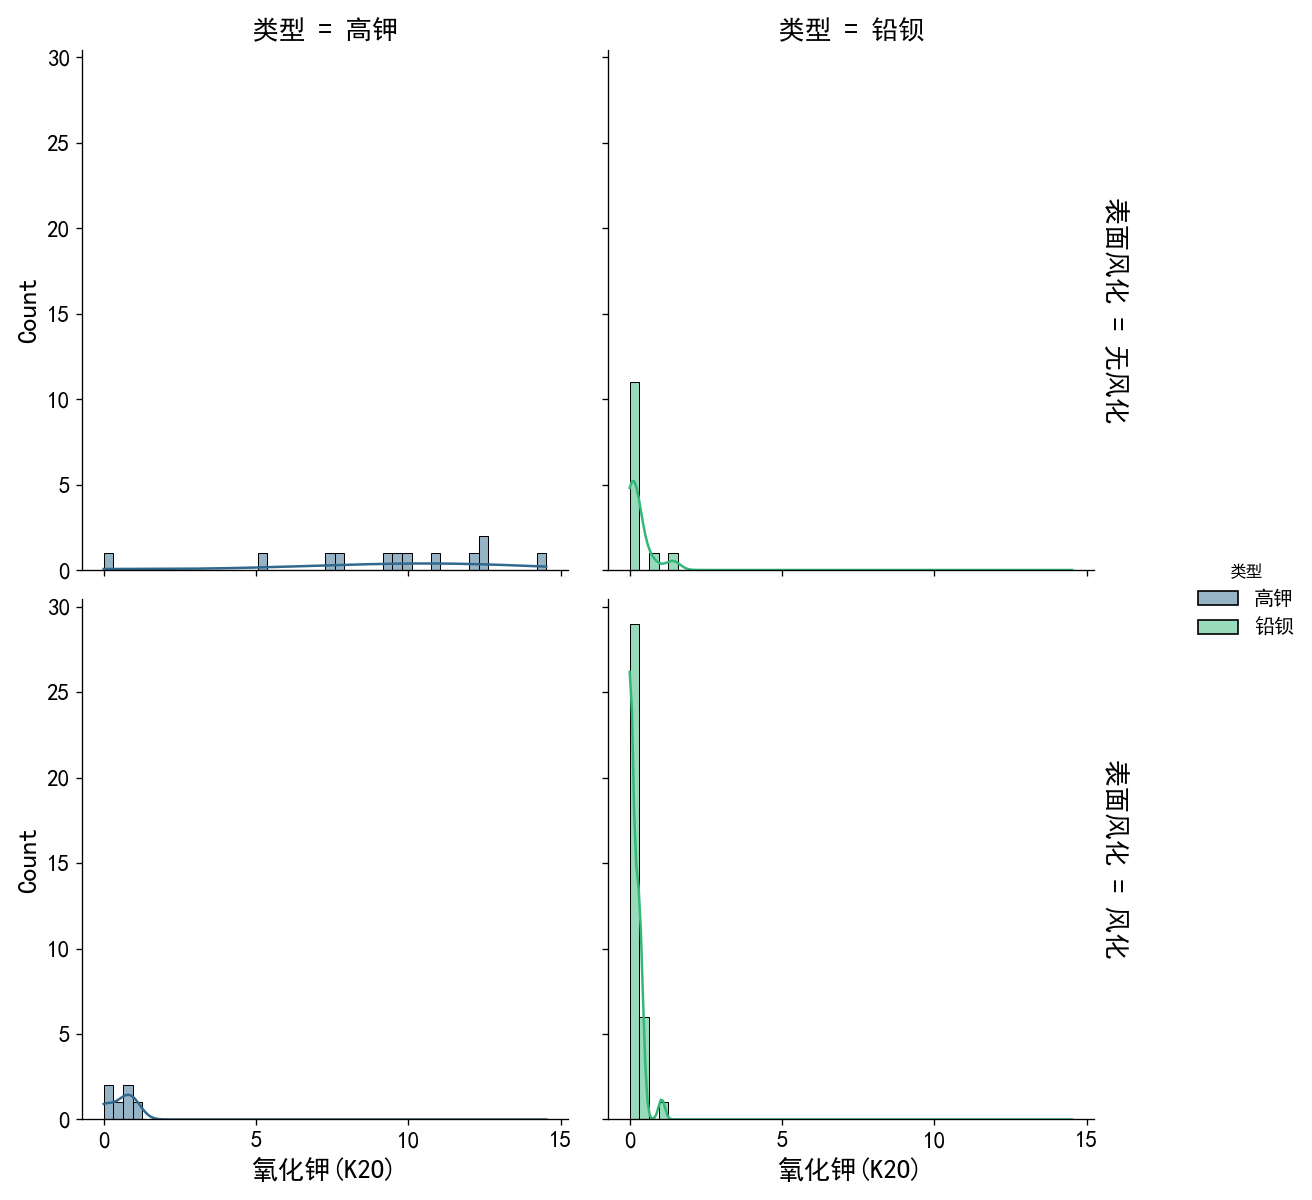
\includegraphics[width=\linewidth]{figs/3问题一/分布图_氧化钾(K2O).png}
		\caption{氧化钾$K_2O$含量分布}
		\label{fig:k2o_dist}
	\end{minipage}
\end{figure}

\begin{figure}[H]
	\centering
	\begin{minipage}{0.48\textwidth}
		\centering
		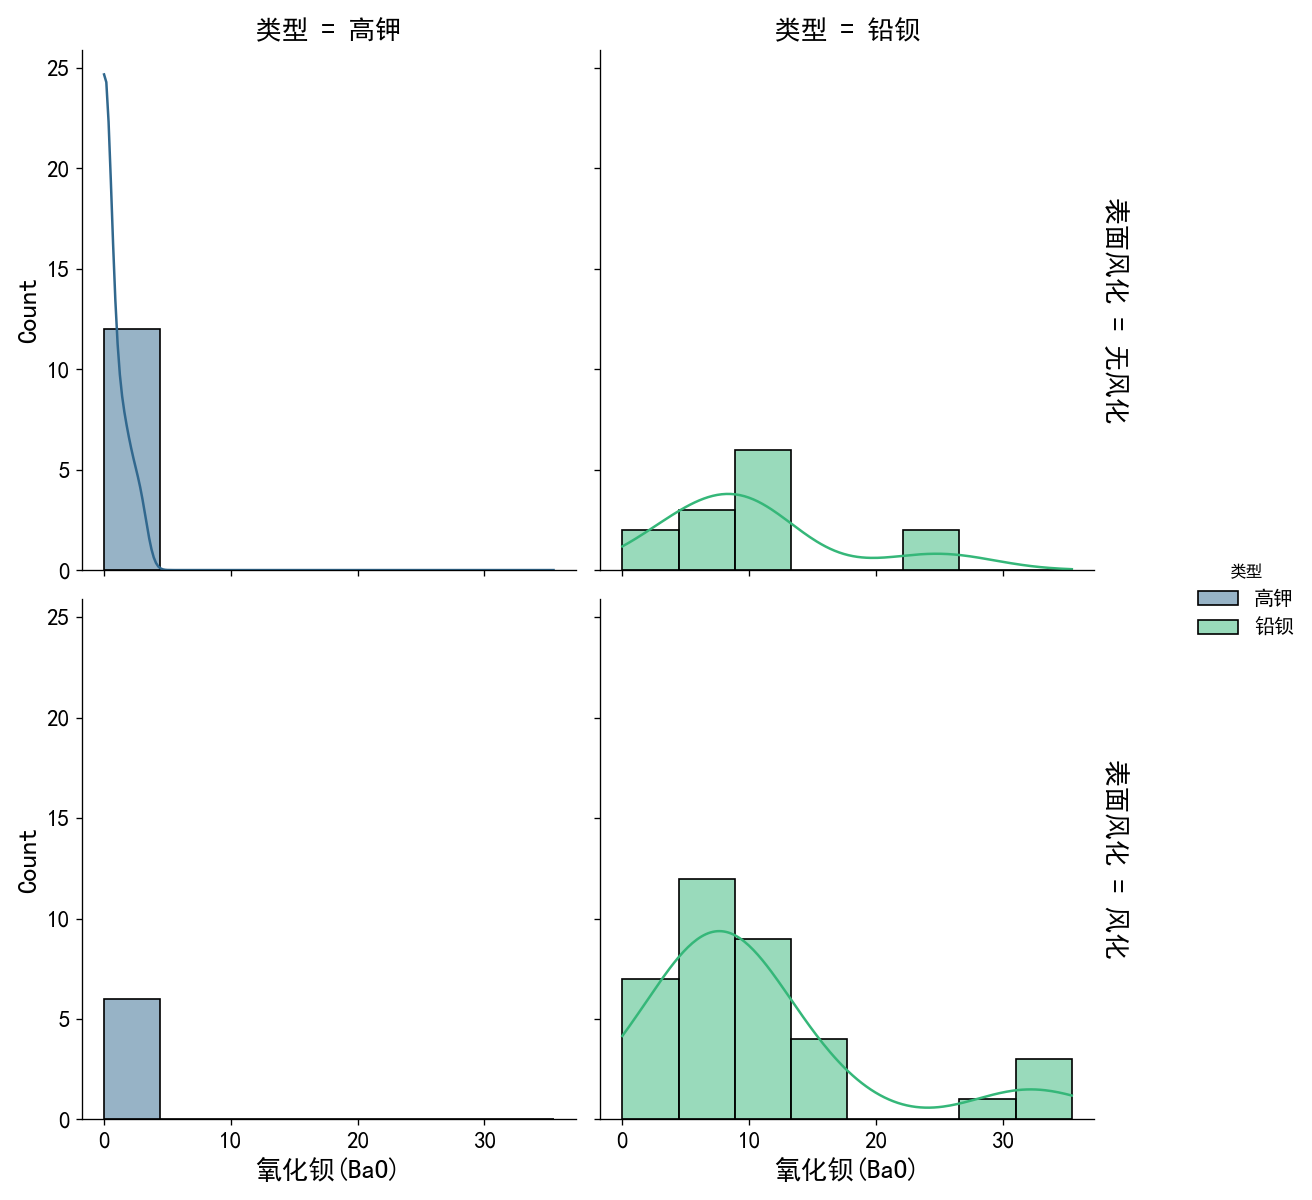
\includegraphics[width=\linewidth]{figs/3问题一/分布图_氧化钡(BaO).png}
		\caption{氧化钡$BaO$含量分布}
		\label{fig:bao_dist}
	\end{minipage}\hfill
	\begin{minipage}{0.48\textwidth}
		\centering
		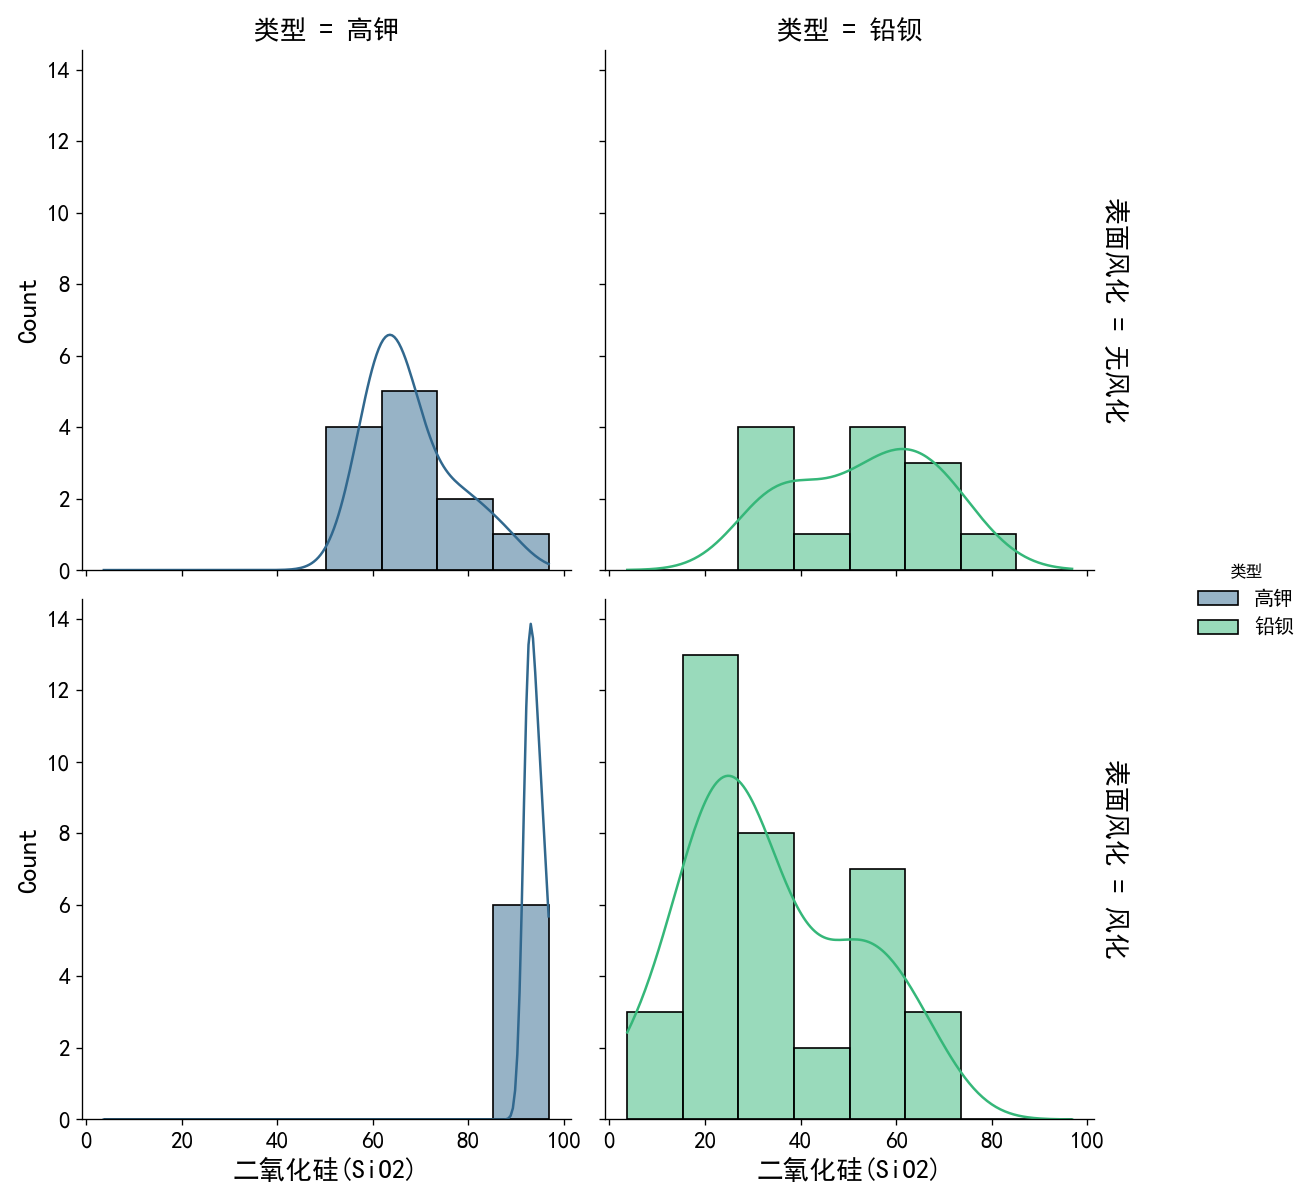
\includegraphics[width=\linewidth]{figs/3问题一/分布图_二氧化硅(SiO2).png}
		\caption{二氧化硅$SiO_2$含量分布}
		\label{fig:sio2_dist}
	\end{minipage}
\end{figure}

\subsection{基于风化系数的化学成分含量预测模型}

预测风化前化学成分的主要困难在于数据中缺乏源自同一文物的风化与未风化的观测样本。这使得依赖大量成对样本进行训练的传统监督学习模型,例如回归分析,难以直接应用且存在较高的过拟合风险。

于是,我们转向从风化过程的物理化学机理中寻求建模依据。玻璃的风化过程与地质学中岩石的蚀变过程在原理上具有相似性,均为长期化学环境作用下的元素迁移过程。因此,我们引入了地球化学领域成熟的质量平衡分析理论来构建预测模型,该理论能够在缺乏直接演变过程数据时,对成分变化进行有效推断。

我们的模型的核心假设为:特定化学成分在风化过程中的流失或富集比例,与其在未风化状态下的原始含量相关。此假设参考了地质学中分析交代蚀变作用的艾索康图法的原理,它将风化视为一个系统性的化学变化过程而非随机过程,从而建立了基于风化系数的预测方法。

我们首先为每种玻璃类型$t$和每种化学成分$j$定义一个风化系数$k_{t,j}$。该系数由该类型玻璃中所有风化样本与未风化样本的平均含量计算得出,其数学表达式如下:
\begin{equation}
	k_{t,j} = 1 - \frac{\bar{C}_{t,j,\text{weathered}}}{\bar{C}_{t,j,\text{unweathered}}}
\end{equation}
其中,$\bar{C}_{t,j,\text{weathered}}$表示$t$类玻璃风化样本中$j$成分的平均含量,$\bar{C}_{t,j,\text{unweathered}}$表示$t$类玻璃未风化样本中$j$成分的平均含量。

利用计算得到的风化系数,我们可以对任意一个已知风化后成分含量$C_{\text{weathered}, j}$的样本,进行其风化前含量$C'_{\text{unweathered}, j}$的初步预测,其预测公式为:
\begin{equation}
	C'_{\text{unweathered}, j} = \frac{C_{\text{weathered}, j}}{1 - k_{t,j}}
\end{equation}

考虑到测量误差和模型的局限性,初步预测得到的各成分总和可能偏离100\%。因此,我们对预测结果进行了边界条件校正。我们计算所有预测成分的总和,并进行条件归一化处理,以确保最终得到的预测成分总和落入题目要求的85\%至105\%的有效区间内,从而使预测结果在化学上更具合理性。模型的最终预测结果,以原始含量和预测含量并列对比的形式,被完整地保存至\texttt{Result/问题一\_预测结果.xlsx}文件中。


% \section{问题二:玻璃文物分类、亚类划分及可靠性分析}

本部分的目标是根据文物的化学成分,建立高钾玻璃与铅钡玻璃的分类规律,并对两类玻璃进行内部亚类的划分,最后对所得结论的可靠性进行系统性分析。其框架如图\ref{fig:problem2_framework}所示。

\begin{figure}[H]
    \centering
    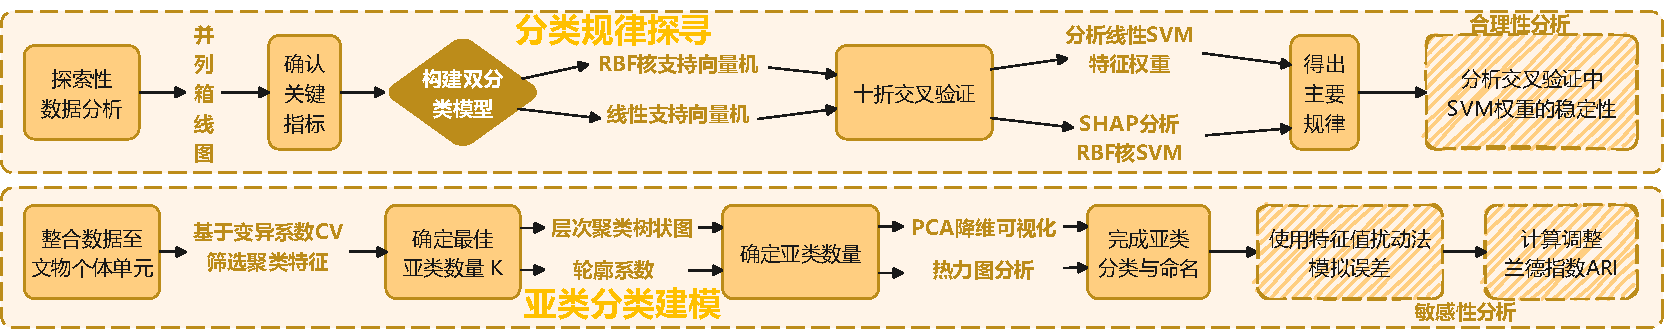
\includegraphics[width=\textwidth]{figs/4问题二/第二问框架.pdf}
    \caption{问题二框架}
    \label{fig:problem2_framework}
\end{figure}

\subsection{高钾玻璃与铅钡玻璃的分类规律}

在构建分类模型之前,首先需要通过探索性数据分析对不同类别的数据在数值特征上的分布差异建立直观认知,这为后续的建模方向和假设形成提供依据。我们采用并列箱线图来直观对比高钾玻璃与铅钡玻璃在全部十四种化学成分含量上的分布差异。

\begin{figure}[H]
    \centering
    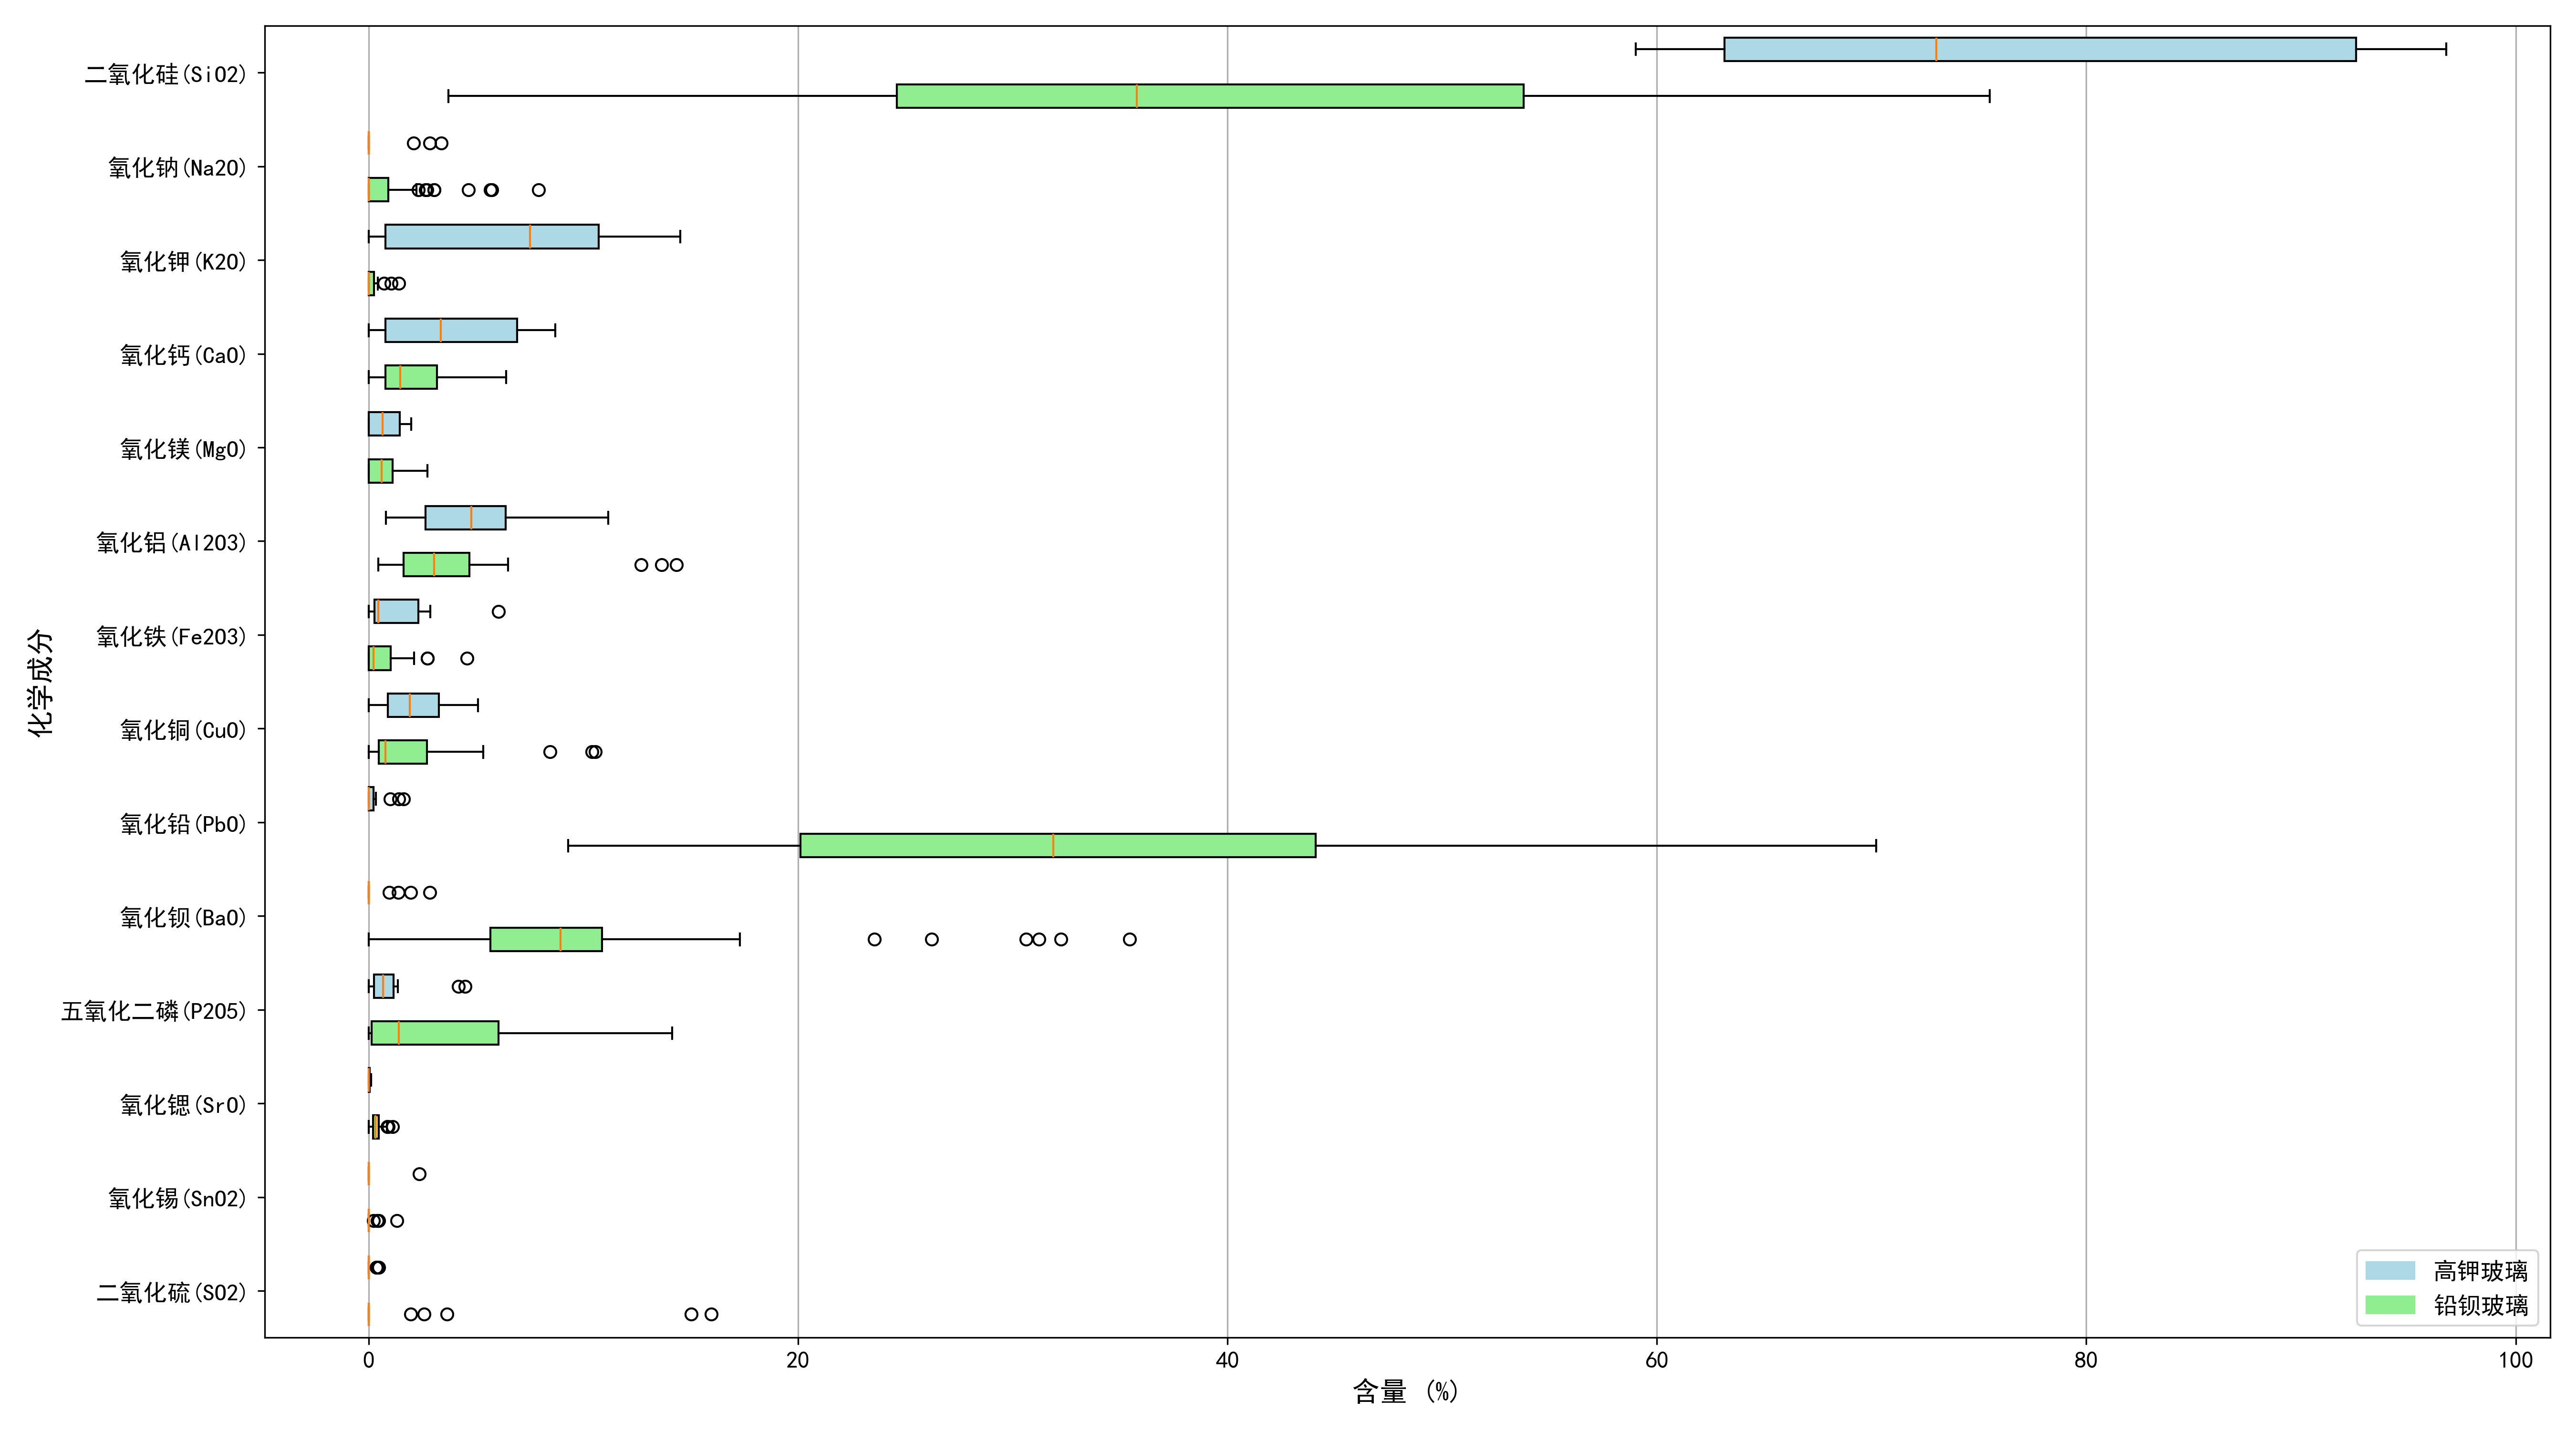
\includegraphics[width=\textwidth]{figs/4问题二/EDA_并列箱线图.png}
    \caption{高钾玻璃与铅钡玻璃化学成分含量分布对比}
    \label{fig:eda_boxplot}
\end{figure}

如图\ref{fig:eda_boxplot}所示,图中纵轴为化学成分,横轴为含量百分比。对于每一种成分,均并排展示了两个箱体,分别代表高钾玻璃和铅钡玻璃的含量分布。由图可知,在氧化铅$PbO$与氧化钡$BaO$两种成分上,铅钡玻璃的含量分布远高于高钾玻璃,而在氧化钾$K_2O$上则呈现相反的模式。两个类别在这些关键成分上的分布区间几乎没有重叠,由此形成核心假设,即$PbO$、$BaO$与$K_2O$是区分两类玻璃的关键指标。

基于前述探索性分析形成的假设,即特定化学成分含量可有效区分玻璃类型,我们构建监督学习分类模型以对该规律进行量化验证。为兼顾模型的解释性与对数据复杂关系的拟合能力,我们分别建立了线性支持向量机与使用径向基函数核的非线性支持向量机模型。

线性支持向量机的基本原理是在一个多维特征空间中,寻找一个最优的分类超平面。该超平面由法向量$\boldsymbol{w}$和位移$b$定义,其数学形式为$\boldsymbol{w}^T\boldsymbol{x} + b = 0$。最优化的目标是不仅能将两类样本分开,同时能最大化距离超平面最近的样本,即支持向量,到超平面的间隔。在允许部分样本被错误分类以增强模型泛化能力的情况下,该问题可表述为一个软间隔优化问题,其目标函数如下
\begin{equation}
    \min_{\boldsymbol{w}, b, \boldsymbol{\xi}} \frac{1}{2} ||\boldsymbol{w}||^2 + C \sum_{i=1}^{m} \xi_i
\end{equation}
式中$C$为正则化系数,用于平衡间隔最大化与分类误差,$\xi_i$是松弛变量,允许样本点在一定程度上偏离其正确的分类边界。

当化学成分与玻璃类型的关系无法通过线性边界有效分离时,需要引入非线性模型。非线性支持向量机通过核技巧将原始特征空间映射到一个更高维度的空间,并在新空间中构造线性超平面。我们选用径向基函数核,即高斯核,作为映射函数,其定义为
\begin{equation}
    K(\boldsymbol{x}_i, \boldsymbol{x}_j) = \exp(-\gamma ||\boldsymbol{x}_i - \boldsymbol{x}_j||^2)
\end{equation}
其中$\gamma$是核函数的一个参数,它决定了单个训练样本影响范围的大小。通过使用该核函数,模型能够在原始空间中形成复杂的非线性决策边界。

为获得稳健的模型性能评估,避免因单次数据划分带来的偶然性,我们采用十折交叉验证方法。该方法将数据集随机分为十个互斥的子集,轮流使用其中九个作为训练集,一个作为测试集,最终以十次测试结果的平均值作为模型的性能度量。评估结果显示,线性支持向量机模型的平均分类准确率为95.71\%,而使用径向基函数核的非线性支持向量机模型平均分类准确率达到97.41\%。两个模型均表现出较高的分类能力。

为解释模型的分类机理,我们首先分析了线性支持向量机学习到的特征权重。

\begin{figure}[H]
    \centering
    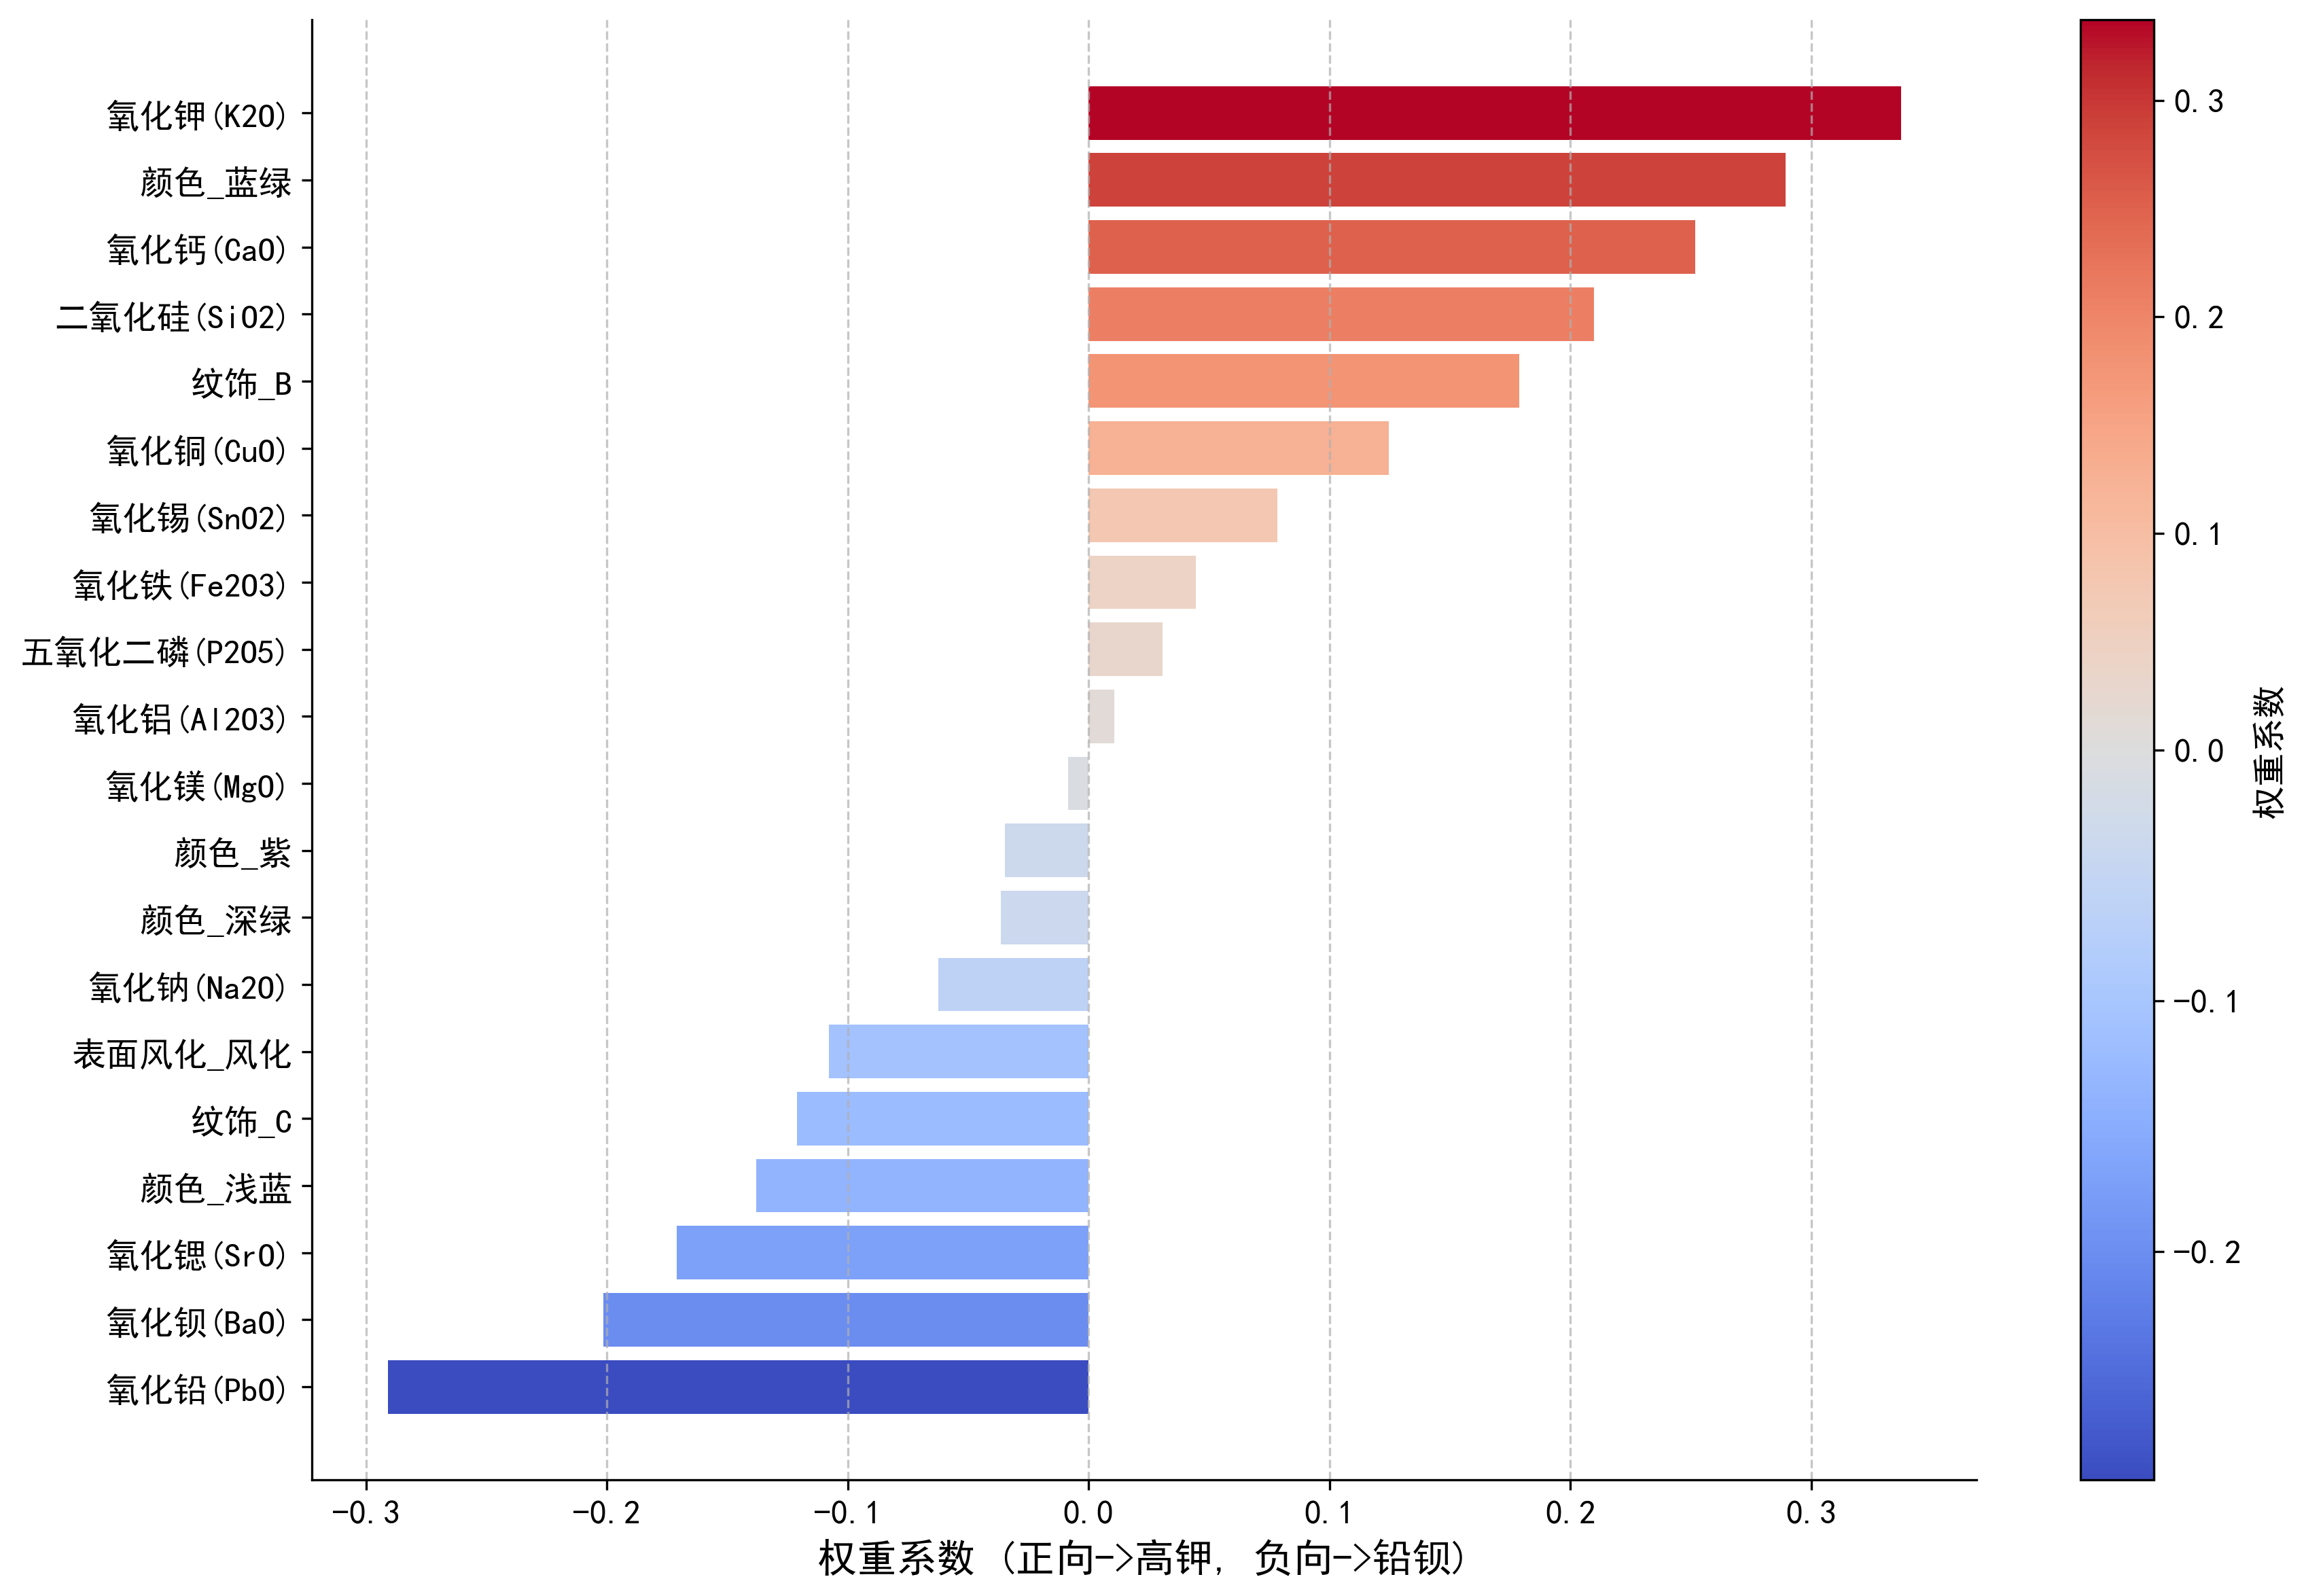
\includegraphics[width=\textwidth]{figs/4问题二/线性SVM特征权重_渐变色.png}
    \caption{线性支持向量机模型学习的特征权重}
    \label{fig:svm_weights}
\end{figure}

图\ref{fig:svm_weights}展示了各化学成分的权重系数值,其中正向权重将预测推向高钾玻璃,负向权重则推向铅钡玻璃。图中可见,氧化钾$K_2O$与二氧化硅$SiO_2$获得了最大的正权重,而氧化铅$PbO$与氧化钡$BaO$获得了最大的负权重,这与探索性分析的发现一致。

对于性能更高但解释性较弱的非线性模型,我们采用SHAP,即SHapley Additive exPlanations框架进行分析。该方法基于合作博弈论,能够将模型的预测结果公平地归因到每个输入特征上。

\begin{figure}[H]
    \centering
    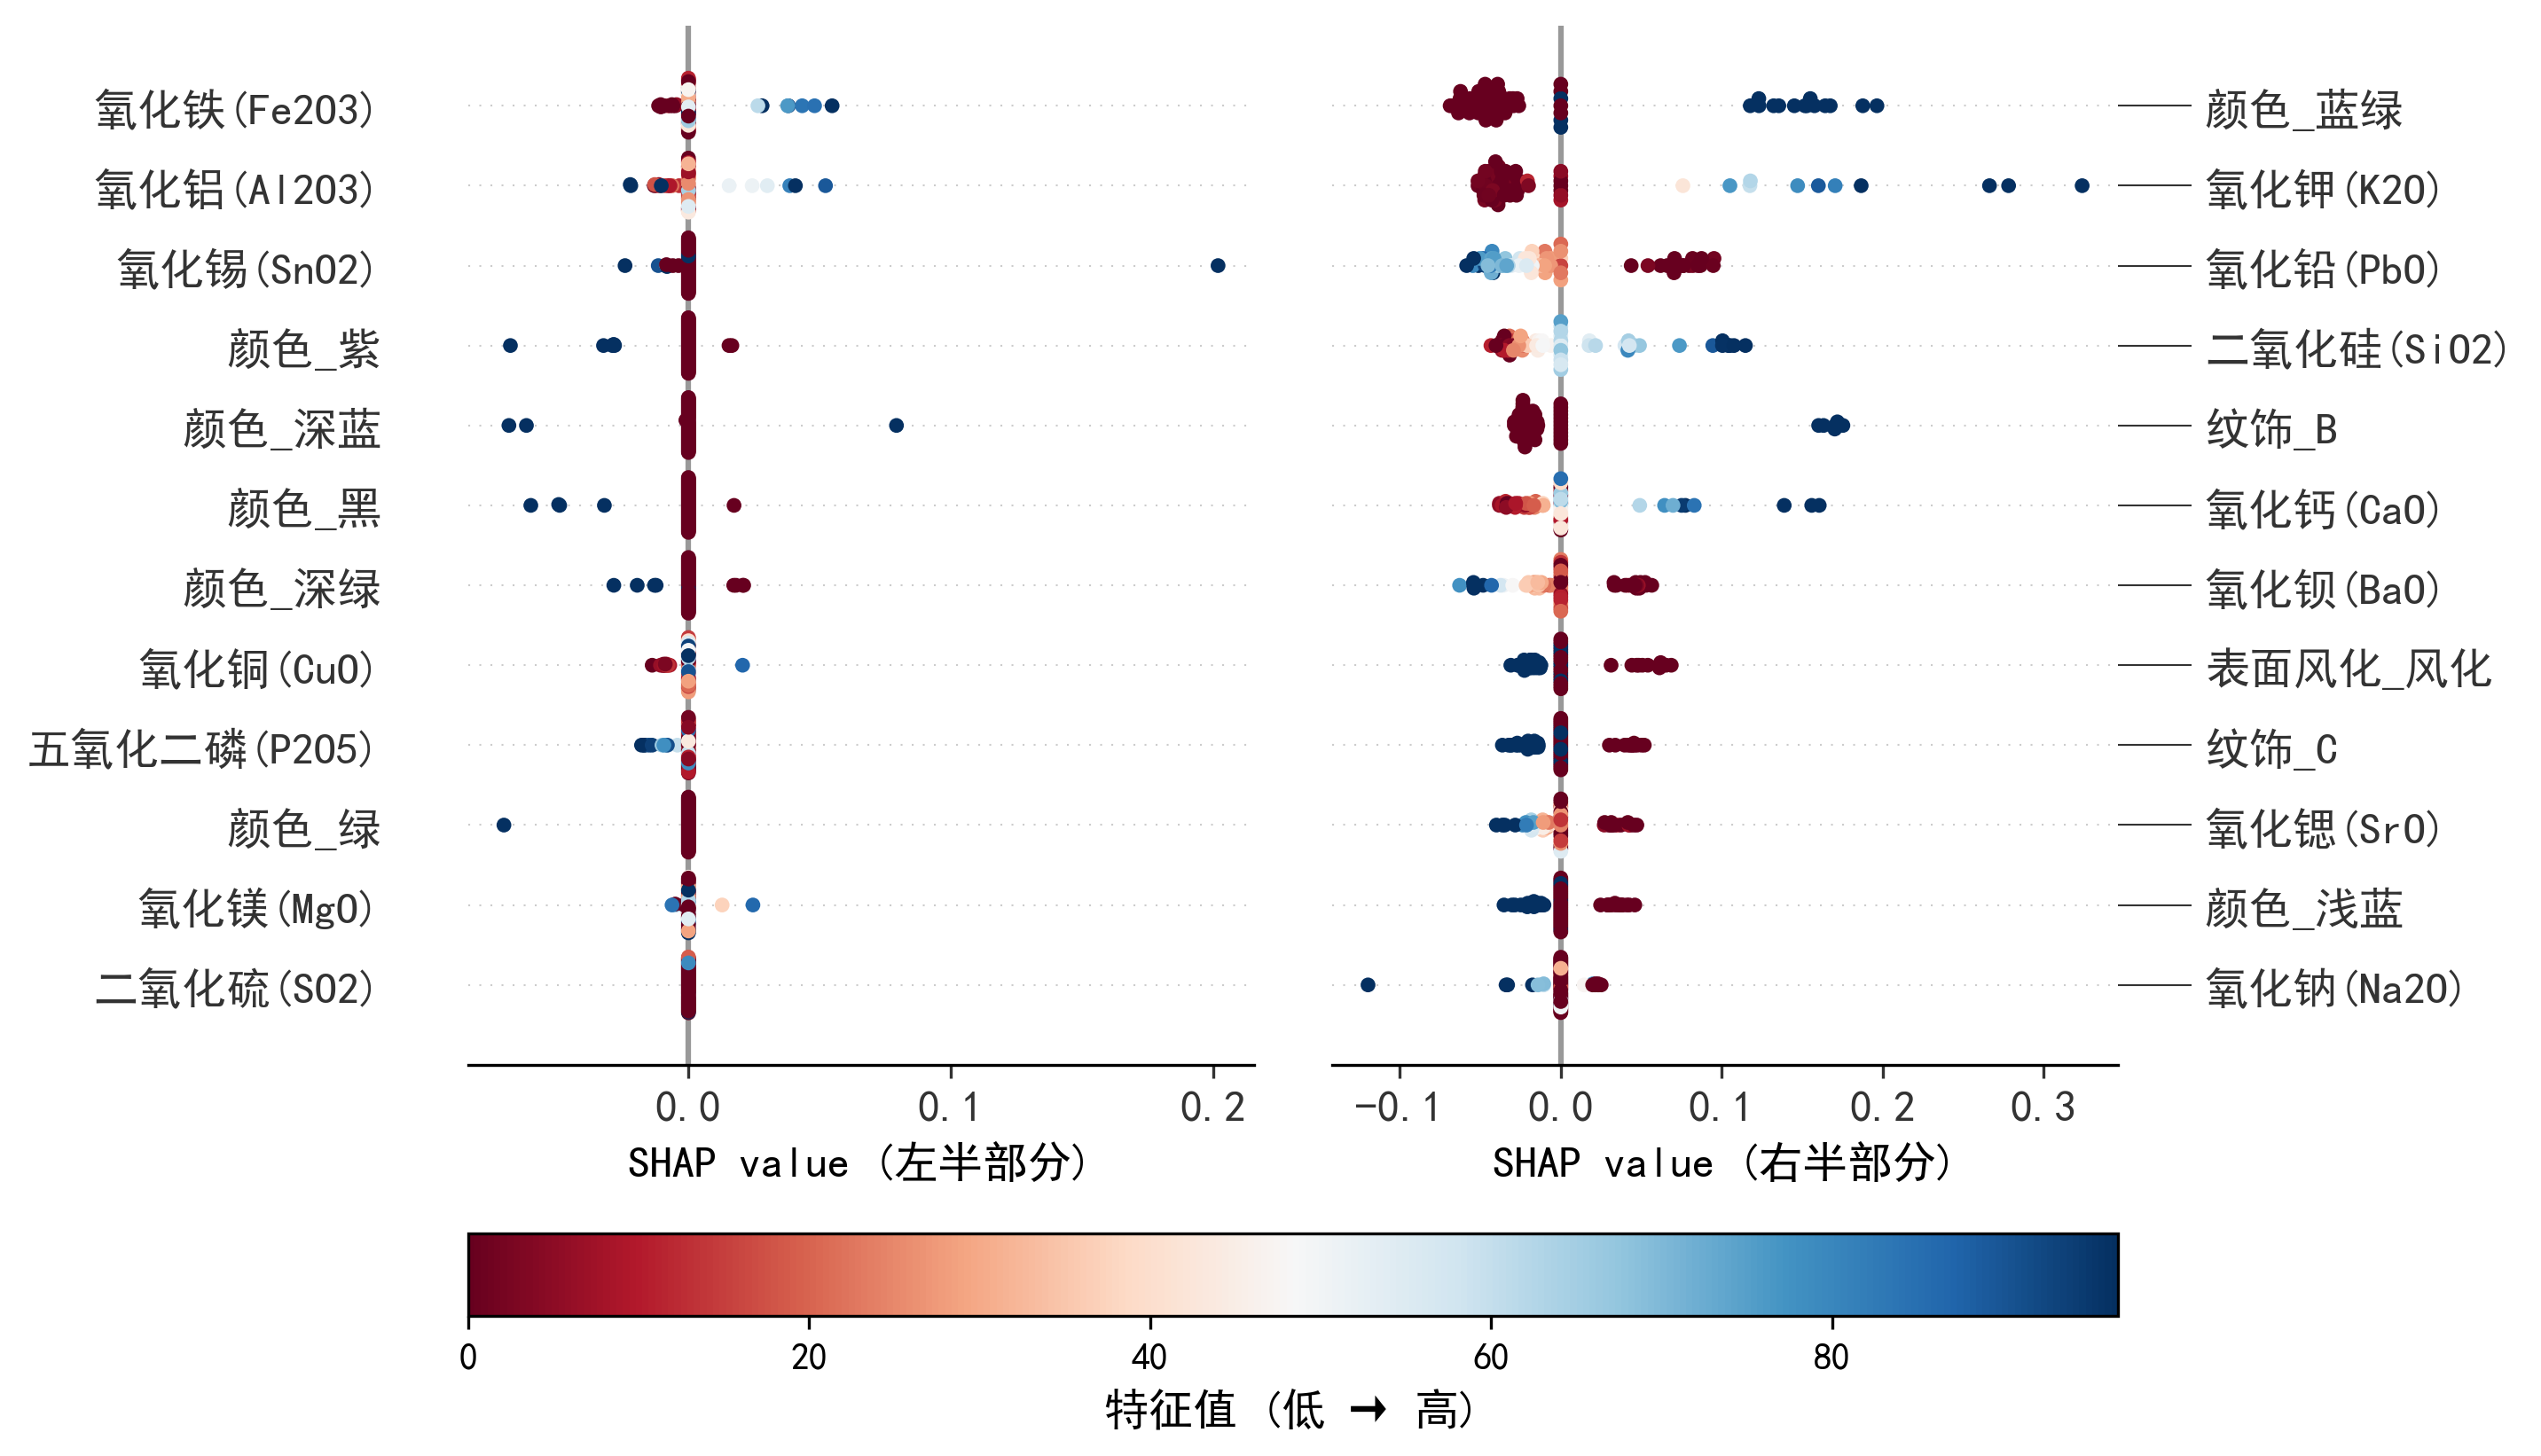
\includegraphics[width=\textwidth]{figs/4问题二/SHAP摘要图_双列_最终版_横置色条.png}
    \caption{非线性支持向量机模型的SHAP全局特征重要性分析}
    \label{fig:shap_summary}
\end{figure}

图\ref{fig:shap_summary}展示了全局特征重要性,纵轴按重要性高低排列特征,横轴是SHAP值,点的颜色代表该特征原始值的大小。该图再次确认$PbO$与$K_2O$是最重要的特征,并且提供了更丰富的细节,高含量的$PbO$红点总是对应着强烈的负向SHAP值,而高含量的$K_2O$红点则总是对应着强烈的正向SHAP值。

\subsection{各类别内部的亚类划分}

亚类划分的目标是探索同一类别文物之间是否存在基于化学成分的更细微群组。因此,分析的最小单元必须是文物个体,而非单个采样点。我们首先整合数据,对同一未风化文物的多个采样点取化学成分平均值,以消除采样位置带来的随机误差。对于风化文物,则优先选取能代表其风化状态的采样点数据进行平均。若风化文物缺乏此类数据,则采用分级条件均值插补,依据类型、颜色、纹饰的相似性为其估算一个风化后的化学成分。此过程最终生成了一个包含三十四个独立文物,且成分状态一致的数据集。

在进行聚类前,需要筛选出适合用于划分亚类的化学成分。亚类划分旨在寻找类别内部的差异,因此变异系数$CV$成为一个合适的指标。它是一个无量纲的相对离散度量,其定义如下
\begin{equation}
    CV = \frac{\sigma}{\mu}
\end{equation}
其中$\sigma$是标准差,$\mu$是均值。变异系数消除了不同化学成分自身含量均值大小的影响,能更公平地比较各特征的真实变异程度。我们据此为高钾和铅钡玻璃分别筛选出类内变异程度最高的化学成分作为聚类特征。
为确定各类玻璃内部可能存在的亚类数量,我们首先采用探索性的层次聚类方法。该方法无需预设类别数量,通过计算样本间的距离,将化学成分最相似的样本逐级合并,其过程可以通过树状图进行可视化。

\begin{figure}[H]
    \centering
    \begin{minipage}{0.48\textwidth}
        \centering
        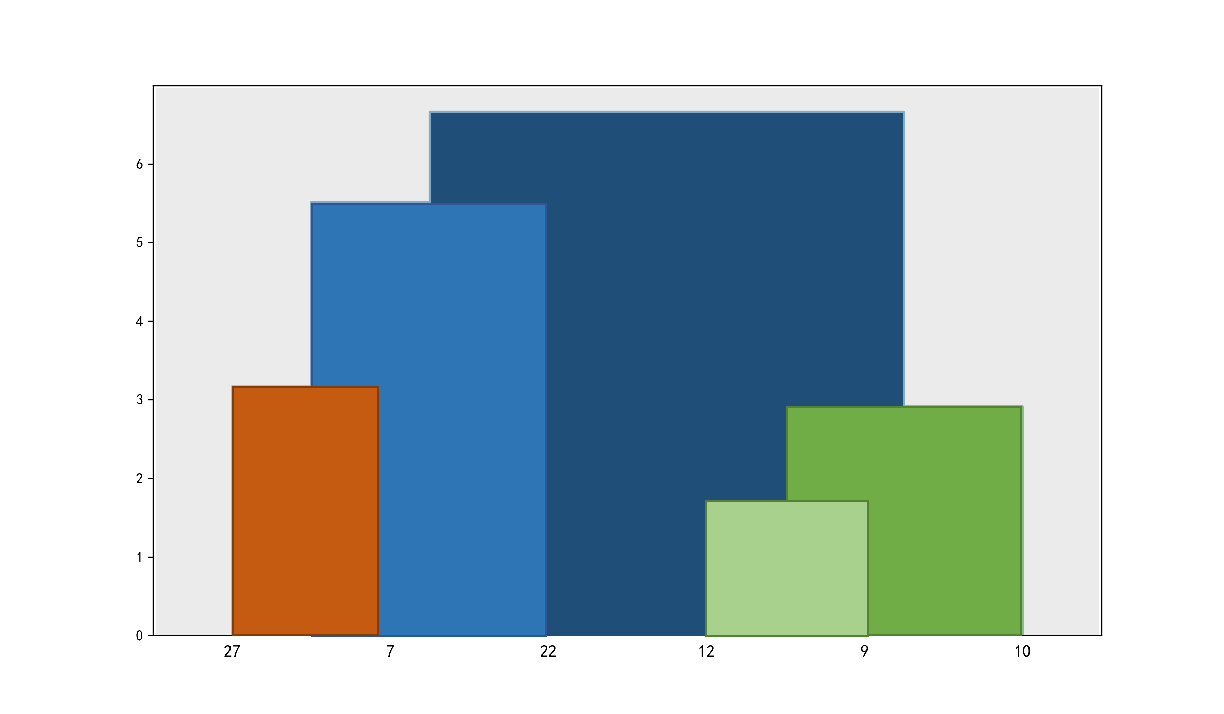
\includegraphics[width=\linewidth]{figs/4问题二/高钾玻璃_层次聚类树状图.png}
        \caption{高钾玻璃层次聚类树状图}
        \label{fig:hclust_k}
    \end{minipage}\hfill
    \begin{minipage}{0.48\textwidth}
        \centering
        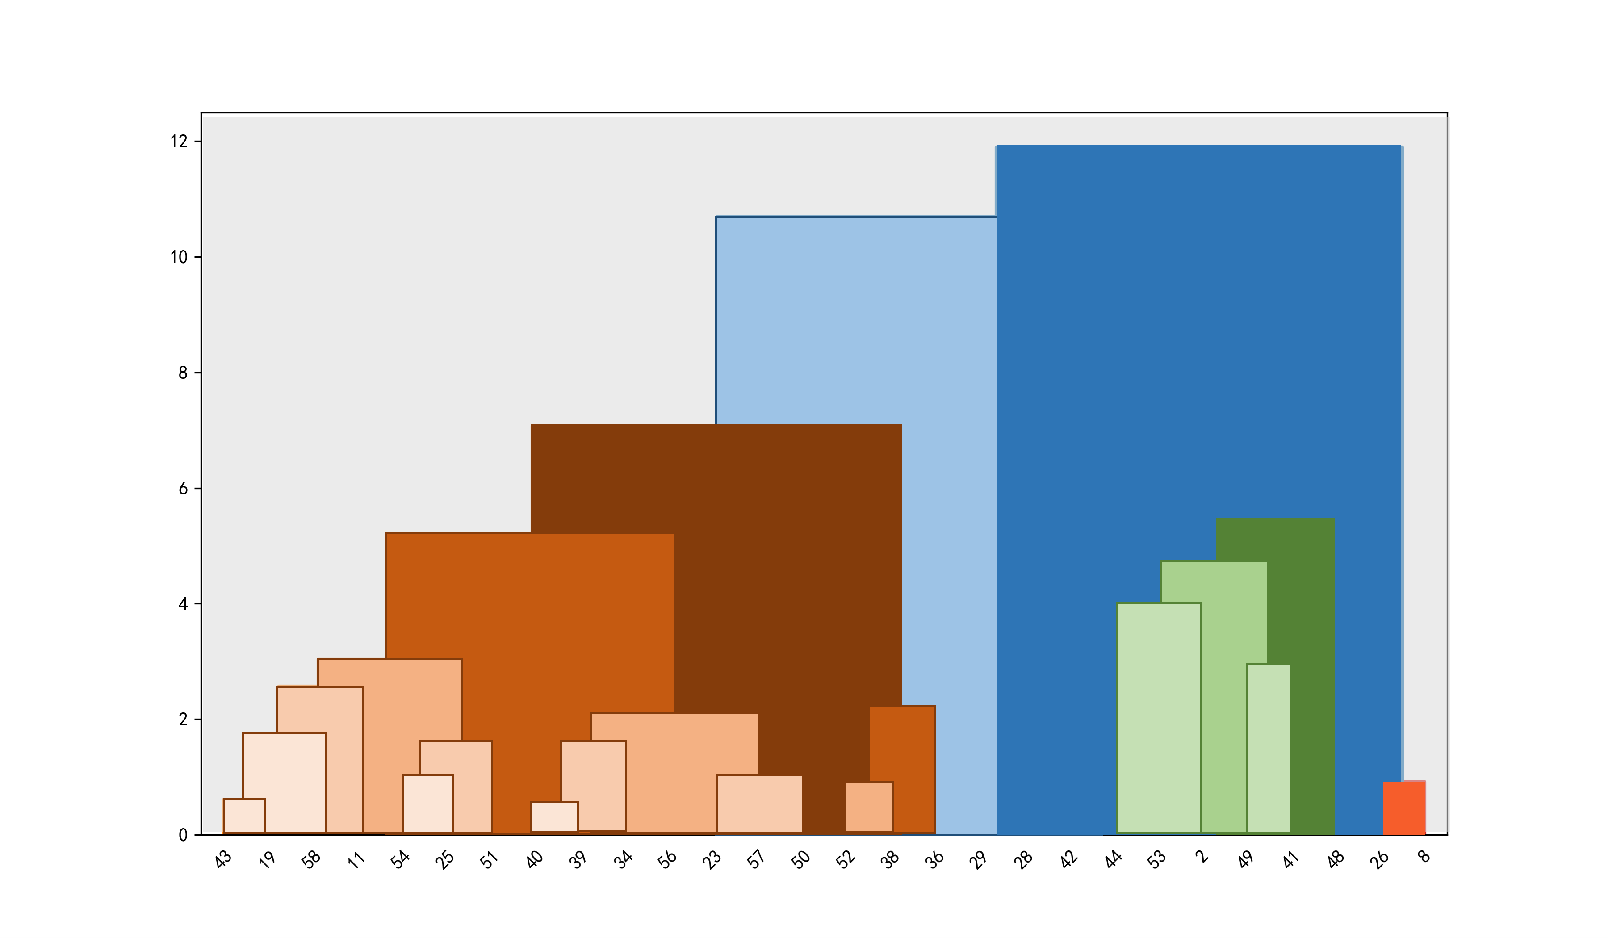
\includegraphics[width=\linewidth]{figs/4问题二/铅钡玻璃_层次聚类树状图.png}
        \caption{铅钡玻璃层次聚类树状图}
        \label{fig:hclust_pb}
    \end{minipage}
\end{figure}

图\ref{fig:hclust_pb}展示的铅钡玻璃树状图呈现出清晰的两分支结构,两个主分支在较高的距离水平上才发生合并,这初步表明铅钡玻璃样本可自然地分为两个大类。相比之下,图\ref{fig:hclust_k}中高钾玻璃的树状图结构更为复杂,呈现出多层次的嵌套聚合模式,表示其内部可能存在更多数量的亚类。

为对亚类数量的选择提供定量依据,我们引入轮廓系数指标。该指标综合评估每个样本与其所属簇的相似度即内聚性,以及与其他簇的差异度即分离度。轮廓系数值越接近一,表示聚类结果的结构越合理。

\begin{figure}[H]
    \centering
    \begin{minipage}{0.48\textwidth}
        \centering
        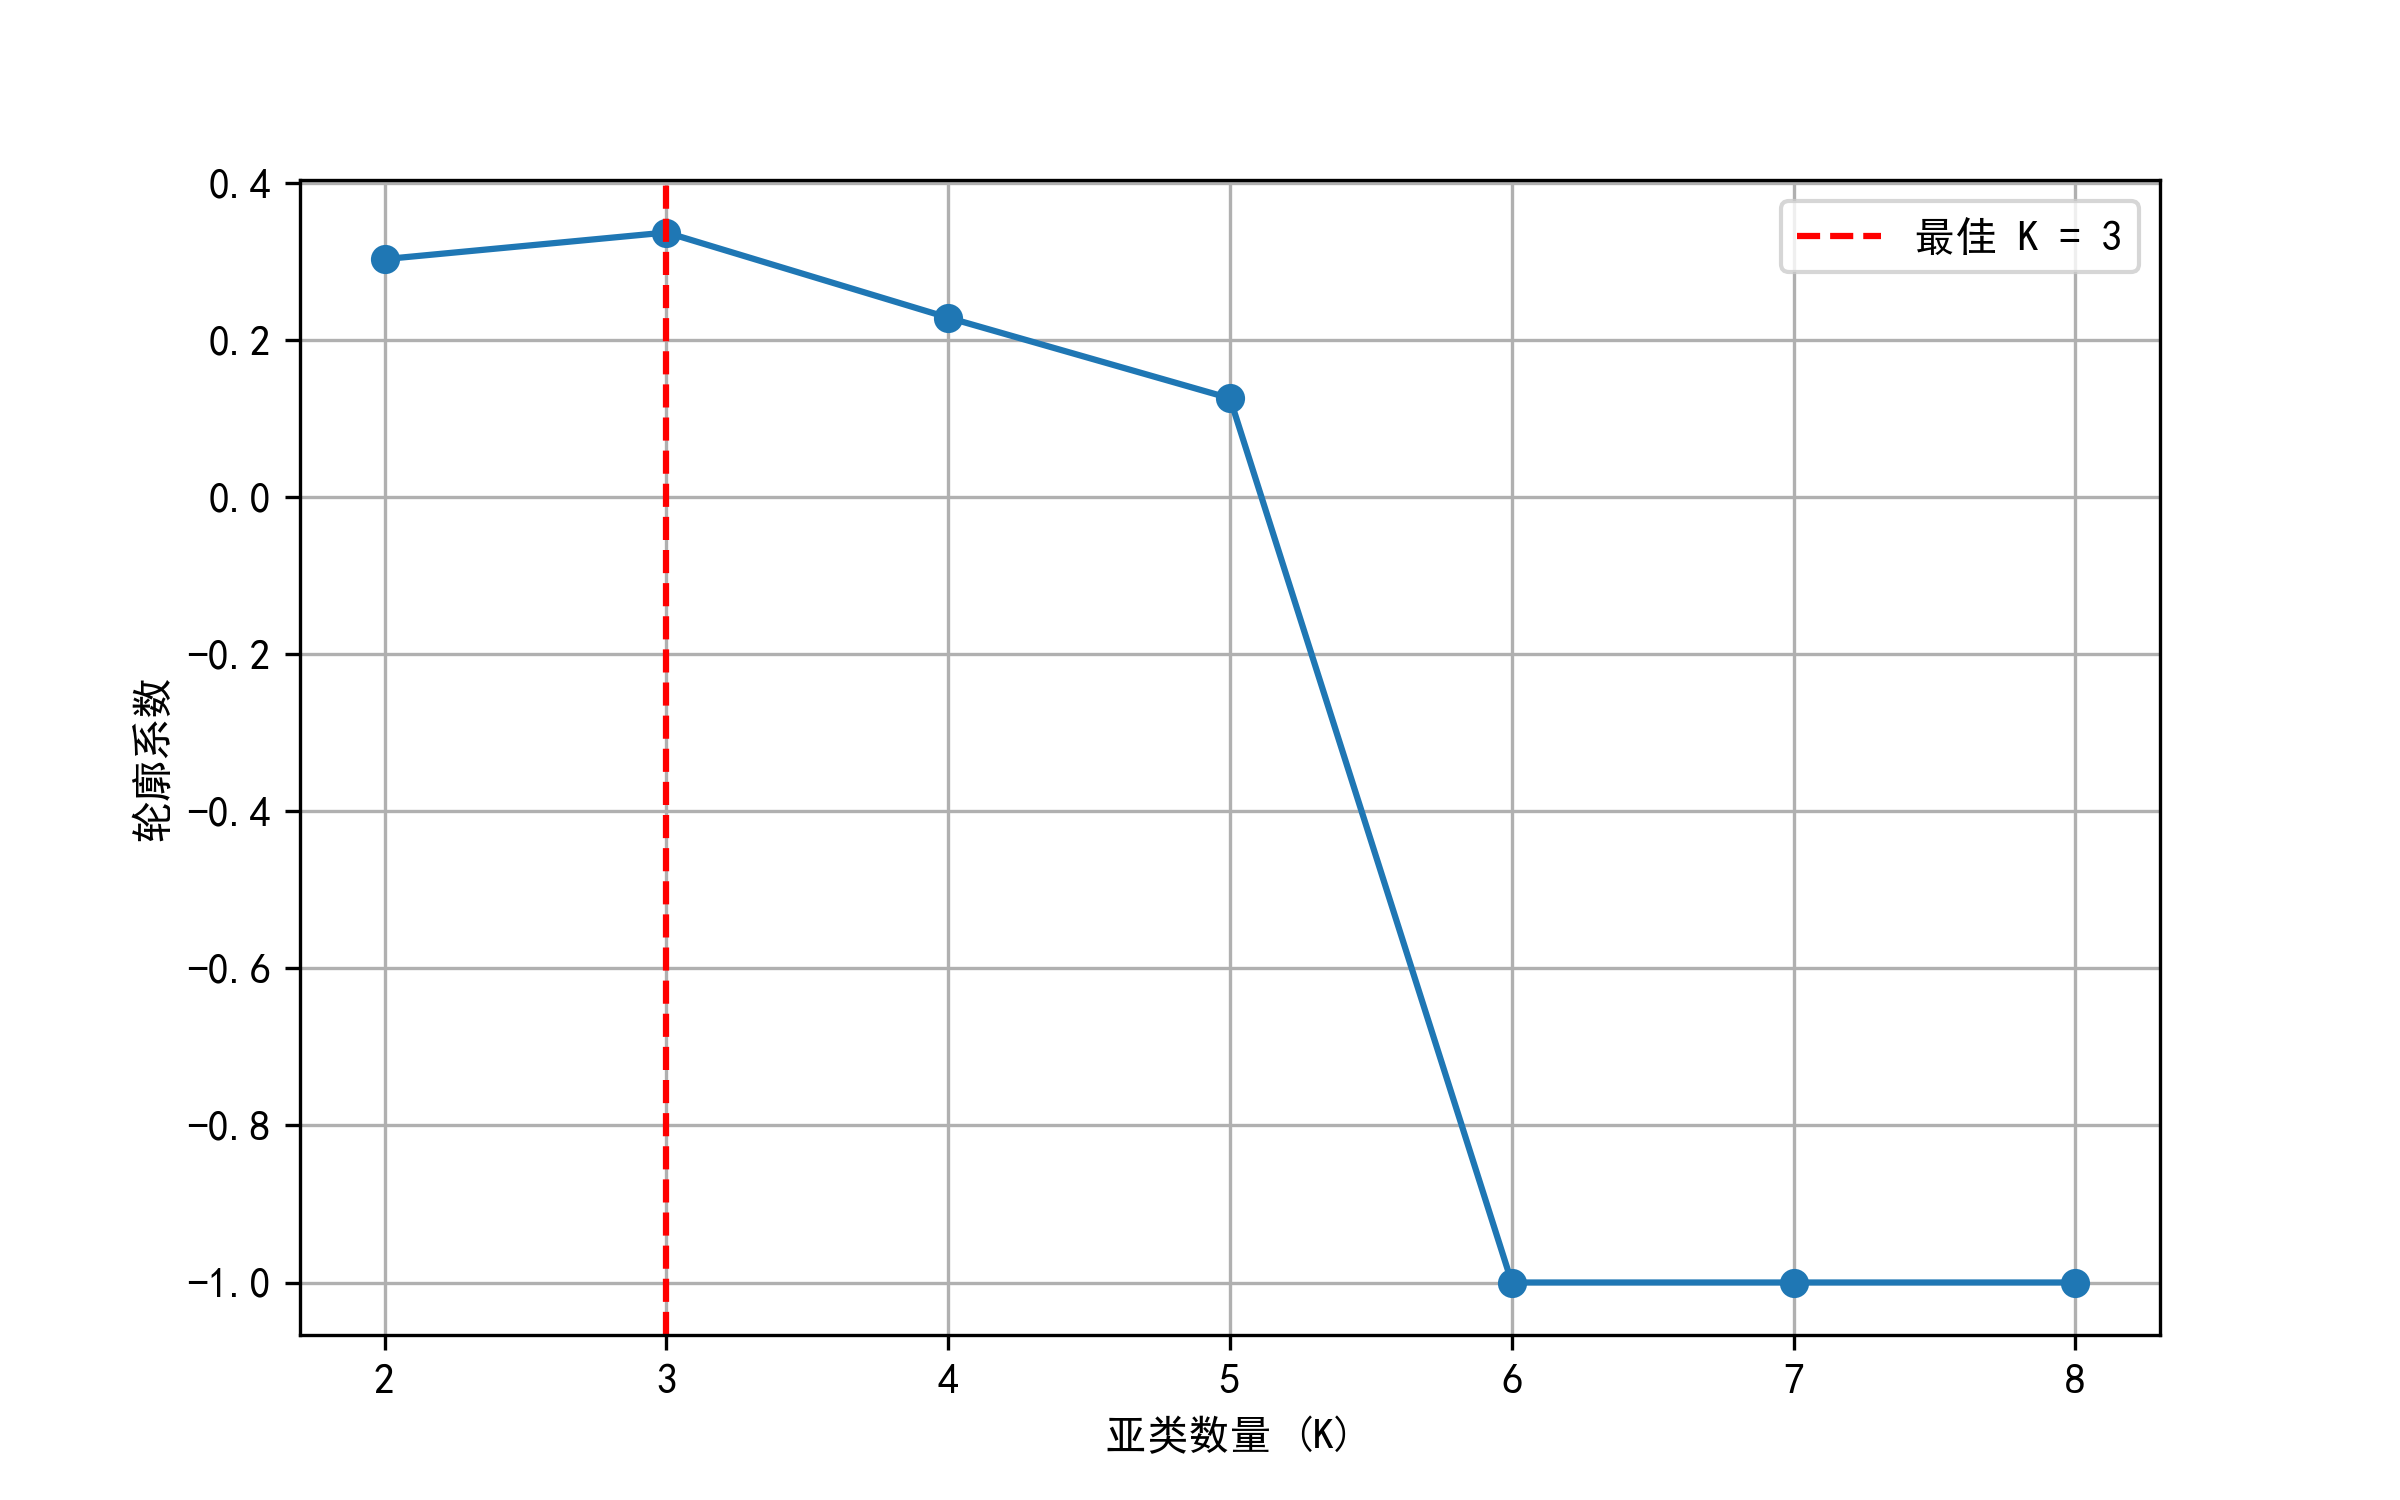
\includegraphics[width=\linewidth]{figs/4问题二/高钾玻璃_最佳K值选择.png}
        \caption{高钾玻璃轮廓系数随K值的变化}
        \label{fig:k_select_k}
    \end{minipage}\hfill
    \begin{minipage}{0.48\textwidth}
        \centering
        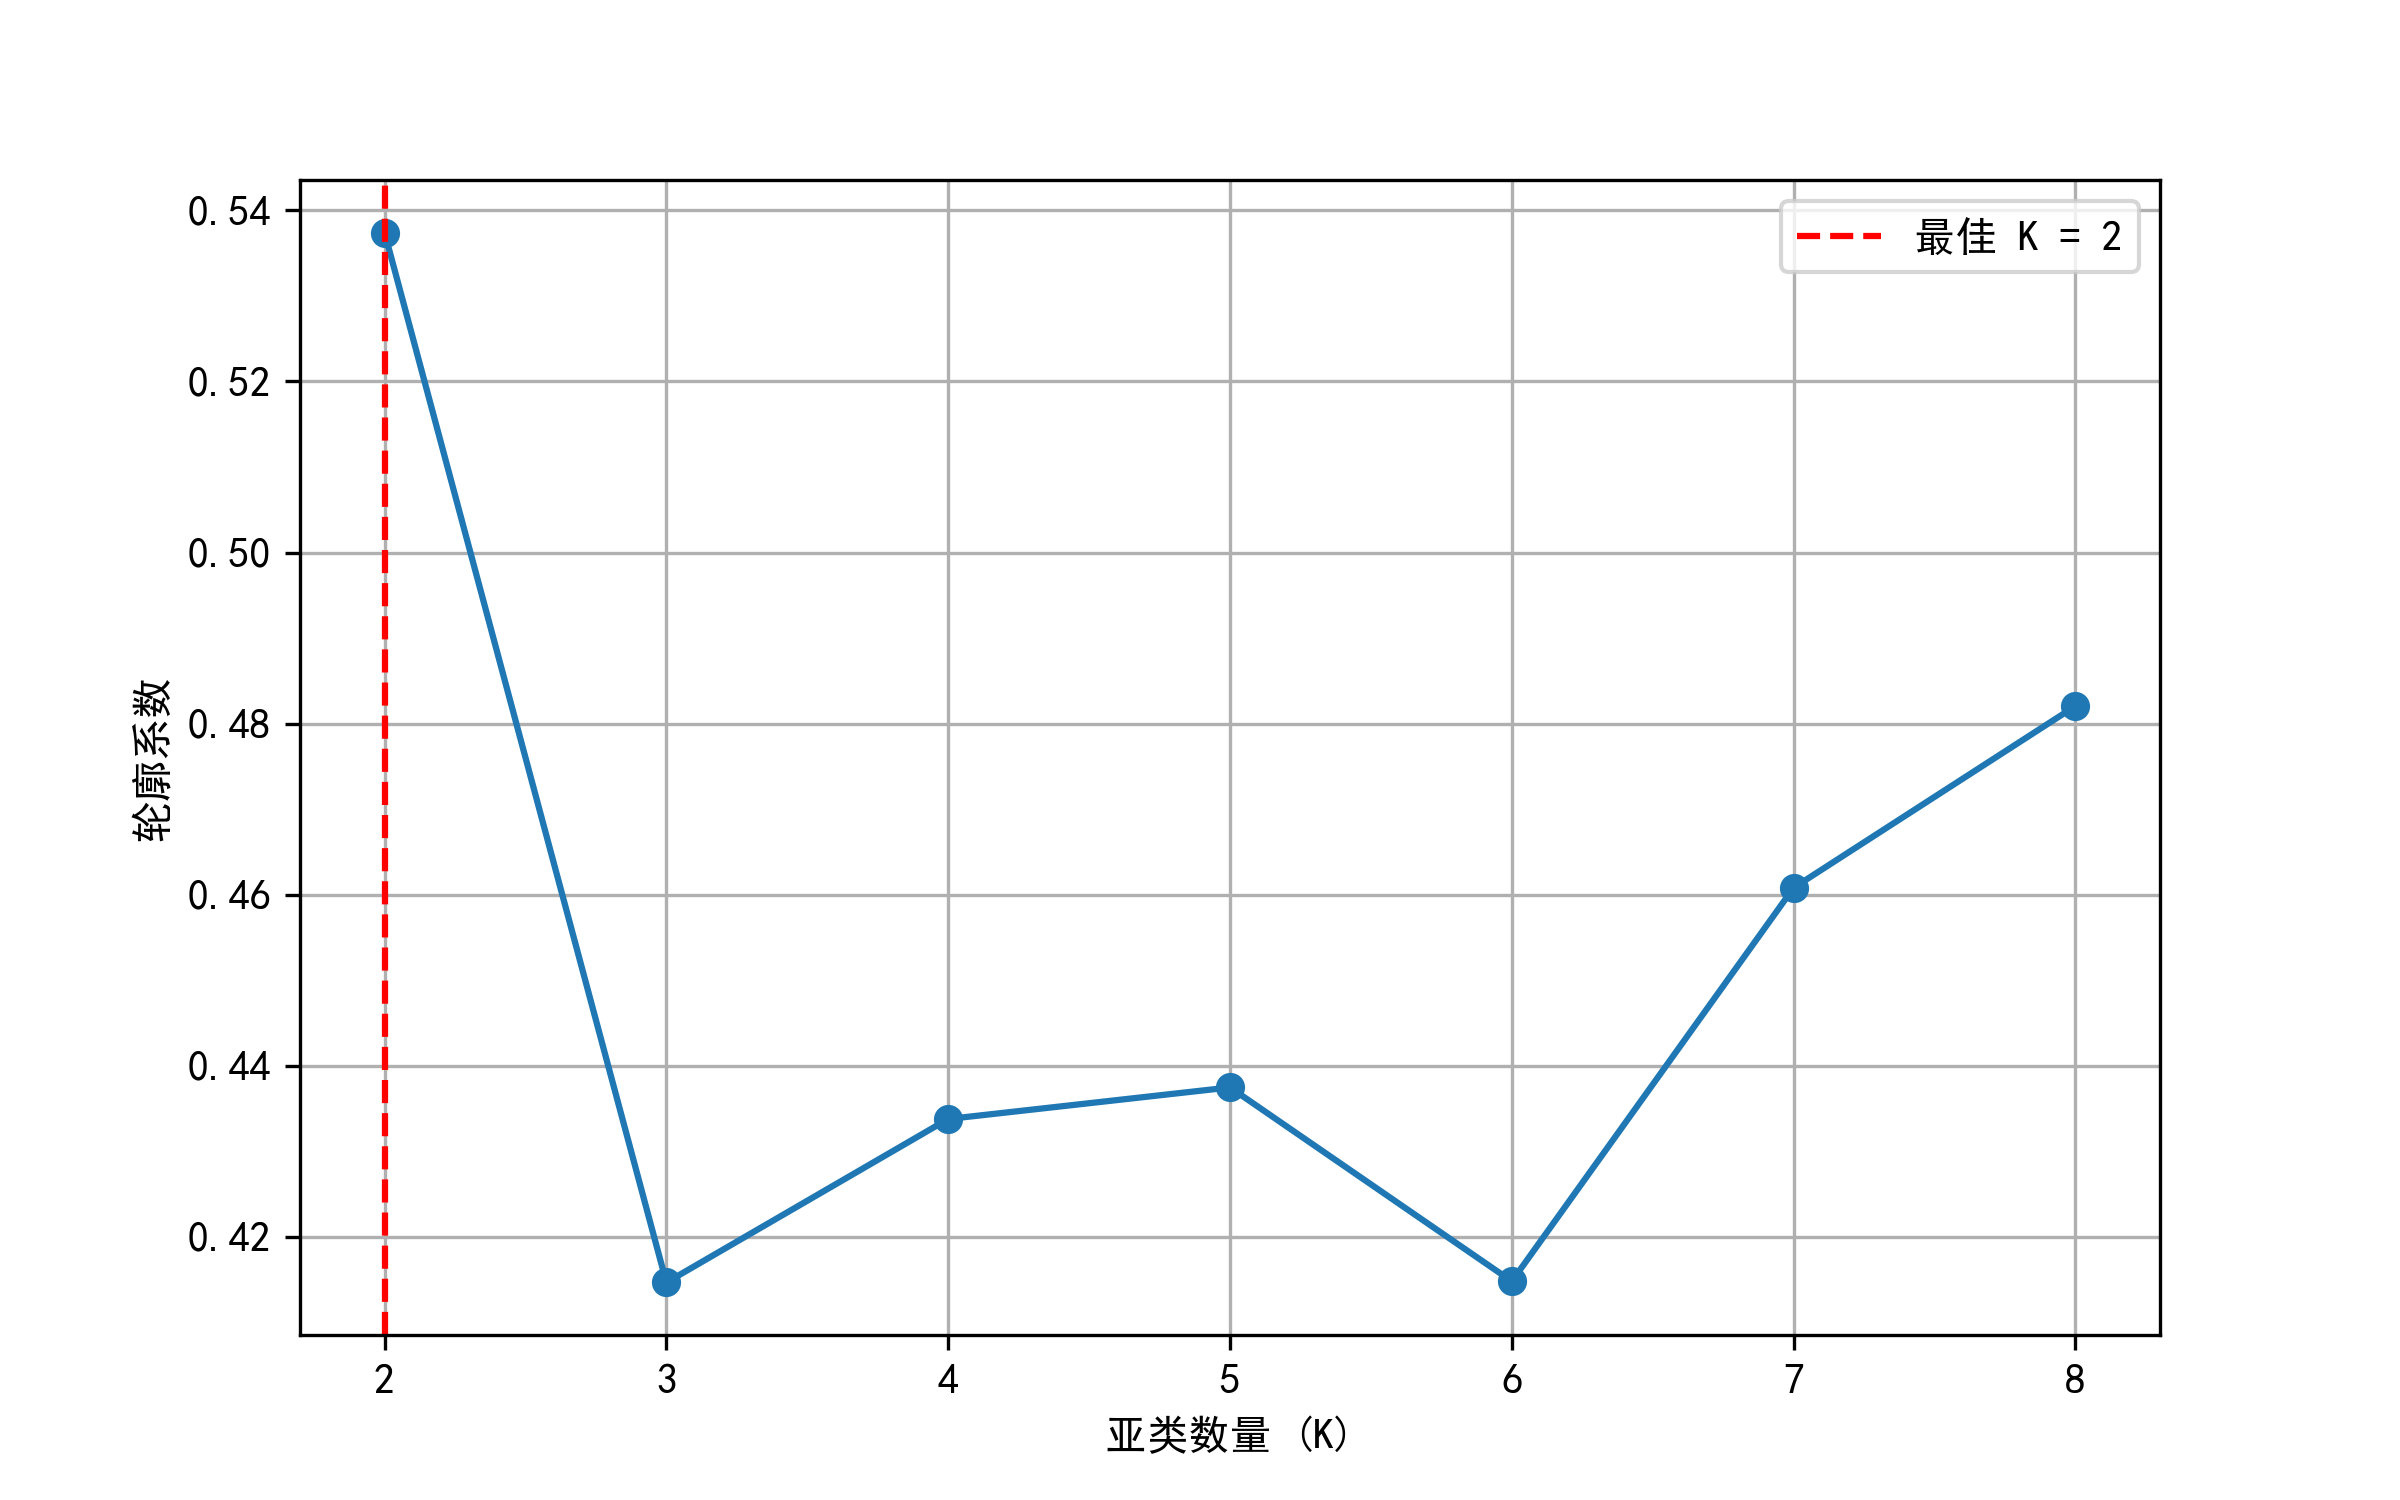
\includegraphics[width=\linewidth]{figs/4问题二/铅钡玻璃_最佳K值选择.png}
        \caption{铅钡玻璃轮廓系数随K值的变化}
        \label{fig:k_select_pb}
    \end{minipage}
\end{figure}

如图\ref{fig:k_select_pb}所示,对于铅钡玻璃,轮廓系数在$K=2$时取得最大值,约为零点四八,当$K$值继续增加时,系数值出现明显下降。对于高钾玻璃,如图\ref{fig:k_select_k}所示,轮廓系数在$K=5$时达到峰值,约为零点五二。综合定性观察与定量计算,我们将铅钡玻璃的亚类数量确定为二,高钾玻璃的亚类数量确定为五。

为验证划分结果的有效性并解读各亚类的化学特征,我们首先利用主成分分析方法将高维的化学成分数据投影到二维平面上。

\begin{figure}[H]
    \centering
    \begin{minipage}{0.48\textwidth}
        \centering
        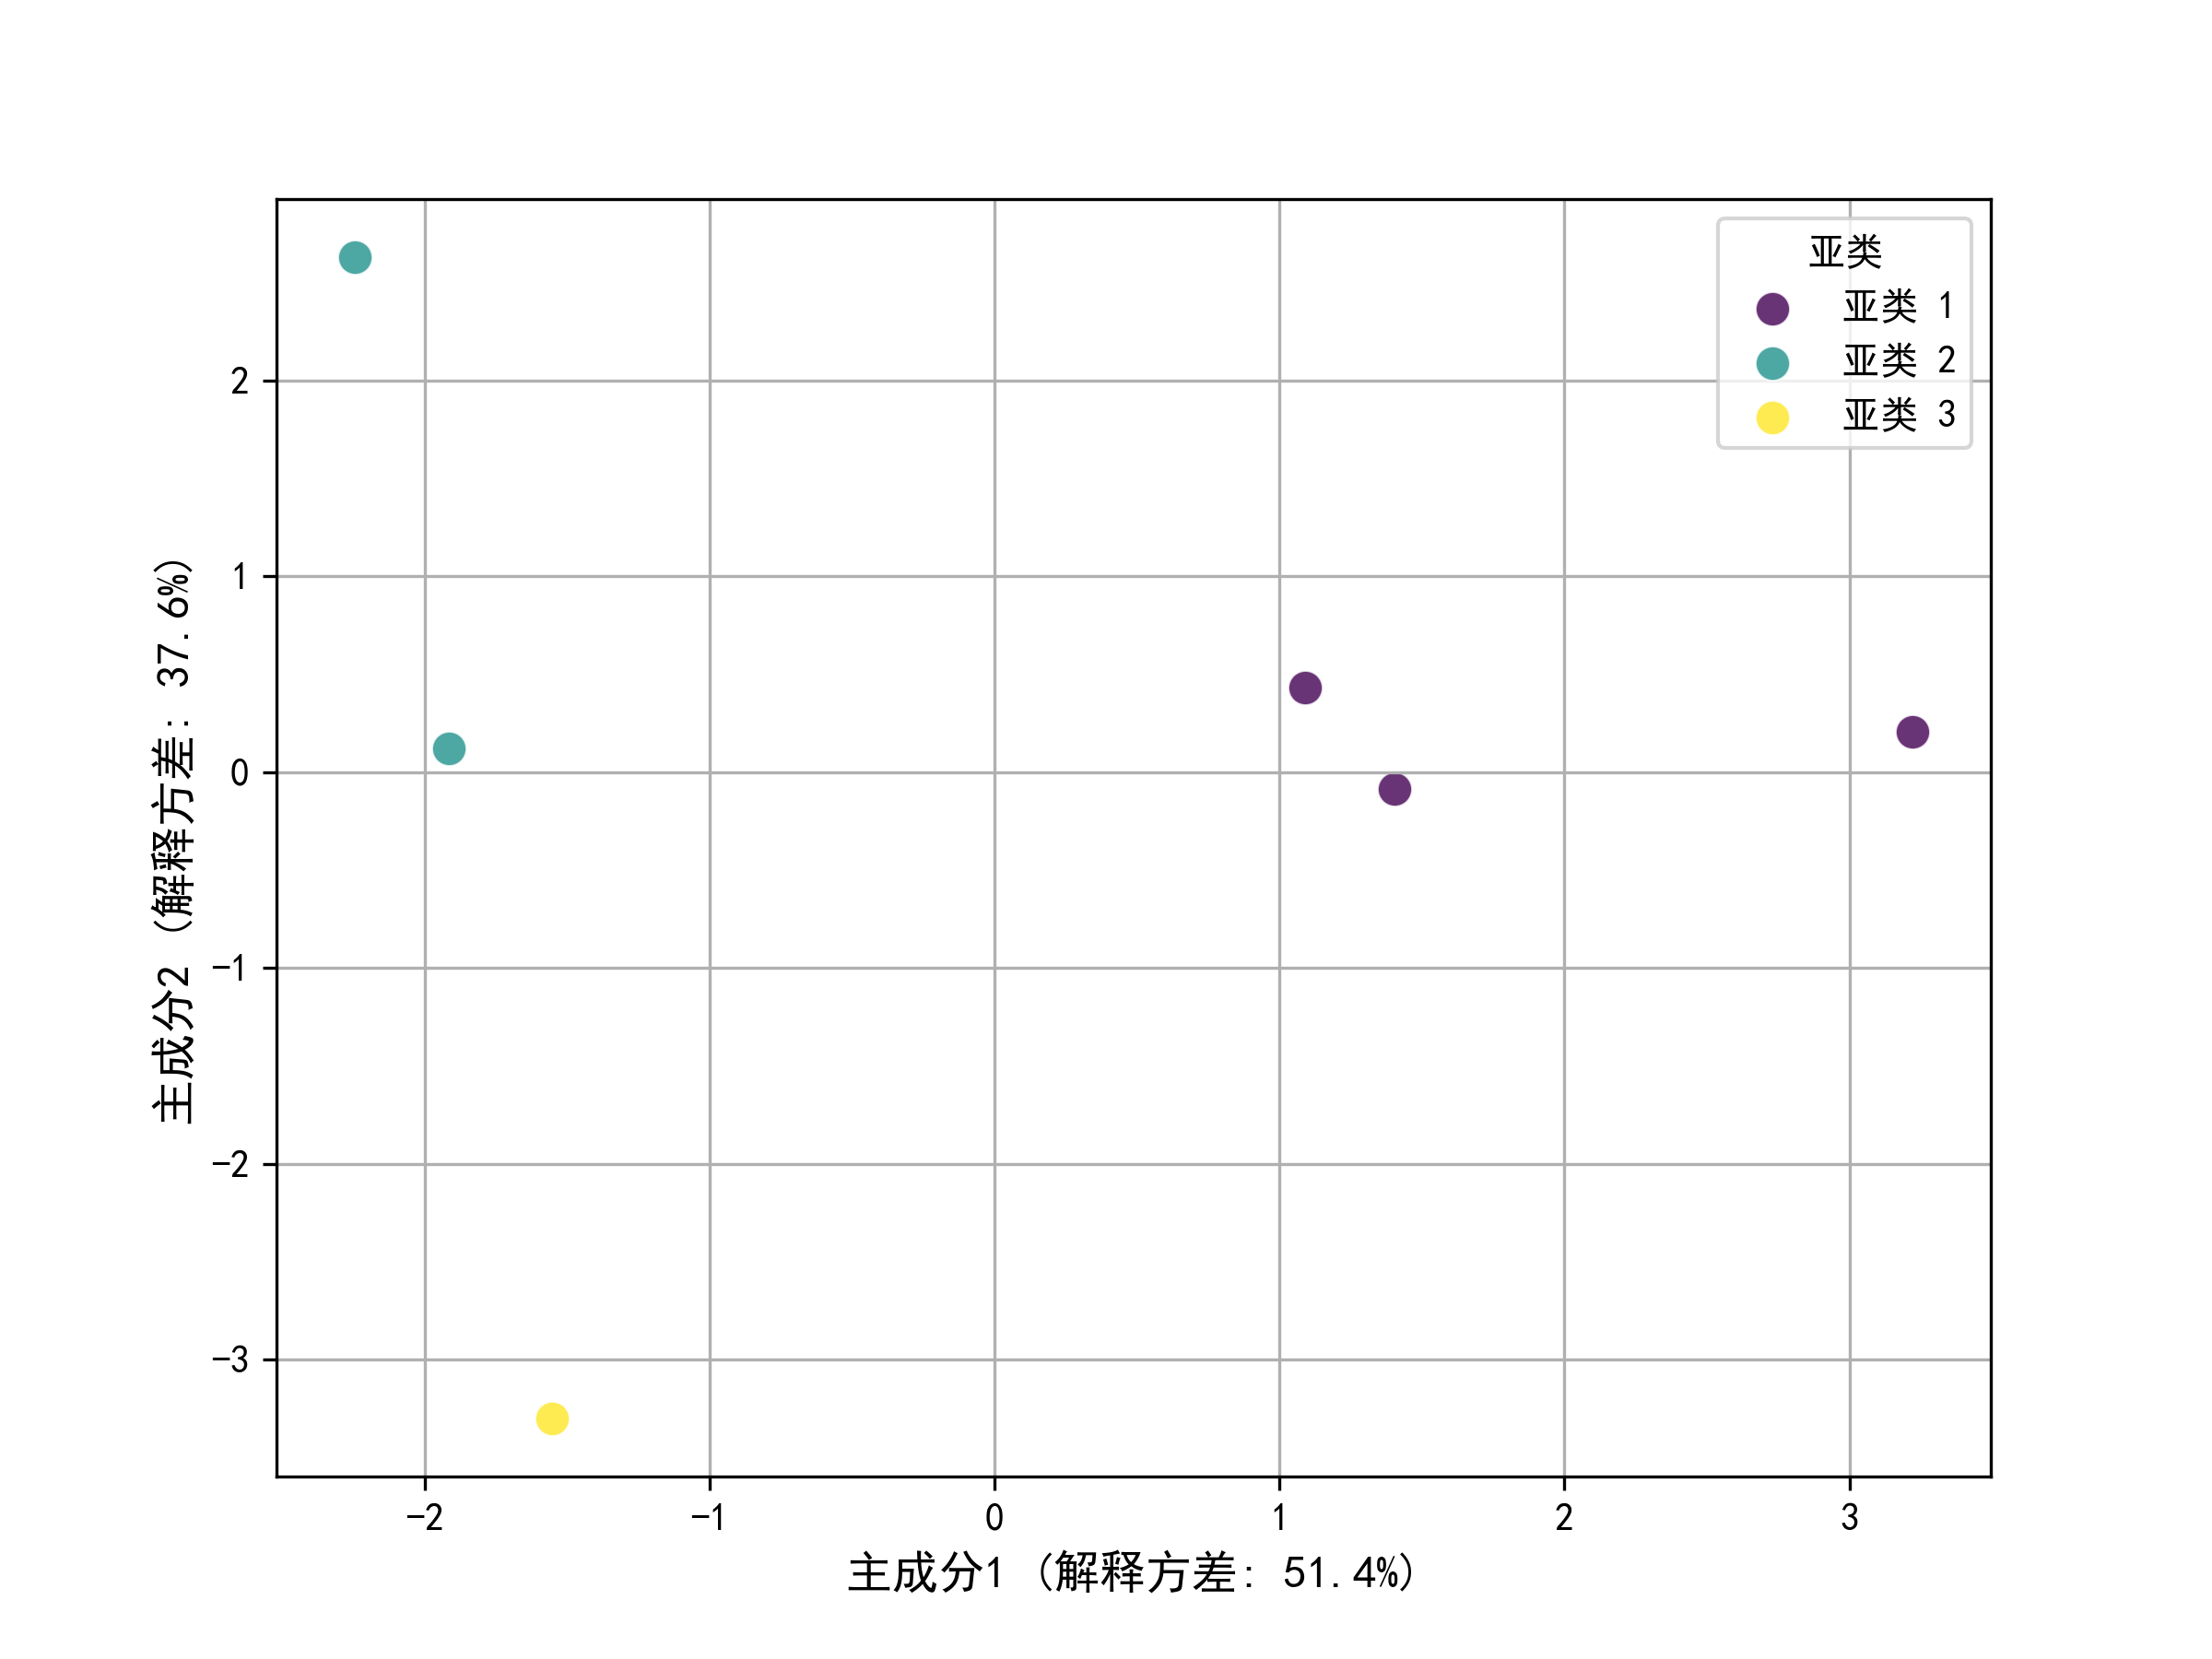
\includegraphics[width=\linewidth]{figs/4问题二/高钾玻璃_亚类PCA图.png}
        \caption{高钾玻璃亚类划分PCA可视化}
        \label{fig:pca_k}
    \end{minipage}\hfill
    \begin{minipage}{0.48\textwidth}
        \centering
        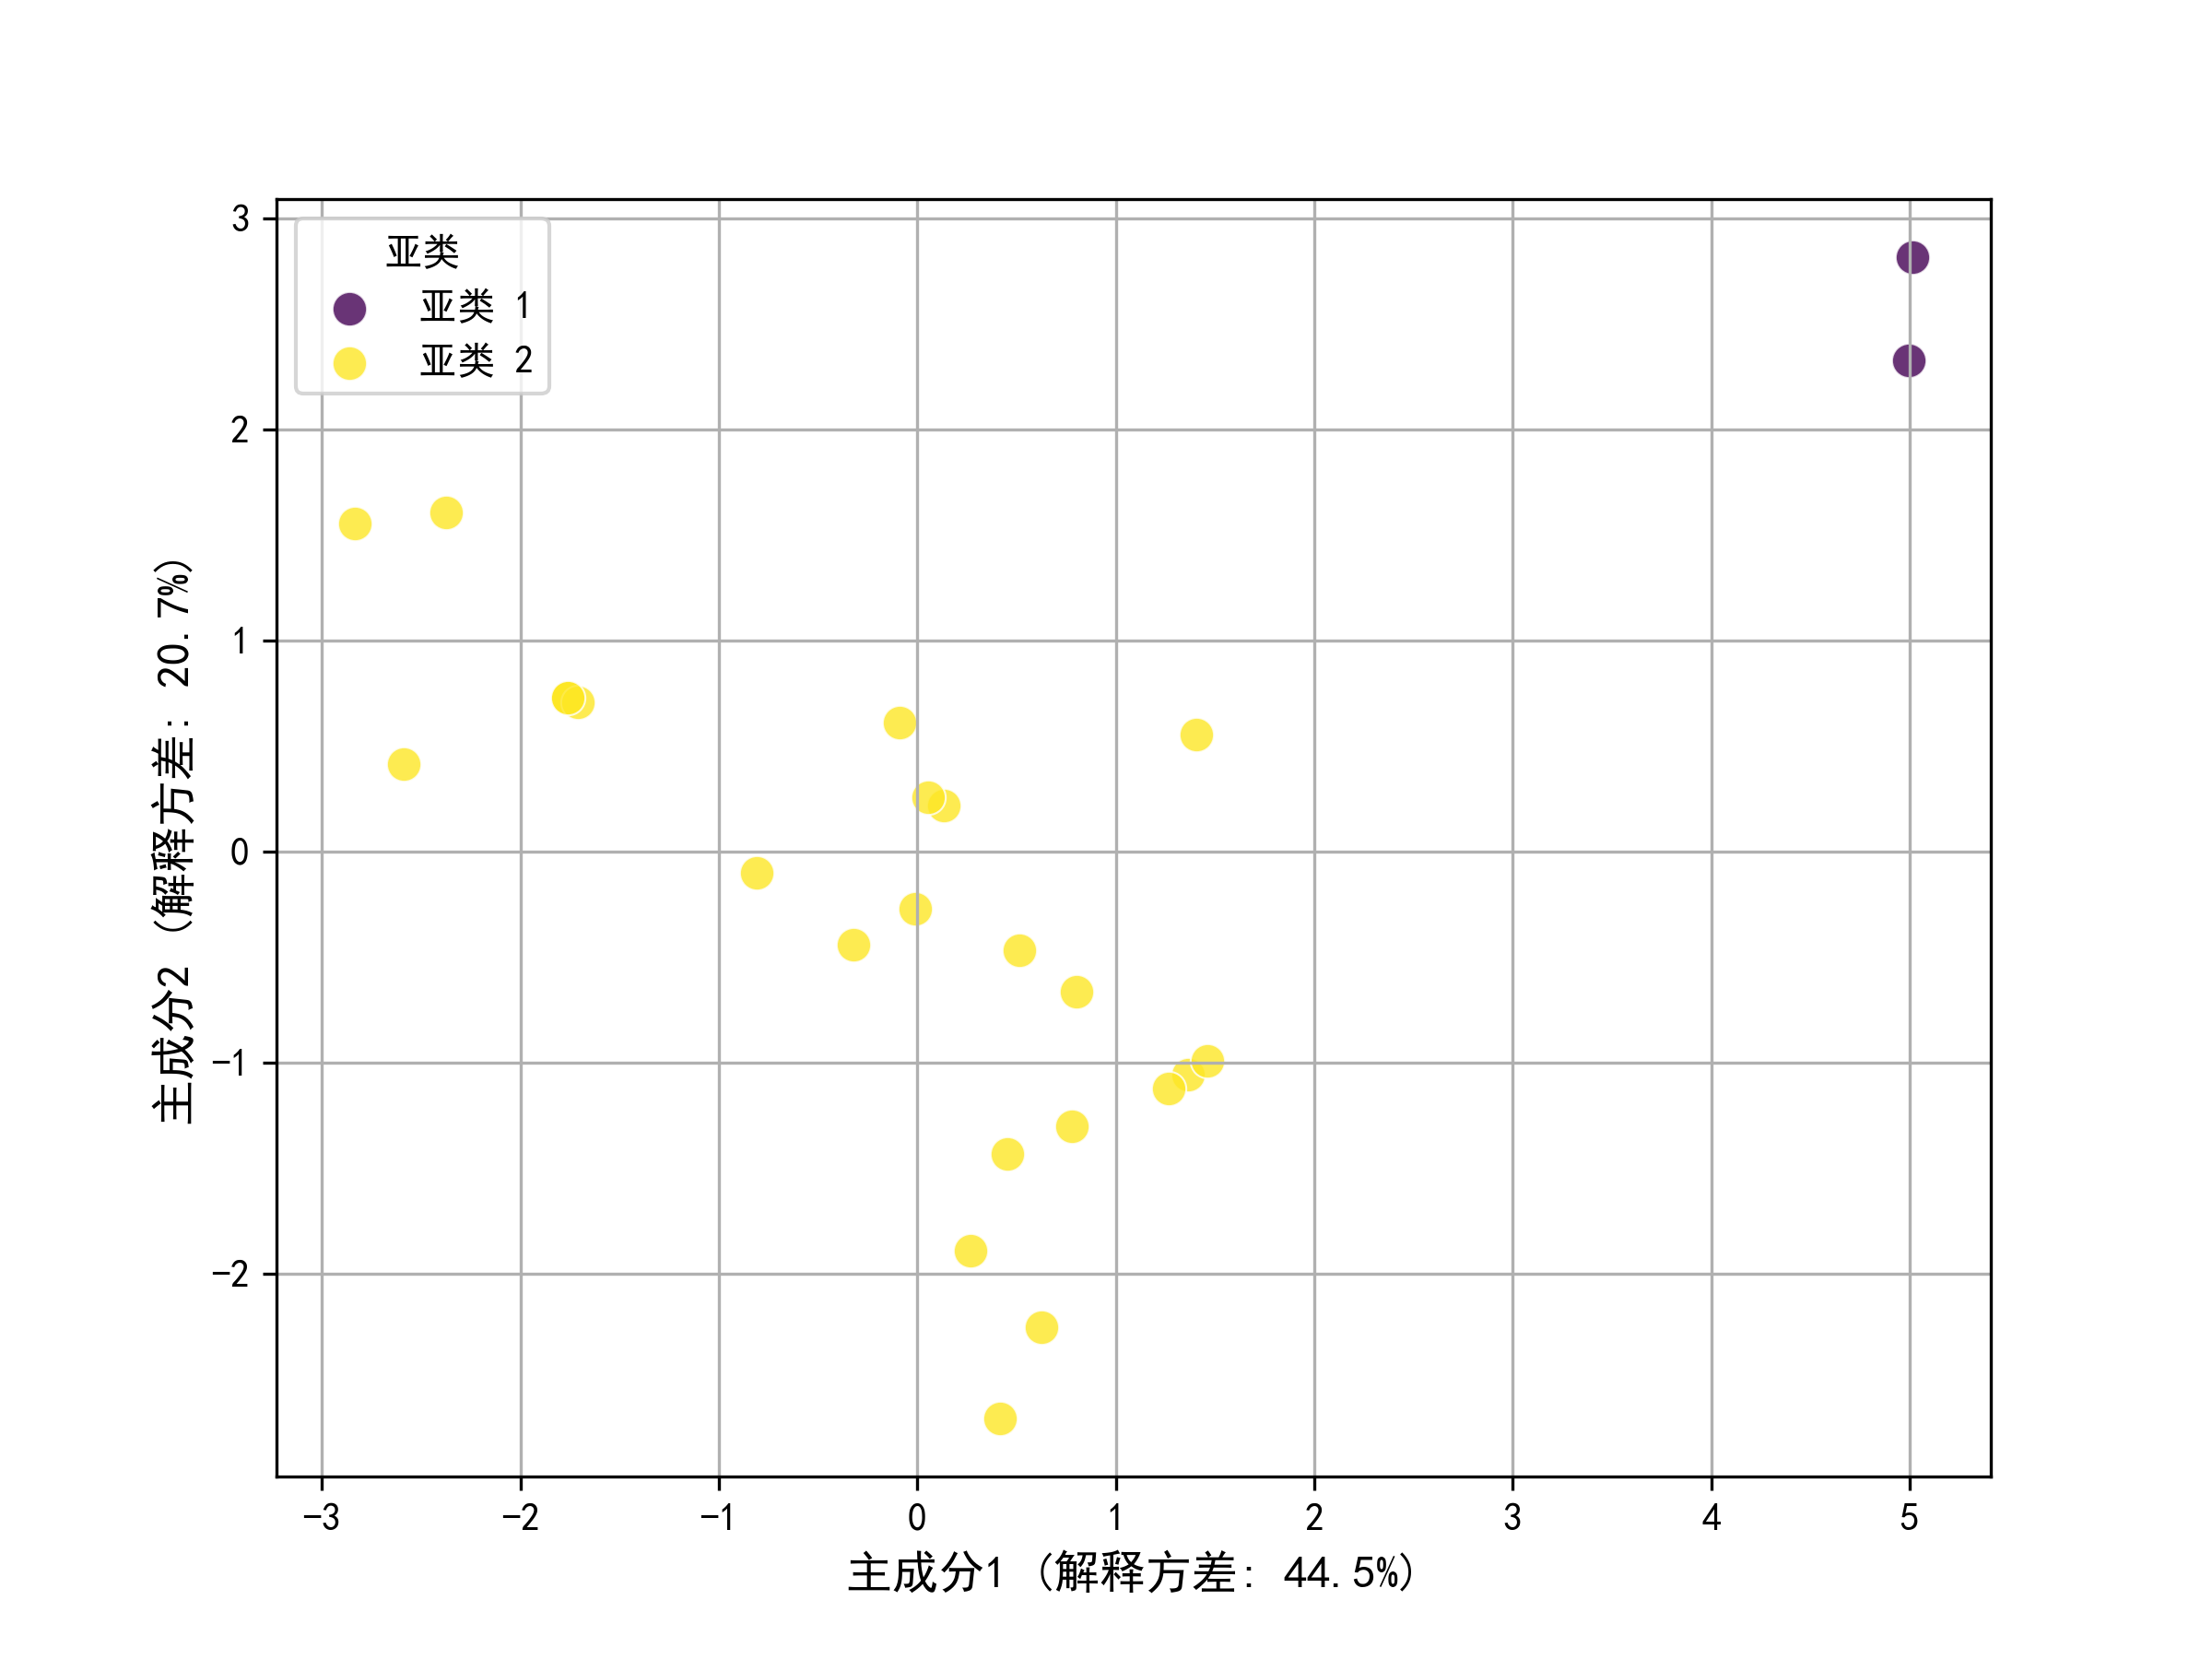
\includegraphics[width=\linewidth]{figs/4问题二/铅钡玻璃_亚类PCA图.png}
        \caption{铅钡玻璃亚类划分PCA可视化}
        \label{fig:pca_pb}
    \end{minipage}
\end{figure}

图\ref{fig:pca_k}与图\ref{fig:pca_pb}的可视化结果显示,不同颜色的点代表不同亚类的样本。铅钡玻璃的两个亚类在第一主成分轴上具有显著的分离。高钾玻璃的五个亚类也在二维空间中占据了相对独立的区域,各亚类内部样本较为集中,而亚类之间存在明显界限。

为进一步阐释每个亚类所代表的化学成分模式,我们绘制了亚类化学特征热力图。

\begin{figure}[H]
    \centering
    \begin{minipage}{0.48\textwidth}
        \centering
        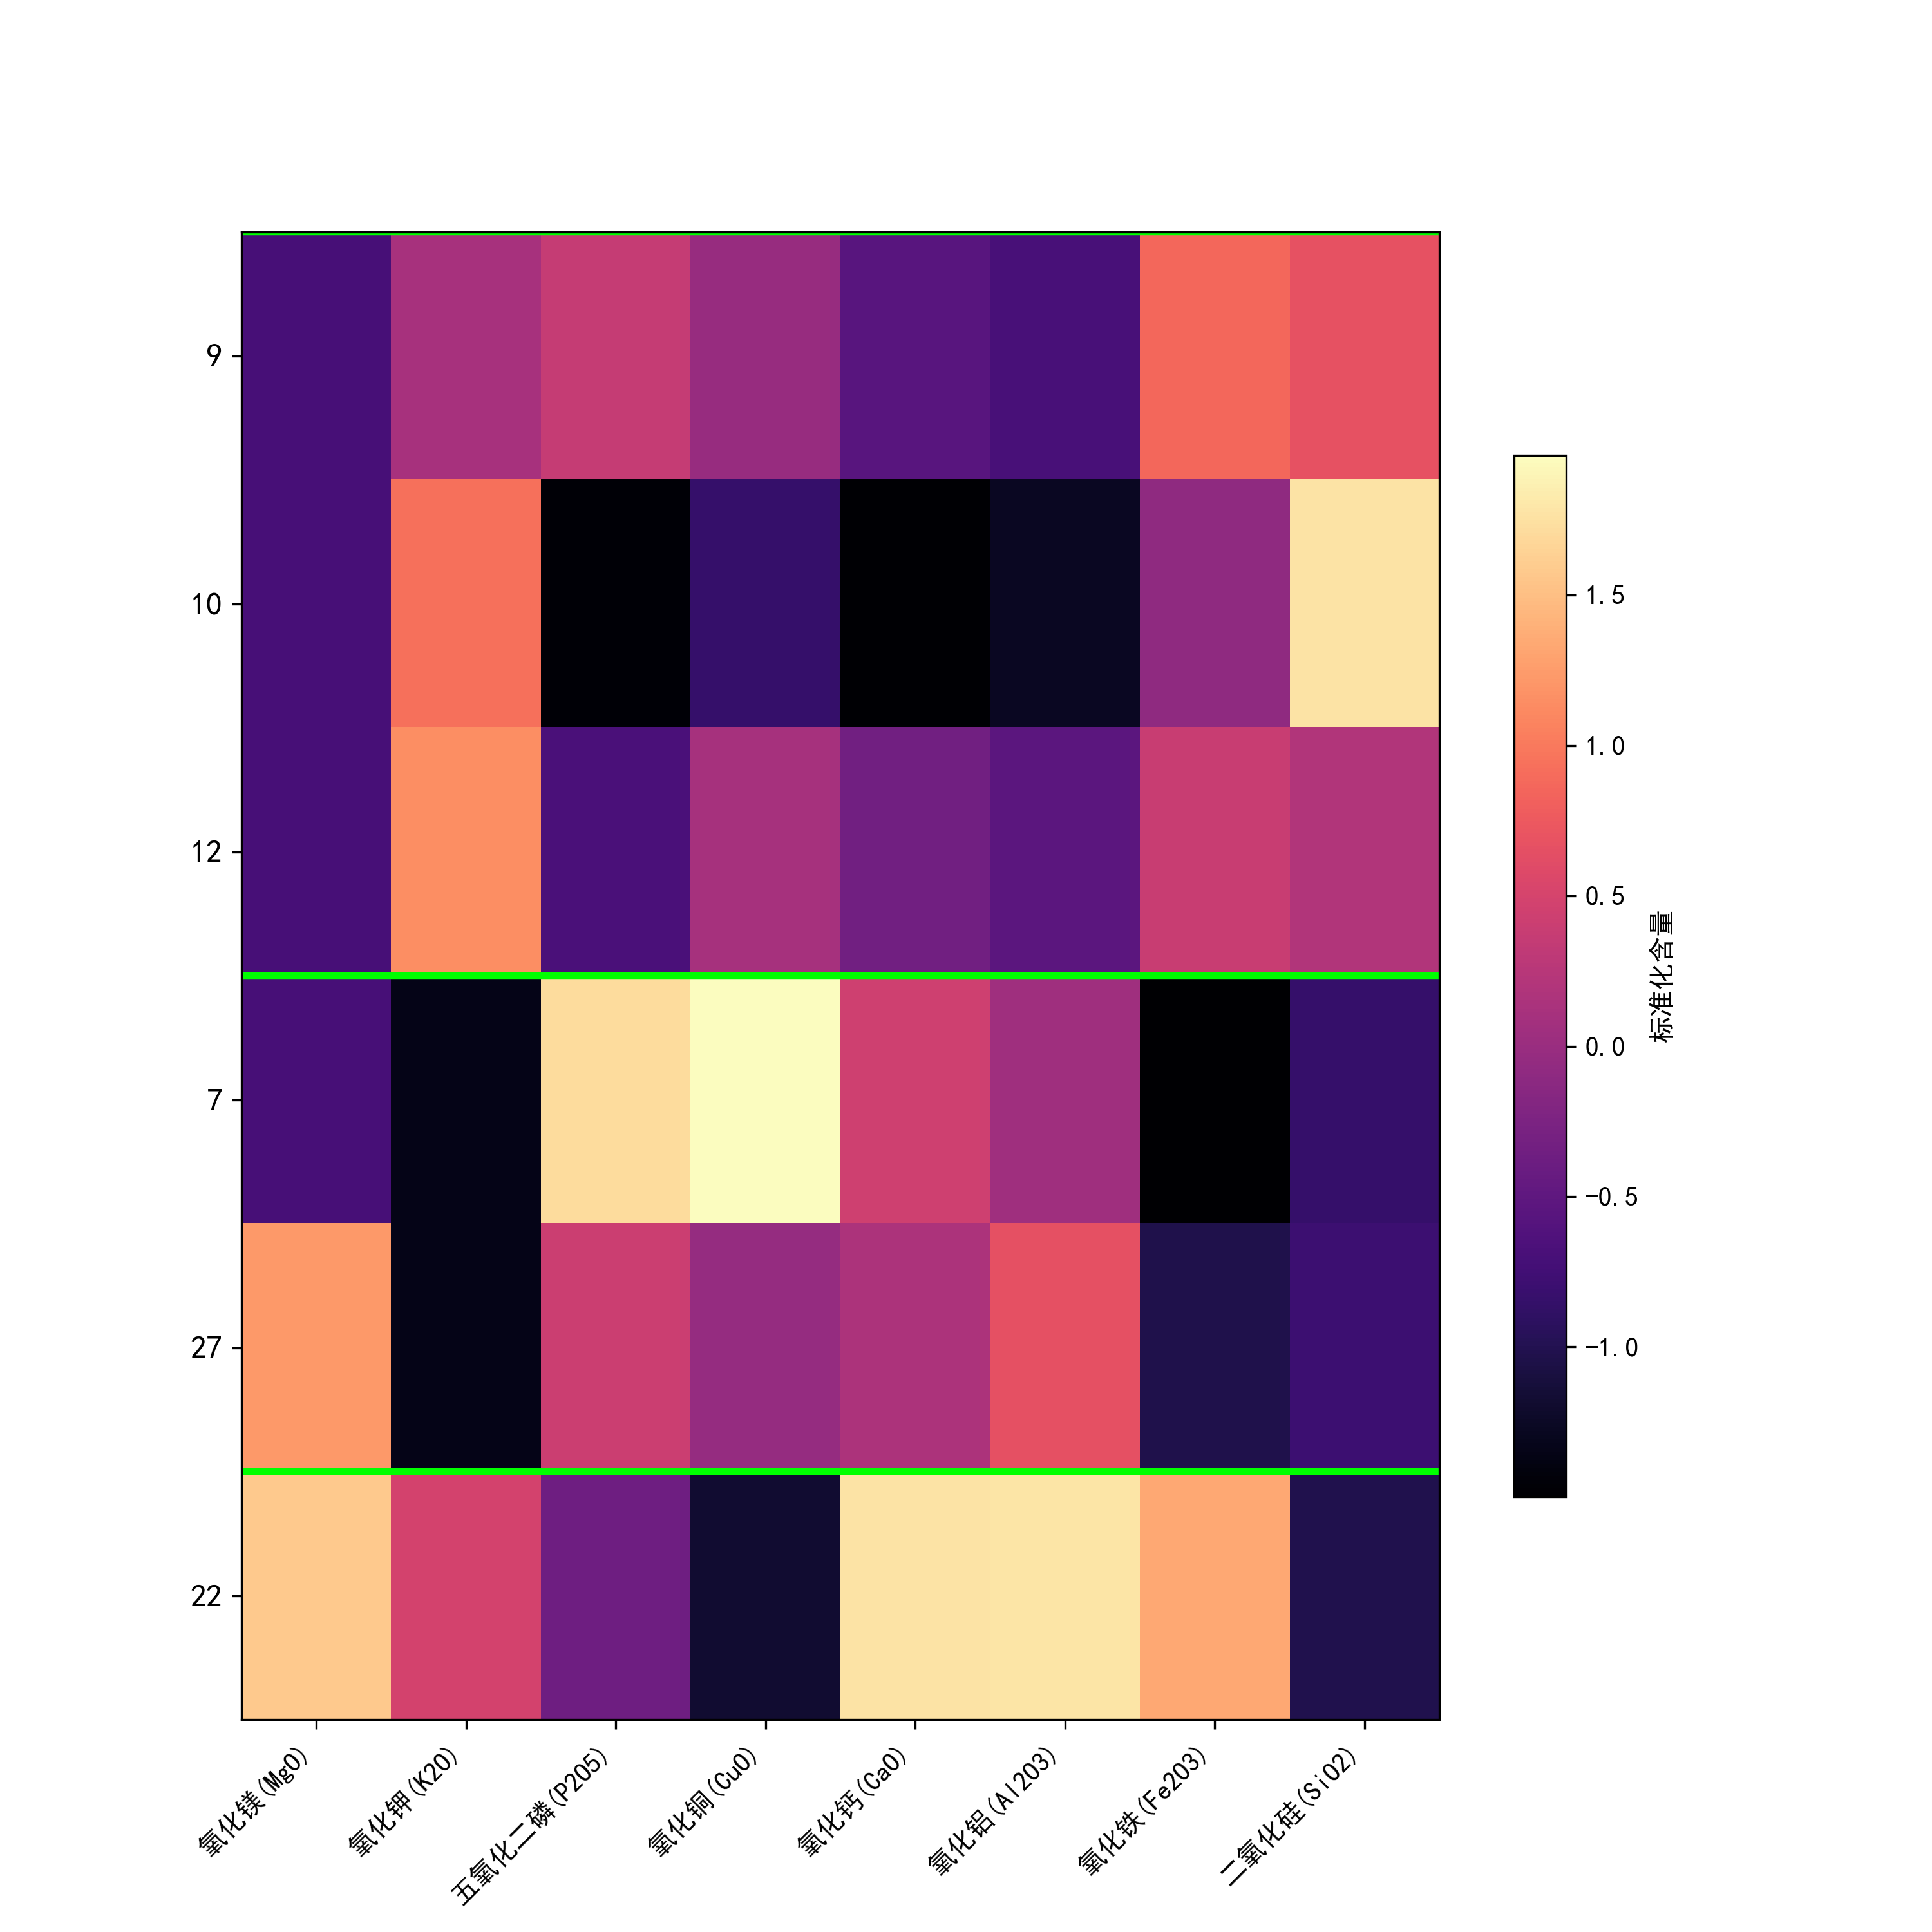
\includegraphics[width=\linewidth]{figs/4问题二/高钾玻璃_亚类热力图_带编号.png}
        \caption{高钾玻璃亚类化学特征热力图}
        \label{fig:heatmap_k}
    \end{minipage}\hfill
    \begin{minipage}{0.48\textwidth}
        \centering
        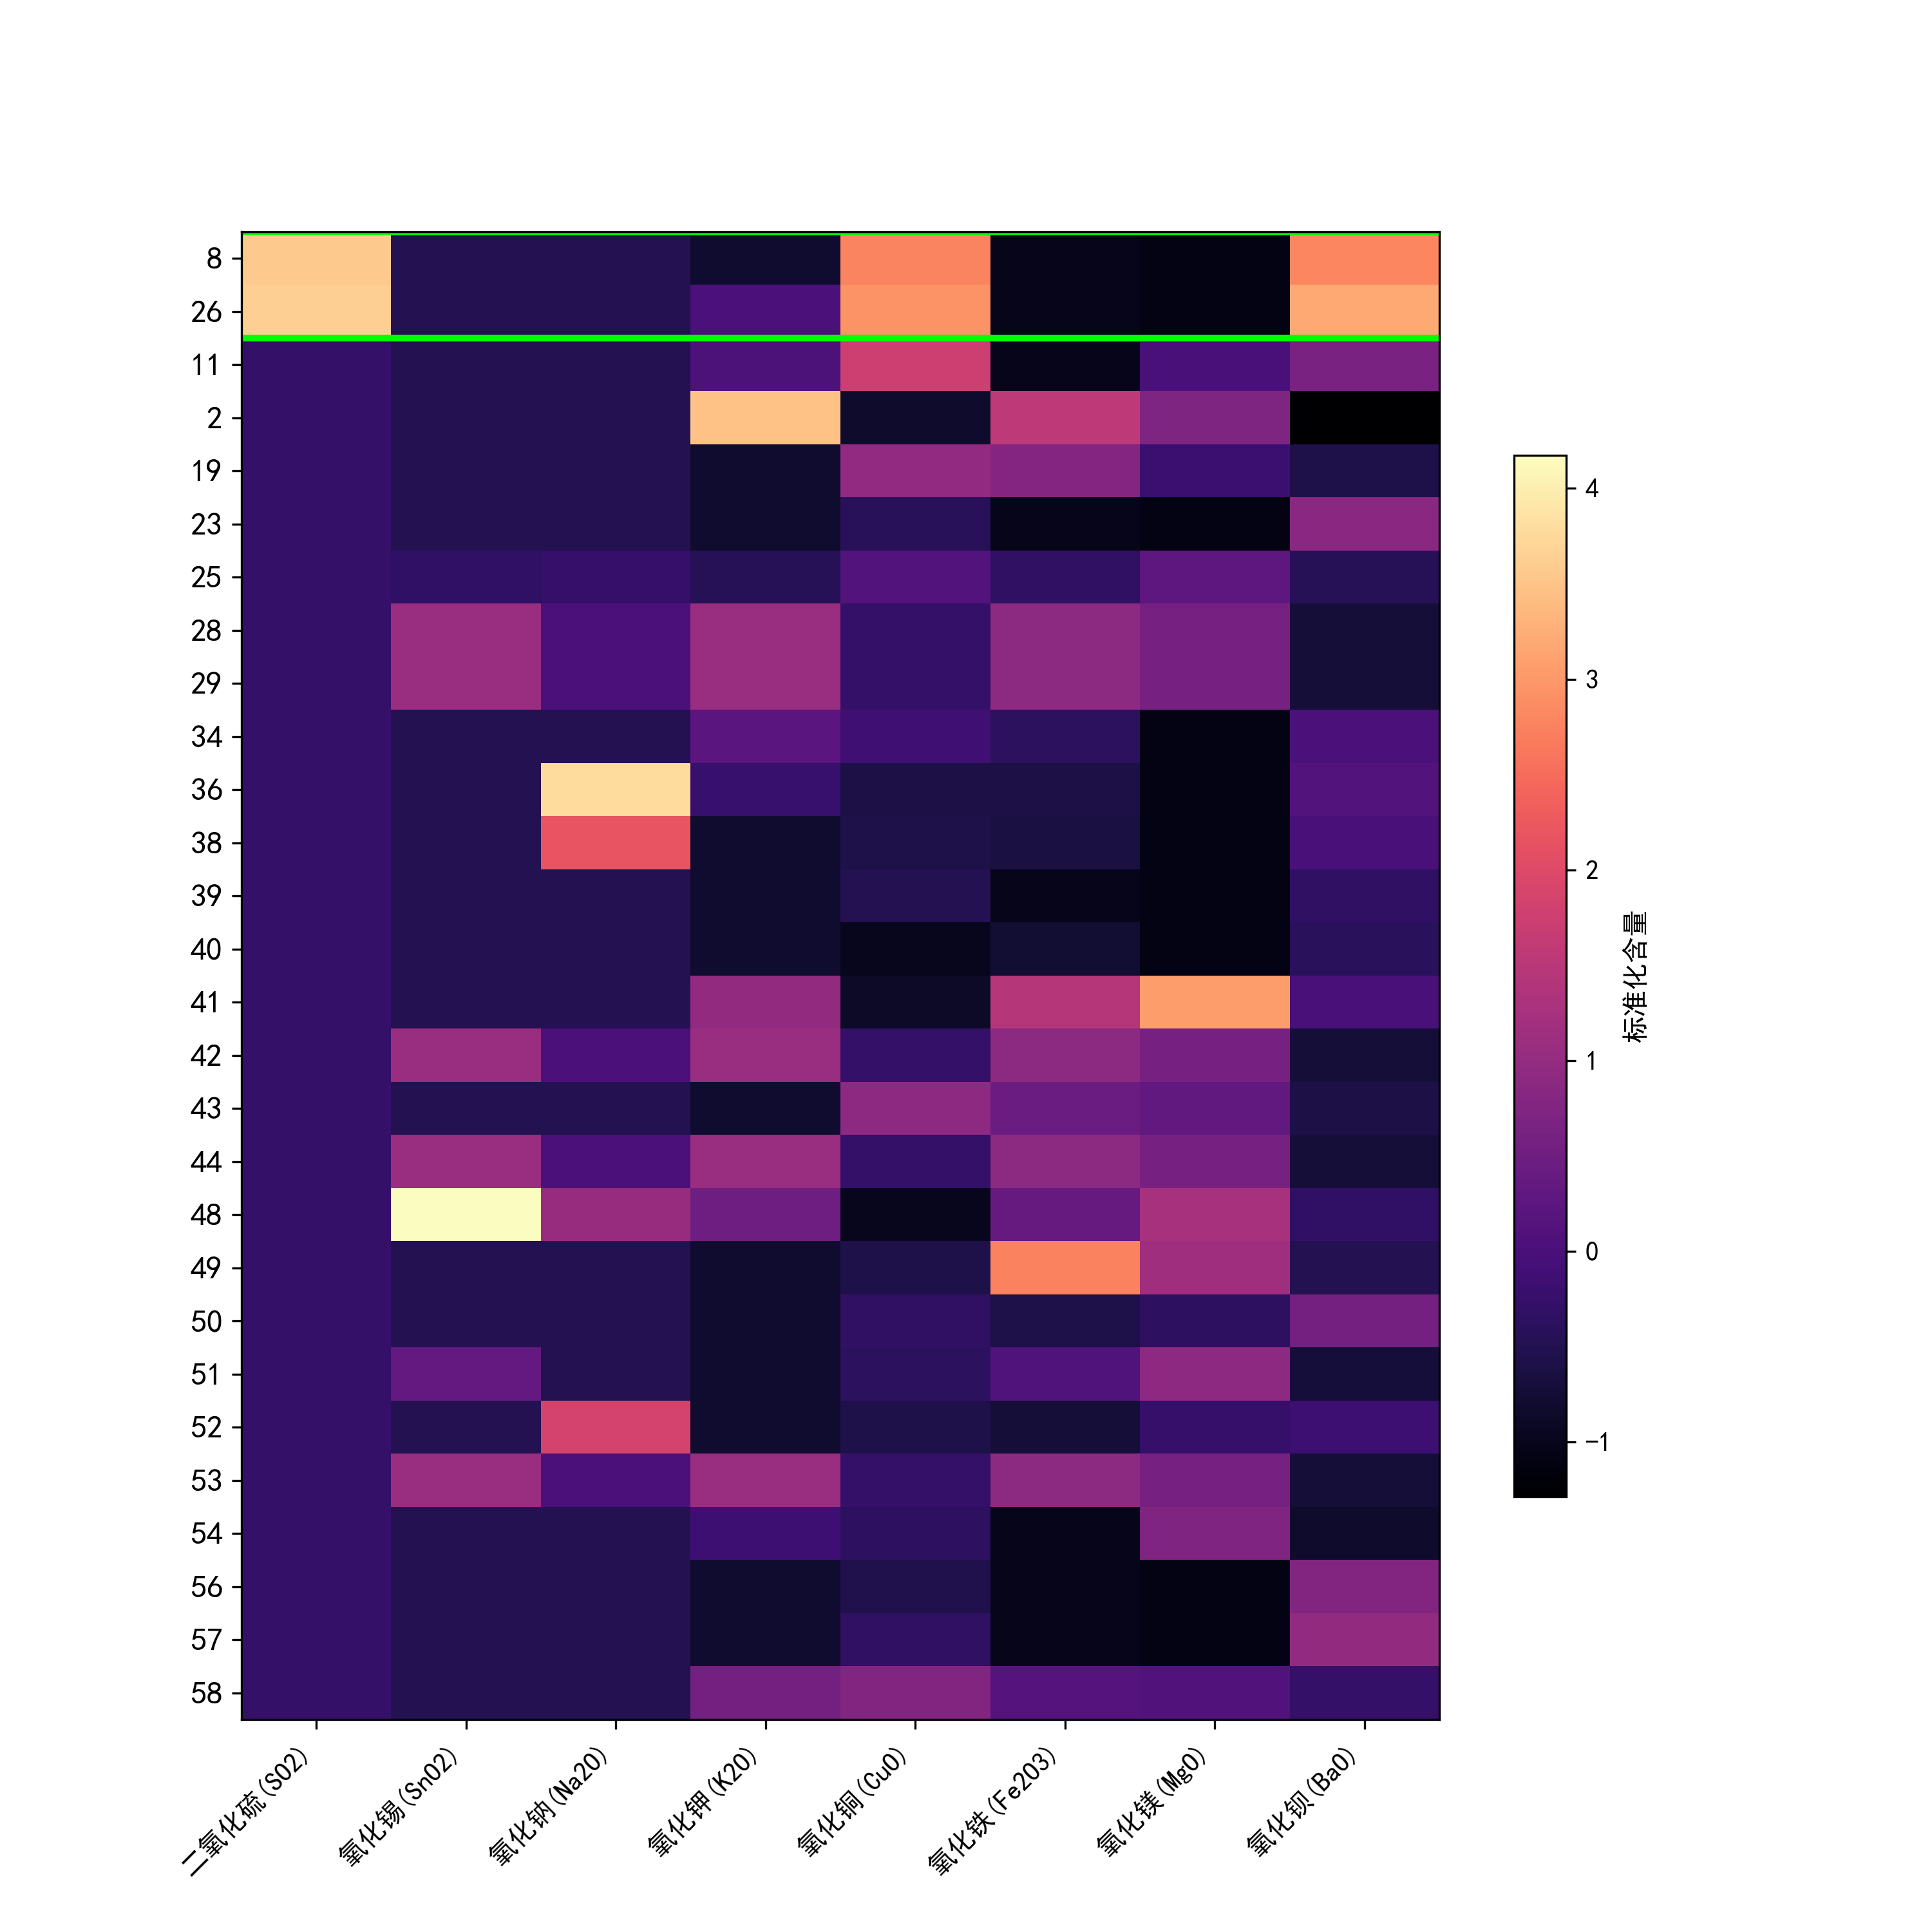
\includegraphics[width=\linewidth]{figs/4问题二/铅钡玻璃_亚类热力图_带编号.png}
        \caption{铅钡玻璃亚类化学特征热力图}
        \label{fig:heatmap_pb}
    \end{minipage}
\end{figure}

图\ref{fig:heatmap_pb}展示了铅钡玻璃两个亚类的化学差异。亚类一的样本在氧化铅$PbO$与氧化钡$BaO$两种助熔剂成分上呈现深色,表明其含量普遍较高,而作为玻璃基体的二氧化硅$SiO_2$含量则相对较低。与此相反,亚类零的样本在二氧化硅$SiO_2$上呈现深色,含量普遍较高,而氧化铅$PbO$与氧化钡$BaO$含量则较低。基于此,可将亚类一命名为高铅钡助熔剂型,亚类零命名为高硅基质型。

图\ref{fig:heatmap_k}则展现了高钾玻璃五个亚类更为细微的化学特征。亚类二的突出特征是其氧化钾$K_2O$含量极高,而其他成分含量较低。亚类一的氧化钙$CaO$含量相对突出。亚类零则表现为氧化铝$Al_2O_3$与氧化铁$Fe_2O_3$含量较高,这可能与其他亚类使用了不同的矿物原料有关。亚类三与亚类四的差异主要体现在磷与硫等微量元素上,反映了更为精细的原料或工艺差别。通过热力图分析,我们明确了每个亚类独特的化学成分特征。


\subsection{结果的敏感性分析}

为验证上述分类与划分结果的稳健性,我们进行了敏感性分析。首先,我们检验分类规律的可靠性。我们在十折交叉验证的每一次折叠中,重新训练线性支持向量机模型并提取其权重,以评估规律本身的稳定性。

\begin{figure}[H]
    \centering
    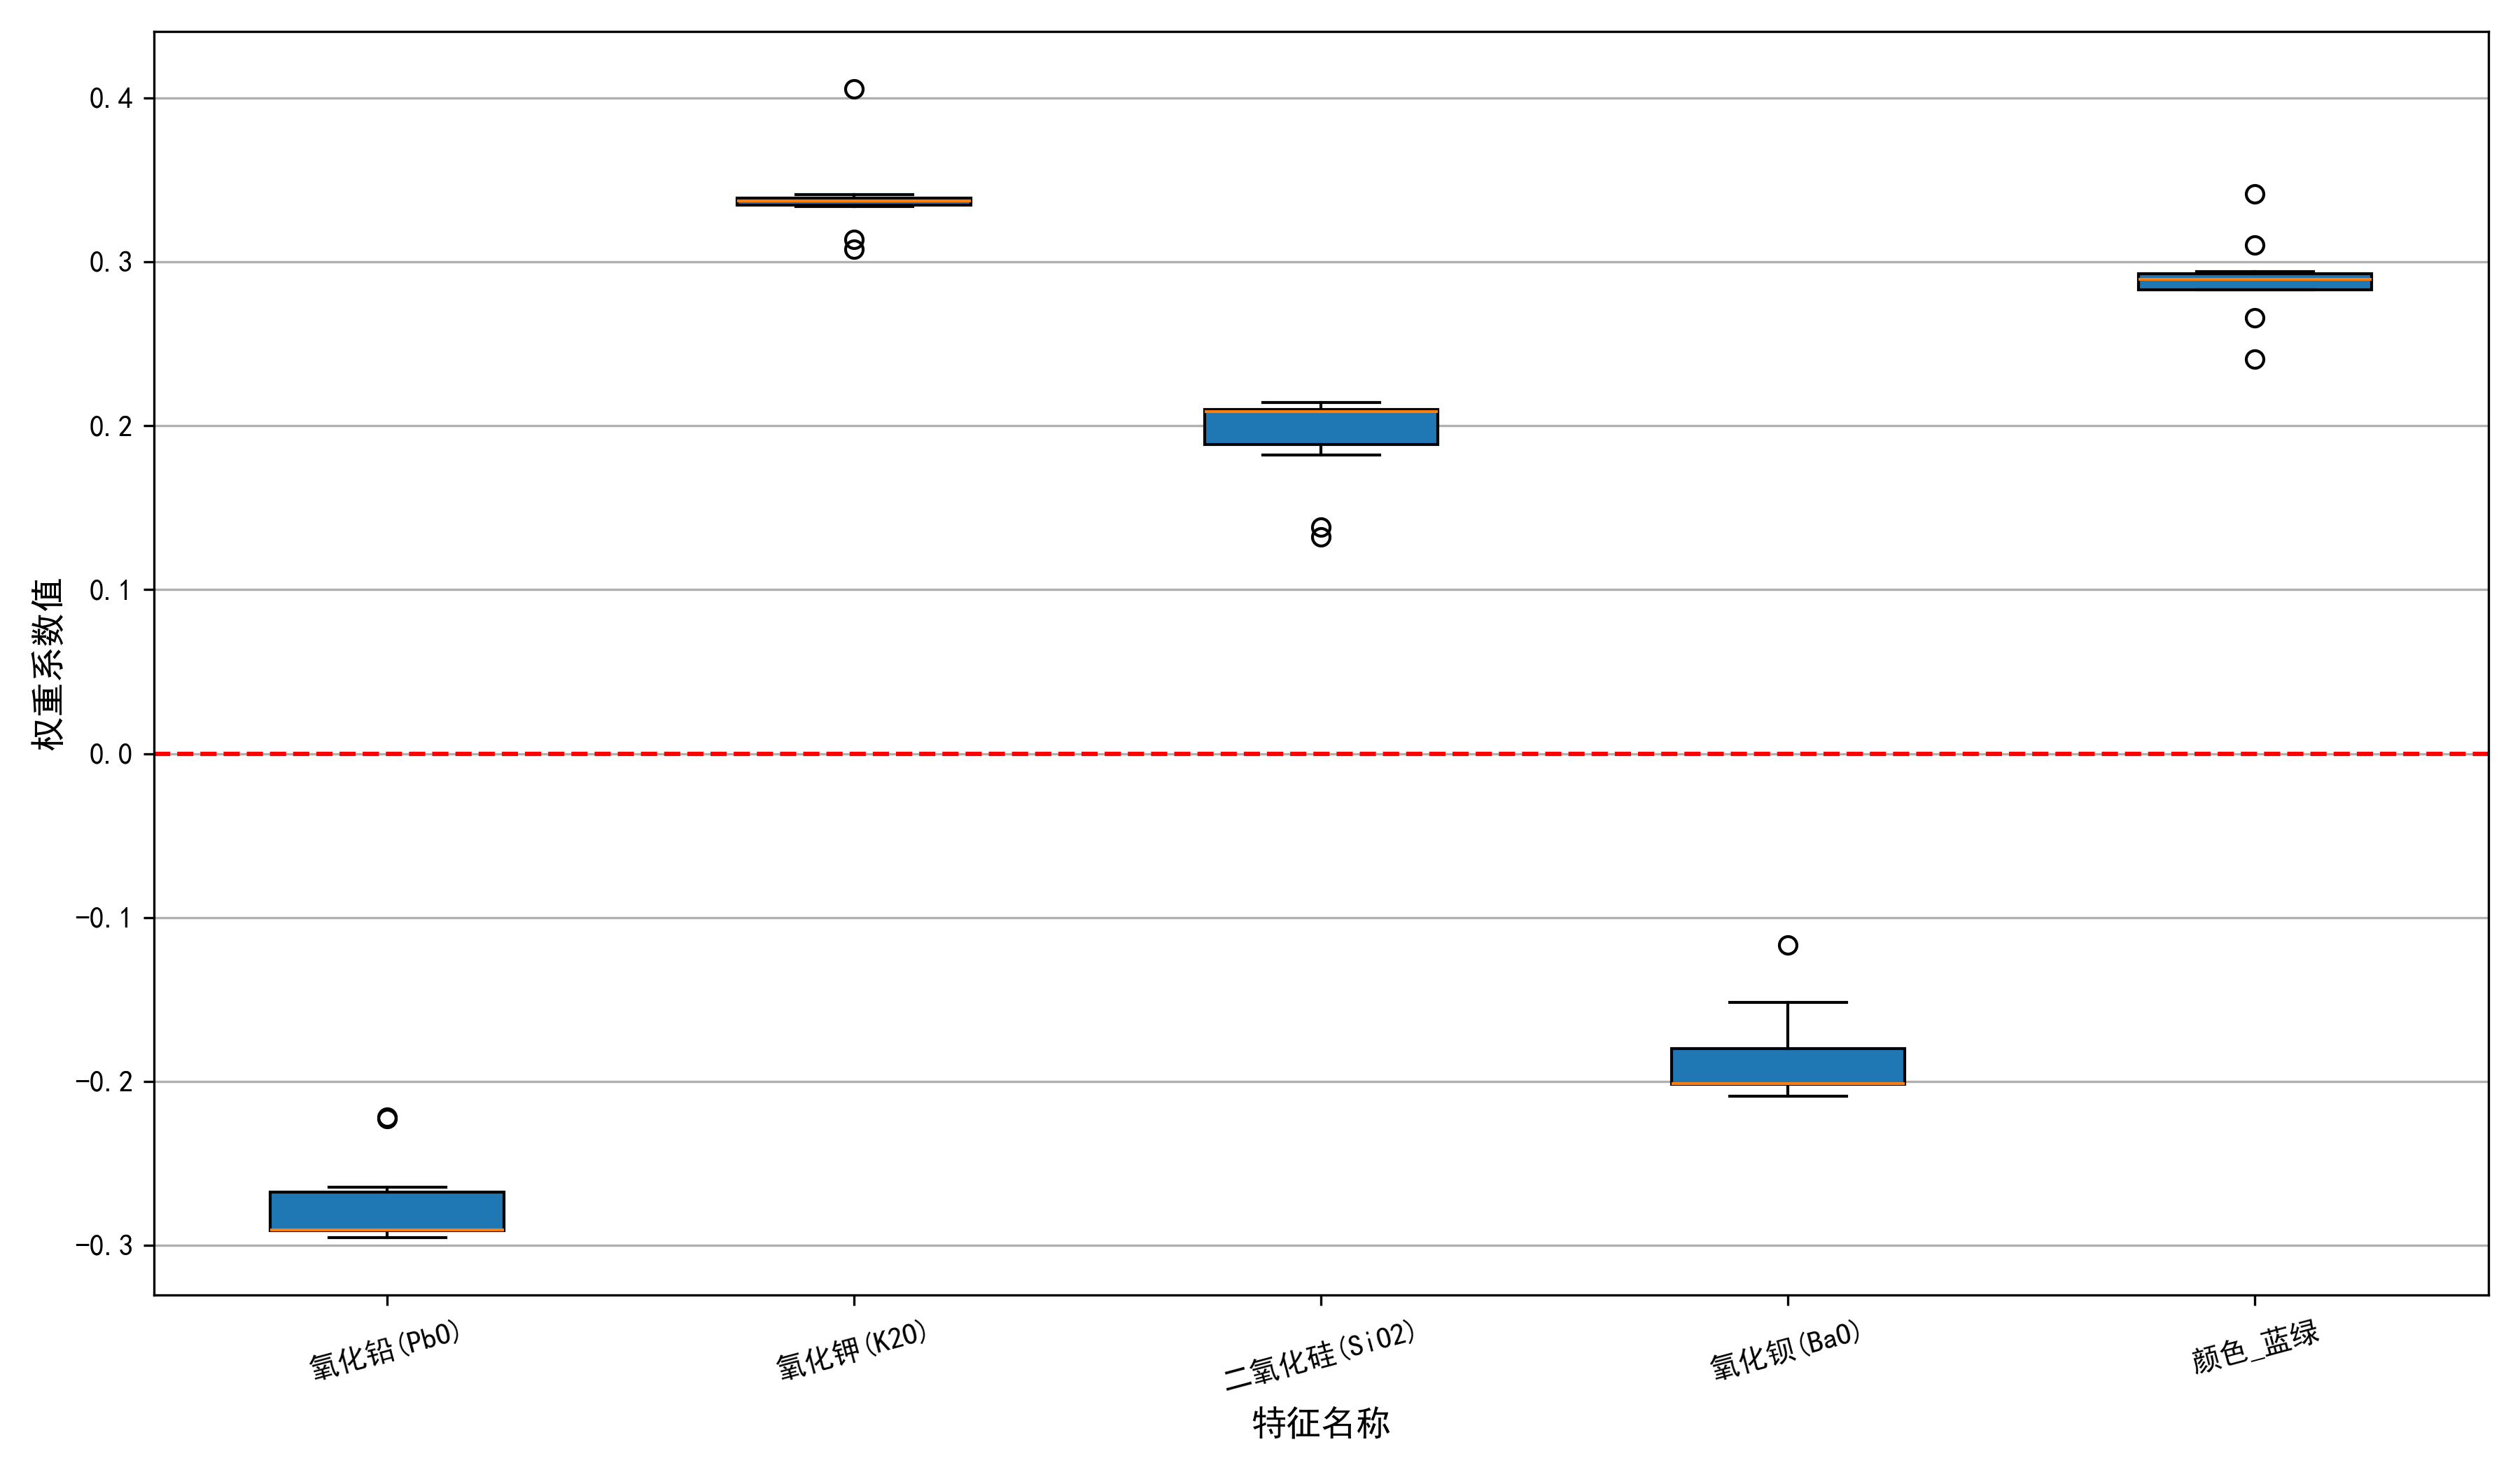
\includegraphics[width=\textwidth]{figs/4问题二/SVM权重稳定性分析.png}
    \caption{关键特征的SVM权重在十次交叉验证中的稳定性}
    \label{fig:svm_stability}
\end{figure}

图\ref{fig:svm_stability}通过箱线图展示了关键特征的权重在十次不同数据子集训练中的分布。图中显示,关键特征如$PbO$、$K_2O$的权重符号在十次实验中从未改变,且波动范围很小。这证明了我们提炼出的分类规律是高度稳健的。

其次,我们检验亚类划分结果的敏感性。为检验划分结果对化学成分测量误差的容忍度,我们采用了特征值扰动法。该方法通过向数据中注入不同水平的随机噪声,来模拟测量误差,并检验聚类结构的稳定性。我们对筛选出的特征数据乘以一个范围在$[1-p, 1+p]$内的随机扰动因子,其中$p$为扰动水平。在此扰动数据上重新聚类,并使用调整兰德指数$ARI$来衡量该次聚类结果与原始基准结果的一致性。

\begin{figure}[H]
    \centering
    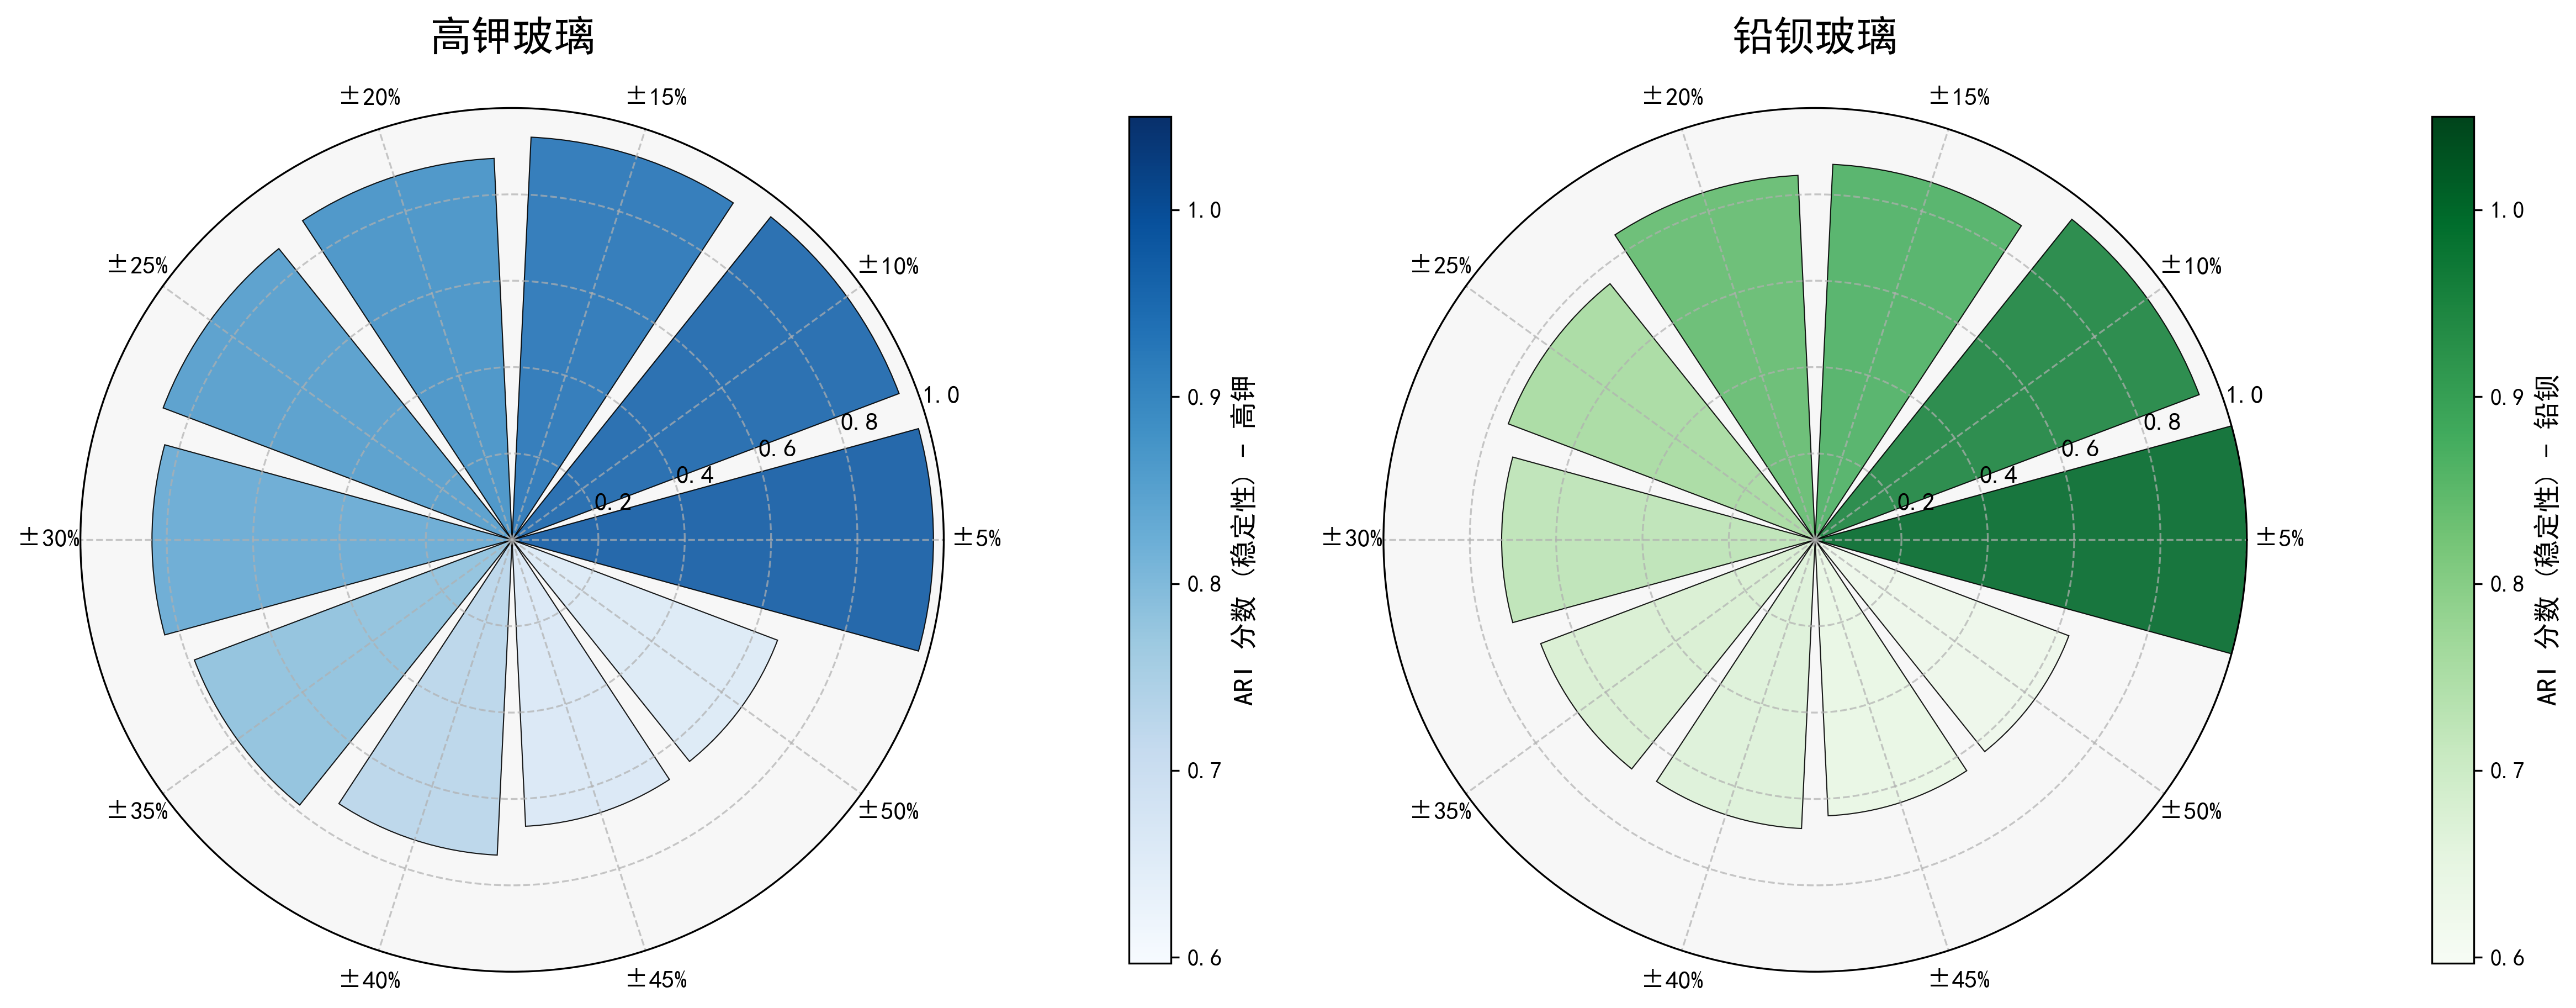
\includegraphics[width=\textwidth]{figs/4问题二/灵敏度分析_玫瑰图_ARI颜色映射.png}
    \caption{不同扰动水平下亚类划分结果的ARI分数}
    \label{fig:ari_sensitivity}
\end{figure}

图\ref{fig:ari_sensitivity}展示了在不同扰动水平下,高钾和铅钡玻璃亚类划分的平均ARI分数。对于高钾玻璃,即使在百分之十的扰动下,平均ARI分数依然高达0.9513。对于铅钡玻璃,在百分之十的扰动下,平均ARI分数为0.9596。在面临潜在的测量误差时,其核心划分依然能够保持高度一致。这证明了我们发现的亚类结构是真实且稳健的,而非随机产生的现象。



% \section{问题三:文物类别的鉴别与模型稳健性分析}

本章的核心任务是应用分类模型对未知类别玻璃文物的化学成分进行分析,确定其所属类型,并对分类结果的稳健性与可靠性进行系统性验证。为完成此任务,我们首先进行了一系列对比实验以选择最合适的模型架构,随后采用改进遗传算法对所选模型的超参数进行寻优,构建最终的分类器。最后,我们使用该模型进行预测,并通过双重灵敏度分析来检验结论的稳定性。其整体框架如图\ref{fig:model_framework}所示。

\begin{figure}[H]
    \centering
    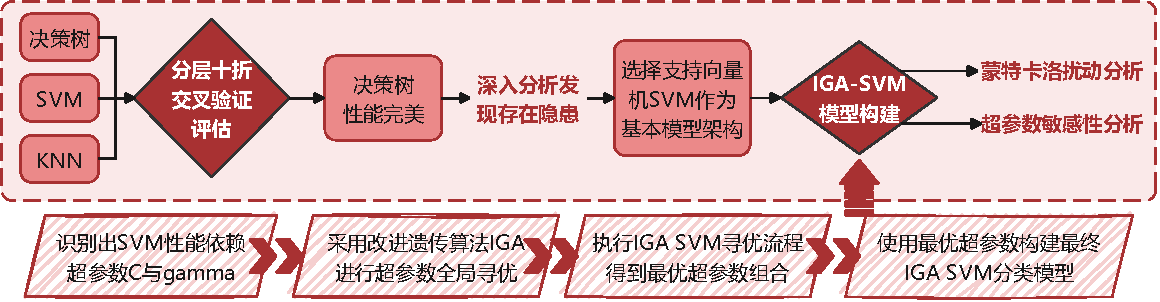
\includegraphics[width=\textwidth]{figs/5问题三/第三问框架.pdf}
    \caption{分类模型框架}
    \label{fig:model_framework}
\end{figure}

\subsection{分类模型的选择与论证}

为建立有效的分类规律,需要从多种候选模型中筛选出最适宜本数据特性的算法。我们选取决策树,K近邻算法以及支持向量机三种具有代表性的模型,在包含全部十四种化学成分及表面风化状况的完整特征集上进行初步性能评估。评估过程采用分层十折交叉验证方法,以保证每次训练与测试中样本类别的分布与原始数据保持一致。各模型的性能指标如表\ref{tab:model_performance}所示。

\begin{table}[H]
    \centering
    \caption{初步模型性能评估}
    \label{tab:model_performance}
    \begin{tabular}{lcc}
        \toprule
        \textbf{模型} & \textbf{准确率} & \textbf{F1分数} \\
        \midrule
        决策树 & 1.0000 & 1.0000 \\
        SVM & 0.9714 & 0.9576 \\
        KNN & 0.9857 & 0.9788 \\
        \bottomrule
    \end{tabular}
\end{table}

评估结果表明,决策树模型在所有性能指标上均达到了1.0的满分。为探究决策树模型取得此结果的原因,我们对其内部结构进行了分析。通过在完整的已分类数据集上训练单个决策树模型,我们发现其特征重要性得分几乎全部集中于氧化铅$PbO$这一项上。模型的可视化结构进一步确认了此发现,如图\ref{fig:decision_tree_structure}所示,该决策树仅在根节点依据氧化铅$PbO$含量是否大于一个特定阈值便完成了对所有样本的分类。

\begin{figure}[H]
    \centering
    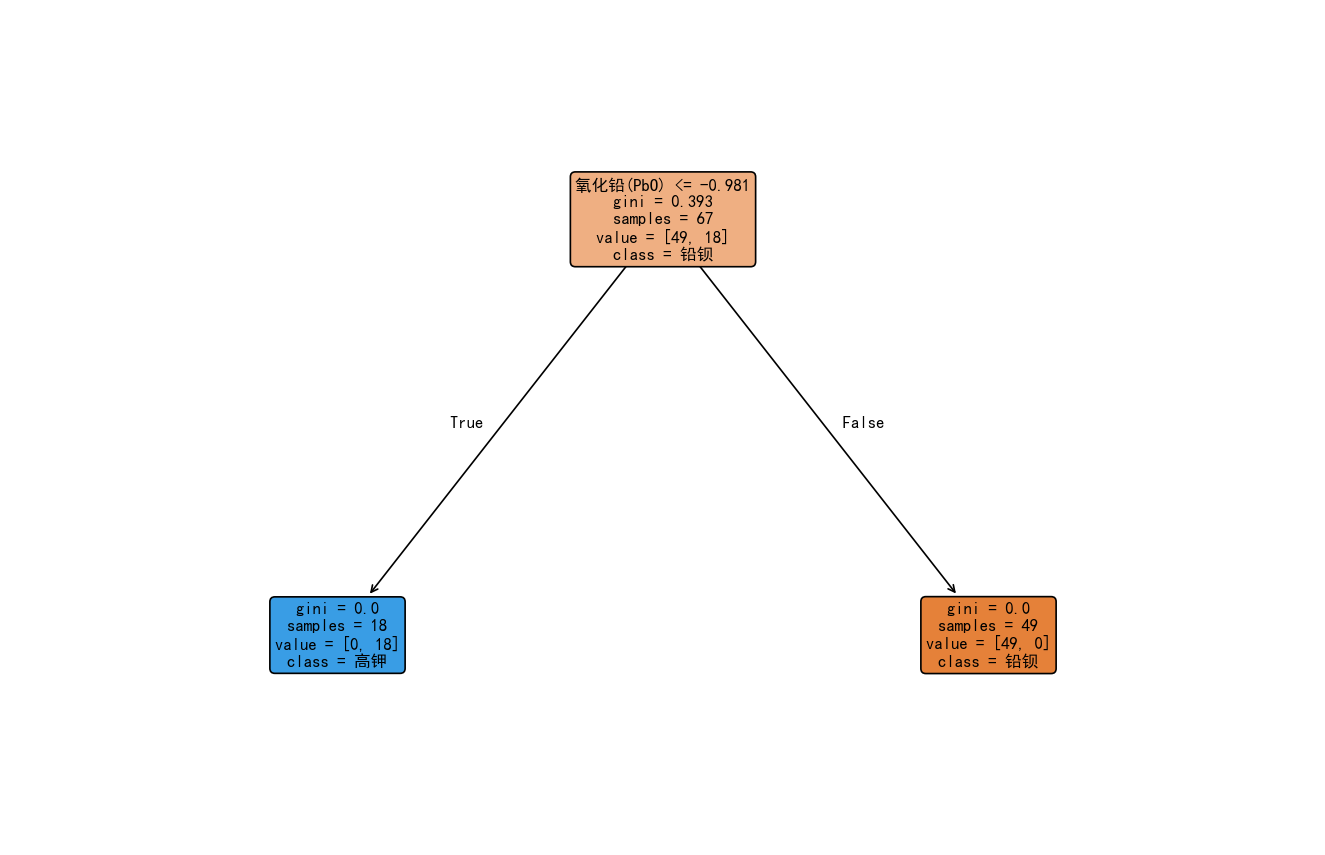
\includegraphics[width=0.8\textwidth]{figs/5问题三/初步决策树可视化图.png}
    \caption{初步决策树模型结构}
    \label{fig:decision_tree_structure}
\end{figure}

尽管决策树表现出很高的评分,但其过分依赖单一特征的决策模式存在稳健性隐患。一个仅凭氧化铅含量进行判断的模型,在面对不含氧化铅但仍属铅钡玻璃体系的未知样本时可能失效,其泛化能力不足。同时,由于该特征的存在,不同模型间的性能差异被掩盖,使得模型对比失去参考价值。基于这些考量,我们排除了将决策树作为最终模型的方案,转而寻求更能利用多维度信息且结构更为稳健的模型。在移除氧化铅特征后进行的补充实验中,支持向量机表现出优越的适应能力,因此我们选择支持向量机作为最终模型的基本架构。

\subsection{基于改进遗传算法的支持向量机模型构建}

支持向量机是一种在高维空间中寻找最优分类超平面的算法,其性能表现高度依赖于正则化系数$C$和核函数系数$\gamma$这两个超参数的设定。为充分发挥支持向量机的性能,我们采用改进遗传算法IGA来代替传统的网格搜索,对其超参数组合进行智能化全局寻优。

支持向量机的基本原理可表述为求解一个软间隔优化问题,其目标函数如下
\begin{equation}
    \min_{\boldsymbol{w}, b, \boldsymbol{\xi}} \frac{1}{2} ||\boldsymbol{w}||^2 + C \sum_{i=1}^{m} \xi_i
\end{equation}
式中$\boldsymbol{w}$与$b$定义了分类超平面,$\xi_i$是允许样本偏离正确边界的松弛变量,而$C$则用以平衡间隔最大化与分类误差。

改进遗传算法IGA是一种模拟生物进化过程的全局优化算法。它将超参数寻优过程转化为一个适者生存的演化过程。算法首先在预设的参数范围内随机生成一个包含多个个体即多组$C$与$\gamma$参数组合的初始种群。随后,算法以分层十折交叉验证的F1分数为适应度函数,对种群中每个个体的优劣进行评估。适应度越高的个体,在后续的遗传操作中被选中作为父代产生后代的概率越大。通过选择,交叉和变异这三种模拟自然繁殖过程的核心算子,算法不断迭代产生适应度更高的新一代种群。此外,精英保留策略确保了每一代的最优个体都能直接进入下一代,保证了寻优过程的收敛性。当达到预设的进化代数或种群适应度不再提升时,算法终止,并输出整个进化过程中适应度最高的个体所对应的超参数组合作为全局最优解。具体机制如\cref{alg:iga_svm}所示。

\begin{algorithm}[H]
    \caption{改进遗传算法IGA优化支持向量机超参数}
    \label{alg:iga_svm}
    \begin{algorithmic}[1]
        \Require
        \Statex 数据集 $D$
        \Statex 种群大小 $N$
        \Statex 最大进化代数 $G_{max}$
        \Statex 交叉概率 $p_c$
        \Statex 变异概率 $p_m$
        \Statex 超参数搜索空间 $S_C, S_{\gamma}$
        
        \Ensure
        \Statex 最优超参数组合 $(C_{best}, \gamma_{best})$

        \Function{IGA-SVM-Optimization}{$D, N, G_{max}, p_c, p_m, S_C, S_{\gamma}$}
            \State 初始化种群 $P_0$:随机生成 $N$ 个个体 $(C_i, \gamma_i)$,其中 $C_i \in S_C, \gamma_i \in S_{\gamma}$
            \State 定义适应度函数 $Fitness(C, \gamma) \leftarrow$ 使用 $(C, \gamma)$ 配置的SVM在数据集$D$上进行分层十折交叉验证的F1分数
            \For{$g = 1$ \textbf{to} $G_{max}$}
                \State 计算当前种群 $P_{g-1}$ 中每个个体的适应度
                \State $P_{new} \leftarrow \emptyset$ \Comment{初始化新一代种群}
                \State 寻找当前种群中的最优个体 $elite \leftarrow \arg\max_{i \in P_{g-1}} Fitness(i)$
                \State $P_{new} \leftarrow P_{new} \cup \{elite\}$ \Comment{精英保留策略}
                
                \For{$k = 1$ \textbf{to} $N-1$}
                    \State \Comment{通过遗传算子生成新个体}
                    \State $parent_1, parent_2 \leftarrow$ \Call{Select}{$P_{g-1}$} \Comment{根据适应度选择父代}
                    \If{$\text{random}(0,1) < p_c$}
                        \State $child \leftarrow$ \Call{Crossover}{$parent_1, parent_2$} \Comment{交叉操作}
                    \Else
                        \State $child \leftarrow parent_1$ \Comment{直接复制}
                    \EndIf
                    
                    \If{$\text{random}(0,1) < p_m$}
                        \State $child \leftarrow$ \Call{Mutate}{$child$} \Comment{变异操作}
                    \EndIf
                    
                    \State $P_{new} \leftarrow P_{new} \cup \{child\}$
                \EndFor
                \State $P_g \leftarrow P_{new}$ \Comment{更新种群}
            \EndFor
            
            \State $(C_{best}, \gamma_{best}) \leftarrow \arg\max_{i \in P_{G_{max}}} Fitness(i)$ \Comment{找出最终的最优个体}
            \State \Return $(C_{best}, \gamma_{best})$
        \EndFunction
    \end{algorithmic}
\end{algorithm}

在具体实现中,我们配置了一个包含15个个体,进化30代的遗传算法。其寻优过程如图\ref{fig:iga_process}所示,该三维瀑布图展示了在迭代过程中,种群的最高适应度,平均适应度与最低适应度的变化情况。图中可见,种群的整体适应度随着进化代数的增加而快速上升并趋于稳定,表明该算法能够高效地在参数空间中搜索到最优解区域。

\begin{figure}[H]
    \centering
    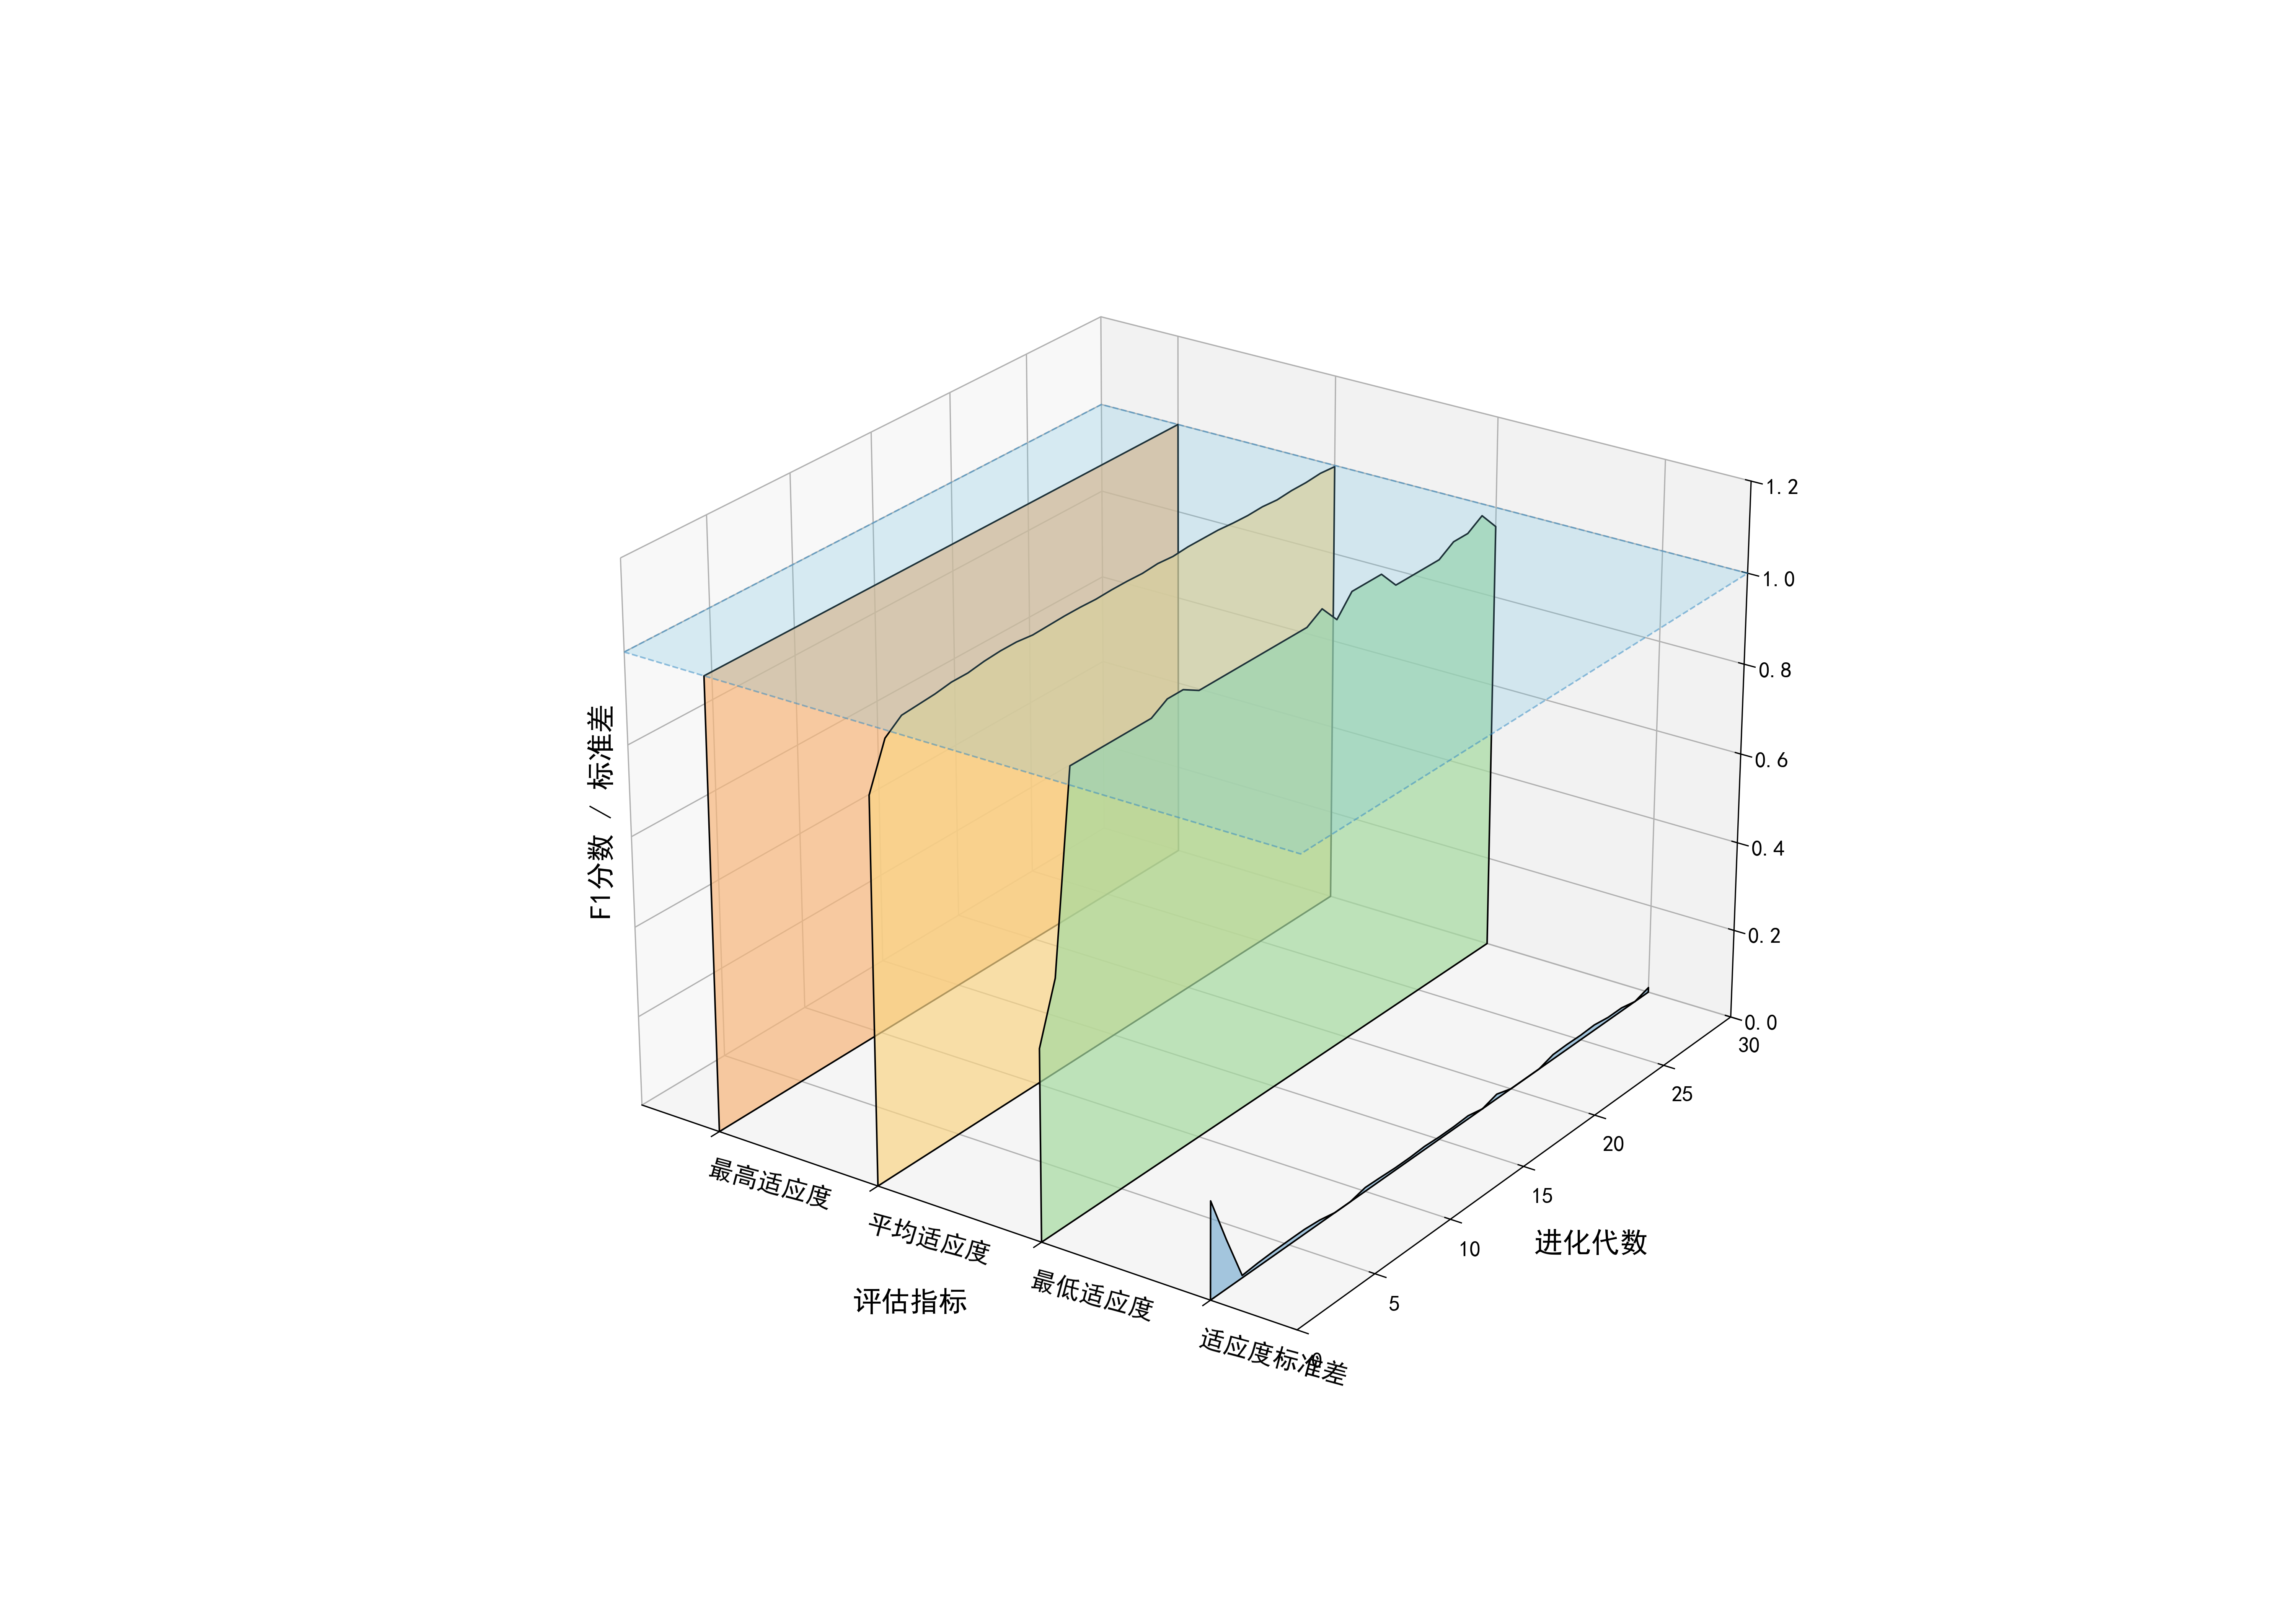
\includegraphics[width=\textwidth]{figs/5问题三/IGA_SVM寻优过程3D瀑布图_最终版.png}
    \caption{改进遗传算法寻优过程}
    \label{fig:iga_process}
\end{figure}

\subsection{最终鉴别结果与双重可靠性验证}

利用前述流程寻得的最优超参数构建最终的IGA-SVM分类模型后,我们将其应用于8个未知类别样本的化学成分数据,完成了最终的类别鉴别。其具体的预测结果如表\ref{tab:prediction_results}所示。

\begin{table}[H]
    \centering
    \caption{未知样本最终预测结果}
    \label{tab:prediction_results}
    \begin{tabular}{|c|c|c|c|c|c|c|c|c|}
        \hline
        \textbf{样本标识} & 0 & 1 & 2 & 3 & 4 & 5 & 6 & 7 \\
        \hline
        \textbf{预测类别} & 高钾 & 铅钡 & 铅钡 & 铅钡 & 铅钡 & 高钾 & 高钾 & 铅钡 \\
        \hline
    \end{tabular}
\end{table}

以确保鉴别结果的可靠性,我们从数据与模型两个维度设计了双重灵敏度分析方案。第一重分析是蒙特卡洛扰动分析,用以检验预测结论对于数据测量误差的稳健性。我们进行了1000次模拟实验,在每次实验中,对样本的部分化学成分数据加入0至5个百分点的随机噪声,然后使用模型重新进行预测。我们通过计算每个样本预测结果在1000次扰动中发生改变的频率,来量化其预测不稳定性。实验结果显示,所有样本的预测不稳定性得分均为0,这表明鉴别结论对于一定范围内的测量误差具有高度的稳定性。

第二重分析是支持向量机超参数敏感性分析,用以检验预测结论对于模型参数选择的稳健性。我们围绕寻得的最优$C$与$\gamma$值构建了一个5乘5的参数网格。对于网格中的每一对参数组合,我们都重新训练支持向量机模型并对未知样本进行预测,然后记录其预测结果与原始最优模型结果不一致的样本数量。分析结果通过热力图进行可视化,如图\ref{fig:svm_sensitivity}所示。

\begin{figure}[H]
    \centering
    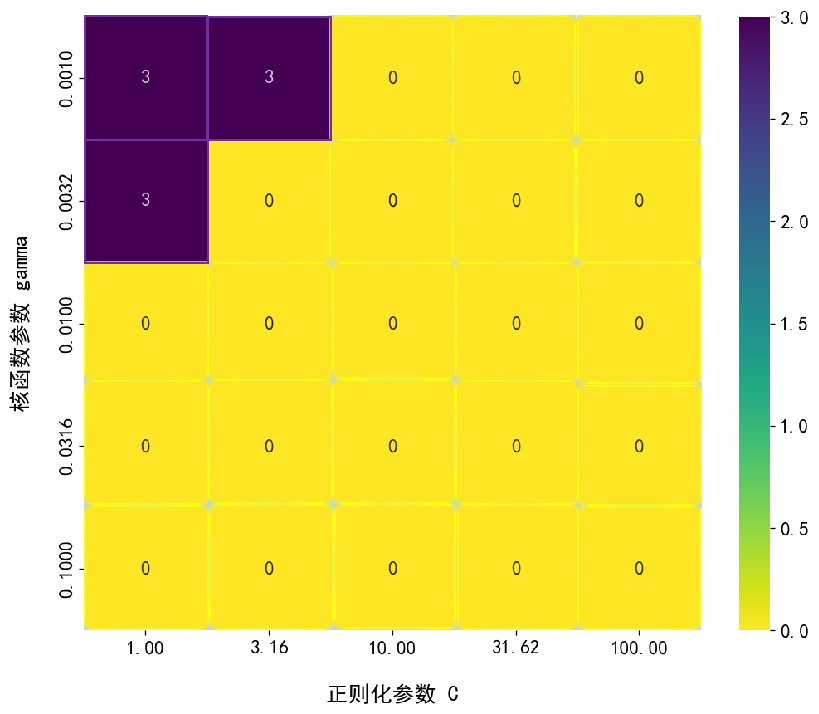
\includegraphics[width=0.7\textwidth]{figs/5问题三/SVM超参数敏感性分析热图.png}
    \caption{支持向量机超参数敏感性分析}
    \label{fig:svm_sensitivity}
\end{figure}

图\ref{fig:svm_sensitivity}中,每个方格的颜色代表在该参数对下预测结果发生改变的样本数量,颜色越深表示变化越大。图中可见,在以最优参数点为中心的广大区域内,颜色均为最浅色,对应数值为0,这意味着预测结果没有发生任何改变。这一广阔的稳定区域证明,最终的鉴别结论对模型超参数的选择不敏感,并非是在某个特定参数点上偶然获得的结果,从而进一步确认了结论的可靠性。

% \section{灵敏度分析}

前述模型是基于一系列经济与生产参数构建的,这些参数在现实世界中天然存在波动性。为了评估模型所得方案的可靠性与稳定性,本章将进行系统的灵敏度分析。此分析旨在探究最优种植方案对关键参数变化的响应程度,检验方案在不同市场环境下的表现,并验证模型结构中关键假设的合理性与价值。

\subsection{问题一确定性模型的灵敏度分析}

问题一的混合整数线性规划模型建立在所有输入参数均为确定值的基础上。然而,市场价格、生产成本与作物产量等均是动态变化的。因此,本节的分析旨在检验确定性最优种植方案对这些核心经济参数波动的敏感程度,识别对总利润影响最显著的因素,并评估方案在宏观市场变化情景下的稳健性。

分析的第一步是单因素扰动分析,用以探究单一参数变化对整体结果的独立影响。首先,基于基准模型求解得到的最优种植方案,识别出对七年总利润贡献度最高的若干种核心作物。这些作物的销售价格($P_{jy}$)、种植成本($C_{jy}$)与单位面积产量($\text{yield}_{jy}$)被选为关键扰动参数。在分析过程中,每次仅选择一个参数,在其基准值的基础上进行特定范围的扰动,例如$\pm 5\%$至$\pm 20\%$。在保持其他参数不变的条件下,重新求解优化模型,记录总利润的变化。为量化模型对参数的敏感程度,定义灵敏度系数$S$如下:

\begin{equation}
    S = \frac{\Delta \text{Profit} / \text{Profit}_{\text{base}}}{\Delta \text{Parameter} / \text{Parameter}_{\text{base}}}
\end{equation}

其中,$\Delta \text{Profit}$与$\Delta \text{Parameter}$分别代表总利润与参数值相对于基准值的变化量。该过程对所有已识别的关键参数重复进行。

% \begin{figure}[H]
%     \centering
%     \includegraphics[width=0.8\textwidth]{figs/灵敏度/单因素分析图.png}
%     \caption{关键参数的单因素灵敏度分析结果}
%     \label{fig:sen_p1_single}
% \end{figure}

图\ref{fig:sen_p1_single}展示了各关键参数的灵敏度系数。系数的绝对值$|S|$越大,表明总利润对该参数的波动越敏感。从图中结果可知,部分高价值蔬菜的销售价格与单位面积产量是影响最终收益的关键因素。这些被识别出的高敏感性参数构成了种植决策中的核心风险源,在实际生产管理中需要得到重点关注与监控。

为进一步模拟真实市场环境的复杂性,我们进行了多因素情景分析。该分析旨在评估基准最优方案在面对系统性冲击时的整体表现。为此,构建了三个具有代表性的宏观市场情景:情景A(通货膨胀),假设所有作物的种植成本普遍上涨15\%;情景B(市场利好),假设蔬菜类作物的销售价格普遍上涨20\%,粮食类价格稳定;情景C(供给冲击),假设因气候不利,所有露天作物的单位面积产量下降10\%。将问题一求解出的固定最优种植方案$a_{ijky}^*$分别置于这三种情景下,重新计算其七年总利润,而不进行重新优化。

% \begin{figure}[H]
%     \centering
%     \includegraphics[width=0.8\textwidth]{figs/灵敏度/情景分析图.png}
%     \caption{最优方案在不同市场情景下的利润表现}
%     \label{fig:sen_p1_scenario}
% \end{figure}

图\ref{fig:sen_p1_scenario}对比了基准利润与各情景下的利润。结果显示,在成本上涨(情景A)和产量下降(情景C)的不利条件下,方案的总利润出现了不同程度的下滑。利润下降的幅度是衡量该方案稳健性的直接指标。若下降幅度相对较小,则表明该方案能够较好地抵御相应类型的市场风险。反之,较大的利润损失则说明该方案高度依赖于初始的市场假设,在面对特定类型的风险时表现脆弱,提示决策者需要为这类市场风险准备应对预案。

\subsection{问题二鲁棒优化模型的灵敏度分析}

问题二鲁棒优化模型的核心在于不确定集$U$的定义,其目标是在该集合内的所有可能场景中寻求最坏情况下的最优解。因此,本节的灵敏度分析旨在检验最优保底利润及对应的种植方案对不确定集定义的依赖程度,并量化风险规避水平与保证收益之间的权衡关系。

分析的核心是扰动不确定集的大小。模型中的不确定参数(如价格、产量)的波动范围由一个波动系数$\delta$决定。我们将$\delta$作为关键扰动参数,通过设定一系列递增的$\delta$值(例如从5\%至25\%),构建不同大小的不确定集$U$,并对每个$U$重新求解相应的鲁棒优化模型。此过程记录了在每个$\delta$值下,模型所能实现的最优年度平均保底利润$\Gamma^*$。

% \begin{figure}[H]
%     \centering
%     \includegraphics[width=0.8\textwidth]{figs/灵敏度/鲁棒分析图.png}
%     \caption{保底利润随不确定集波动范围 ($\delta$) 的变化关系}
%     \label{fig:sen_p2_robust}
% \end{figure}

图\ref{fig:sen_p2_robust}绘制了最优保底利润$\Gamma^*$与波动系数$\delta$之间的关系。图中清晰地呈现出一条向下倾斜的曲线,这直观地揭示了鲁棒性的“代价”。为了抵御更大范围的市场风险(即更大的$\delta$值),决策者必须接受一个相对较低的保底利润水平。这条有效前沿曲线为决策者在风险与回报之间进行权衡提供了定量的决策依据。

鲁棒模型提供的是一个抗风险方案,但其在随机未来中的期望表现需要通过后验模拟检验。为此,我们选取了不同鲁棒水平下的最优种植方案(例如$\delta=10\%$和$\delta=20\%$得到的方案$a_{10\%}^*$和$a_{20\%}^*$),并以问题一的确定性最优方案$a_{\text{det}}^*$作为基准进行对比。通过蒙特卡洛方法生成大量随机市场情景,将这三个固定的种植方案分别代入每一个随机情景中计算利润,从而得到每个方案的利润概率分布。我们基于期望利润、利润标准差以及条件风险价值(CVaR)等统计指标对方案进行量化评估。

% \begin{figure}[H]
%     \centering
%     \includegraphics[width=0.8\textwidth]{figs/灵敏度/后验模拟图.png}
%     \caption{确定性方案与鲁棒方案在后验模拟中的利润分布与风险指标对比}
%     \label{fig:sen_p2_posterior}
% \end{figure}

图\ref{fig:sen_p2_posterior}展示了后验模拟的结果。结果表明,鲁棒方案的期望利润可能略低于确定性方案,但其利润分布更为集中,表现为更低的标准差和显著改善的CVaR指标。这定量地证明了鲁棒模型在风险管理方面的价值:通过牺牲少量在理想情况下的最优期望收益,换取了在不利情况下风险的显著降低,提升了方案在不确定环境下的整体表现。

\subsection{问题三动态反馈模型的灵敏度分析}

问题三模型引入了描述市场反馈的非线性关系,其核心参数为成本敏感度系数$\alpha_j$与价格敏感度系数$\beta_j$。这些系数是基于对市场行为的假设设定的,其取值的准确性对模型结果有直接影响。本节分析旨在检验模型结果对这些关键行为参数的敏感性,并从根本上验证引入市场反馈这一复杂结构的必要性。

首先,我们对关键的敏感度系数进行扰动分析。这些系数由更底层的假设(例如,某作物产量超出基准10\%时,其价格下降$k_j$\%)推导而来。我们针对利润贡献最高的几种作物,对其价格下降率$k_j$和成本上涨率$m_j$的基准设定进行不同程度的扰动。每次扰动后,重新计算对应的$\alpha_j$和$\beta_j$,并完整运行整个“启发式算法+蒙特卡洛”求解流程,得到一个新的最优期望总利润$E[Z]^*$。

% \begin{figure}[H]
%     \centering
%     \includegraphics[width=0.8\textwidth]{figs/灵敏度/敏感系数扰动图.png}
%     \caption{最优期望利润对关键作物市场敏感度系数的响应}
%     \label{fig:sen_p3_coeffs}
% \end{figure}

图\ref{fig:sen_p3_coeffs}展示了最优期望利润$E[Z]^*$随关键敏感度参数变化的响应情况。若$E[Z]^*$随参数变化表现出剧烈波动,则说明模型结果对市场弹性的假设高度敏感。这一结果提示,为了获得更可靠的决策支持,有必要投入更多资源以获取更准确的市场反应数据,从而降低模型的不确定性。

为了验证模型中引入市场反馈效应的必要性,我们设计了对照情景分析。我们构建了一个不包含市场反馈的简化版模型作为对照组。具体而言,在该模型中,强制将所有作物的成本敏感度系数$\alpha_j$和价格敏感度系数$\beta_j$均设为0,并移除所有与作物替代或互补相关的销量修正规则。该简化模型在本质上退化为一个仅考虑参数随机波动但无市场反馈的随机优化模型。我们使用相同的算法求解该简化模型,得到一个“无关联”情景下的最优期望利润$E[Z]_{\text{no-corr}}^*$及其对应的种植方案$a_{\text{no-corr}}^*$。

% \begin{figure}[H]
%     \centering
%     \includegraphics[width=0.8\textwidth]{figs/灵敏度/对照分析图.png}
%     \caption{完整模型与“无关联”对照模型的最优期望利润对比}
%     \label{fig:sen_p3_control}
% \end{figure}

图\ref{fig:sen_p3_control}对比了完整模型与“无关联”对照模型求解得到的最优期望利润。结果显示,完整模型得到的最优期望利润$E[Z]^*$显著高于对照模型的$E[Z]_{\text{no-corr}}^*$。这一差异有力地证明了在模型中考虑市场关联效应的价值。通过将市场反馈纳入决策过程,模型能够指导种植策略主动规避因过度生产导致的“增产不增收”陷阱,从而找到在真实市场环境下表现更优的方案,创造了额外的经济价值。









\newpage

% 参考文献
\bibliographystyle{plain}
\bibliography{reference}
\newpage

\end{document}